\documentclass[a4paper,11pt]{report}

\usepackage[utf8]{inputenc}

\usepackage[a4paper, asymmetric, right=2.5cm, left=3.0cm, top=2.5cm, bottom=2.0cm]{geometry}

\usepackage[german, english]{babel}
\usepackage[left]{eurosym}
\usepackage{tabularx}
\newcolumntype{v}[1]{%
  >{\raggedright\hspace{Opt}}p{#1}%
}  
\usepackage{slashbox}

\usepackage{tikz}
\usetikzlibrary{arrows}
\usetikzlibrary{shapes}
\usetikzlibrary{plotmarks}
\usetikzlibrary{snakes}
\usetikzlibrary{backgrounds,positioning}
\usepackage{amsmath}
\usepackage{amsfonts}
\usepackage{amssymb}
\usepackage{makeidx}
%\usepackage{multind}
\usepackage{tocbibind}
\usepackage{nicefrac}
\usepackage{thumbpdf}


\usepackage[draft=false, plainpages=false,
						colorlinks=true, linkcolor=blue, citecolor=blue, urlcolor=red,	
						bookmarks, bookmarksopen, bookmarksopenlevel=1, bookmarksnumbered=true,breaklinks=true,
						pdftitle={The GrGen User Manual},
						pdfauthor={Jakob Blomer, Rubino Geiss},
						pdfkeywords={
						graph, graph transformation, graph rewriting, tool, spo, manual, grgen, graph rewrite generator,
						University of Karlsruhe, IPD Goos},
						pdfpagelabels
						]{hyperref}

\usepackage[all]{xy}
\usepackage{xcolor}
\definecolor{light}{gray}{0.8}
\definecolor{tuerkis}{cmyk}{0.5,0.15,0,0.3}
\usepackage{wrapfig}
\usepackage{graphicx}
\usepackage{calc}

%\usepackage{listings}
%\lstset{language=C, numbers=left, numberstyle=\tiny, stepnumber=5}

\providecommand{\O}[1]{\ensuremath{\mathcal{O}\left( #1 \right)}}

\providecommand{\N}{\ensuremath{\mathbb{N}}}
\providecommand{\Z}{\ensuremath{\mathbb{Z}}}
\renewcommand{\P}{\ensuremath{\mathbb{P}}}
\providecommand{\F}{\ensuremath{\mathbb{F}}}
\providecommand{\Q}{\ensuremath{\mathbb{Q}}}
\providecommand{\R}{\ensuremath{\mathbb{R}}}
\providecommand{\C}{\ensuremath{\mathbb{C}}}

\providecommand{\abs}[1]{\left\lvert #1 \right\rvert}
\providecommand{\norm}[1]{\left\lVert #1 \right\rVert}
\providecommand{\floor}[1]{\left\lfloor #1 \right\rfloor}
\providecommand{\svert}{\; \vert \;}

\DeclareMathOperator{\Abb}{Abb}   % Abbildungsmenge
\DeclareMathOperator{\Sym}{Sym}   % Bijektionenmenge
\DeclareMathOperator{\Hom}{Hom}   % Homomorphismenmenge
\DeclareMathOperator{\End}{End}   % Endomorphismenmenge
\DeclareMathOperator{\Aut}{Aut}   % Automorphismenmenge
\DeclareMathOperator{\deF}{def} 
\DeclareMathOperator{\ran}{ran} 
\DeclareMathOperator{\lhs}{lhs} 
\DeclareMathOperator{\rhs}{rhs} 

\providecommand{\id}{\ensuremath{\textsf{id}}}  % identische Abbildung
\DeclareMathOperator{\Kern}{Kern}     % Kern
\DeclareMathOperator{\Bild}{Bild}     % Bild

\providecommand{\Bin}[2]{\ensuremath{\operatorname{Bin} \left( #1 , #2 \right)}}
\providecommand{\Hyp}[2]{\ensuremath{\operatorname{Hyp} \left( #1 , #2 \right)}}

\providecommand{\PeroW}[2]{\ensuremath{\text{Per}^{#1}_{#2}\text{(oW)}}}
\providecommand{\PermW}[2]{\ensuremath{\text{Per}^{#1}_{#2}\text{(mW)}}}
\providecommand{\KomoW}[2]{\ensuremath{\text{Kom}^{#1}_{#2}\text{(oW)}}}
\providecommand{\KommW}[2]{\ensuremath{\text{Kom}^{#1}_{#2}\text{(mW)}}}

\makeatletter
\def\Relbar{\mathrel{\smash=}}
\def\Leftarrowfill@{\arrowfill@\Leftarrow\Relbar\Relbar}
\def\Rightarrowfill@{\arrowfill@\Relbar\Relbar\Rightarrow}
\newcommand{\xRightarrow}[2][]{\ext@arrow 0359\Rightarrowfill@{#1}{#2}}
\newcommand{\xLeftarrow}[2][]{\ext@arrow 3095\Leftarrowfill@{#1}{#2}}
\makeatother 

\usepackage{rail}
\railalias{lbrace}{\{}
\railalias{rbrace}{\}}
\railalias{underscore}{\_}
\railalias{dollar}{\$}
\railalias{percent}{\%}
\railalias{ampersand}{<>}
\railalias{backslash}{\char"5C}
\railalias{tilde}{$\sim$}
\railalias{ampersand}{\&}
\railalias{doubleampersand}{\&\&}
\railalias{etc}{$\cdots$}
\railalias{xorhat}{$\wedge$}

\railalias{analyzegraph}{analyze\_graph}
\railalias{gensearchplan}{gen\_searchplan}
\railalias{setmaxmatches}{set\_max\_matches}

\railterm{lbrace,rbrace,dollar,percent,ampersand,backslash,underscore,tilde,ampersand,analyzegraph, gensearchplan,setmaxmatches,doubleampersand,xorhat}

\usepackage[final]{listings}

\usepackage{soul}
\usepackage{titlesec}
\usepackage{titletoc}
\usepackage{fancyhdr}

% sectionreformatting
% tableofcontents level == 3 (subsubsection)
\setcounter{tocdepth}{3}
\setcounter{secnumdepth}{3}

% Headings
\pagestyle{myheadings}

\renewcommand{\chaptermark}[1]{\markboth{\it #1}{}}
\renewcommand{\sectionmark}[1]{\markright{\thesection \; \it #1}}
\lhead[\fancyplain{}{\thepage}]%
      {\fancyplain{}{\rightmark}}
\rhead[\fancyplain{}{\leftmark}]%
  {\fancyplain{}{\thepage}}
\renewcommand{\headrulewidth}{0pt} 

\capsdef{////}{\upshape}{0.125em}{0.4583em}{0.5833em}
\newcommand{\versal}[1]{\MakeUppercase{\caps{#1}}}

% Other desccription labels, not that ugly bold font
% And put the description on a line of its own
\renewcommand\descriptionlabel[1]{%
  \hspace\labelsep {% local changes only
    \advance\linewidth\leftmargin
    \advance\linewidth-\labelsep
    \makebox[\linewidth][l]{\it #1}}}

% Other TOC headings for chapters \contentslabel{2.3em}}
%\titlecontents{chapter}[0em]{\sf\vspace*{2ex}}{Kapitel
%          \thecontentslabel{} --- }
%          {}{\hfill\contentspage\vspace*{1ex}}

\titlecontents{part}[0em]{\sf\large\vspace*{2ex}}{\contentslabel{2.3em}}
              {}{\hfill\contentspage\vspace*{1ex}}

\titlecontents{chapter}[0em]{\sf\vspace*{2ex}}{\contentslabel{2.3em}}
              {}{\hfill\contentspage\vspace*{1ex}}

%\titlecontents{chapter}[1.5em]{\sf}{2.3em}{1pc}{}{}{}
\dottedcontents{section}[3.8em]{}{2.3em}{1pc}

% Other formatting of chapter and section headings
\newcommand*\chaptitle[1]{\Large\filleft\versal{#1}}


\titleformat{\part}[block]
    {\LARGE\sf}
  {\versal{TEIL}\hspace*{2ex}\thepart}
  {4ex}{\Huge\newline\newline\centering}
\titleformat{\chapter}[display]
  {\large\sf}
  {\filright\versal{\chaptertitlename}\hspace*{2ex}\thechapter}
  {4ex}{\chaptitle}
\titleformat{\section}
  {\large\sf}{\thesection}
  {1em}{}
\titleformat{\subsection}
  {\sf}{\thesubsection}
  {1em}{}
\titleformat{\subsubsection}
  {\sf}{\thesubsubsection}
  {1em}{}
\titleformat{\paragraph}
  {\sf}{\theparagraph}{0em}{}
\titlespacing*{\paragraph}{0cm}{2.75ex plus 1ex minus .2ex}{.5em}

\makeatletter
\renewcommand*{\tableofcontents}{%
  \begingroup
    \@restonecolfalse
    \expandafter\chapter\expandafter*\expandafter{\contentsname}%
    \@mkboth{\contentsname}{\contentsname}%
    \@starttoc{toc}%
  \endgroup
} \makeatother



\selectlanguage{english}
\lstdefinelanguage{grgenmodel}
  {morekeywords={model, class, edge, node, connect, extends},
   sensitive=true,
   morecomment=[l]{\#},
  }
\lstdefinelanguage{grgenactions}
  {morekeywords={actions, using, rule, pattern, replace, negative},
   sensitive=true,
   morecomment=[l]{\#},
  }
\lstdefinelanguage{grshell}
  {morekeywords={},
   sensitive=true,
   morecomment=[l]{\#},
  }
\lstset{numbers=left, numberstyle=\tiny, stepnumber=1, firstnumber=auto, frame=single}
\providecommand{\GrG}{{\scshape GrGen}}
\newcommand{\lined}{\hfill \hrule\hfill\vspace{1mm} \\}

\title{\GrG\ User Manual \\ Graph Rewrite System}
\author{Jakob Blomer \\ \\ Institut für Programmstrukturen und Datenorganisation\\
Fakultät für Informatik\\
Universität Karlsruhe (TH)}

\begin{document}

\maketitle

\tableofcontents

\chapter{Introduction}
\pagenumbering{arabic}


\section{What is \GrG?}

{\scshape GrGen} (\textsc{G}raph \textsc{R}ewrite \textsc{Gen}erator) is a generative programming system for graph rewriting.
For the potentially expensive matching problem, {\scshape GrGen} applies several novel heuristic optimizations.
According to \indexed{Varr\'o's benchmark} it is at least one order of magnitude faster than any other tool known to us.

In order to accelerate the matching step, we internally introduce \newterm{search plans} to represent different \newterm{matching strategies} and equip these search plans with a cost model, taking the present host graph into account.
The task of selecting a good search plan is then considered as an optimization problem~\cite{BKG:07,Bat:06}.
For the rewrite step, our tool implements the well-founded \newterm{single-pushout approach} (SPO, for explanation see \cite{spoapproach}).

For ease of use, {\scshape GrGen} features an expressive specification language and generates program code with a convenient interface.
In contrast to systems like \indexed{Fujaba} \cite{fujaba} our pattern matching algorithm is fully automatic and does not need to be tuned or partly be implemented by hand.
\GrG~\cite{grgen_web} is the successor of the \textsc{GrGen} tool presented at ICGT 2006~\cite{GBGHS:06}. 
The ``.NET'' postfix of the new name indicates that \textsc{GrGen} has been reimplemented in C\# for the Microsoft .NET or Mono environment~\cite{NET,MONO}.


\section{Features of \GrG}

The process of graph rewriting can be divided into four steps:
Representing a graph according to a model, searching a pattern aka finding a match, performing changes to the matched spot in the host graph, and, finally, selecting the next rule(s) for application.
We have organized the features of \GrG\ according to this breakdown of graph rewriting.

\begin{itemize}
  \item The graph model (meta-model) supports:
  \begin{itemize}
    \item Directed graphs
    \item Typed nodes and edges, with multiple inheritance on types
    \item Node and edge types can be equipped with typed attributes (like structs)
    \item Multigraphs (including multiple edges of the same type)
    \item Connection assertions to restrict the ``shape'' of graphs
  \end{itemize}
  
  \item The pattern language supports:
  \begin{itemize}
    \item Plain isomorphic subgraph matching (injective mapping)
    \item Homomorphic matching for a selectable set of nodes/edges, so that the matching is not injective
    \item Attribute conditions (including arithmetic operations on the attributes)
    \item Type conditions (including powerful instanceof-like type expressions)
    \item Parameter passing to rules
    \item \indexed{Dynamic patterns} with iterative or recursive paths and graphs (yet to be implemented)
  \end{itemize}
  
  \item The rewrite language supports:
  \begin{itemize}
    \item Attribute re-calculation (using arithmetic operations on the attributes)
    \item Retyping of nodes/edges (a stronger version of casts of common programming languages)
    \item Creation of new nodes/edges of statically as well as dynamically computed types (some kind of generic templates)
    \item Two modes of specification: A rule can either express changes to be made to the match or replace the whole match (the semantics is always mapped to SPO)
    \item Returning certain edges/nodes for further computations
	  \item Copying (duplicating) of elements form the match---comparable with \indexed{sesqui-pushout} rewriting~\cite{CHHK:06} (yet to be implemented)
  \end{itemize}
  
  \item The rule application language (\GrShell) supports:
  \begin{itemize}
    \item Composing several rules with logical and iterative sequence control (called graph rewrite sequences, GRS)
    \item Various methods for creation/deletion/input/output of graphs/nodes/edges 
    \item Stepwise and graphic debugging of rule application
    \item Graph rewrite sequences that can contain nested transactions\index{transaction, nested} (yet to be implemented)
  \end{itemize}
  
  \item Alternatively to \GrShell, you can access the match and rewrite facility through \LibGr. In this way you can build your own algorithmic rule applications in a .NET language of your choice. 
\end{itemize}


\section{System Overview}

Figure \ref{figsys} gives an overview of the \GrG\ system components. Table \ref{dirstruc} shows the \GrG\ directory structure.

\begin{figure}[htbp]
  \centering
	\scalebox{0.8}{
  \begin{tikzpicture}
      \begin{scope}[shape=rectangle,minimum size=0.75cm,text width=3cm,text centered]
          \tikzstyle{every node}=[draw]
          \node (spec1)    at (0   ,0)    {Rewrite Rules\indexmain{rewrite rule} (*\indexed{.grg})};
          \node (spec2)    at (0   ,2)    {Graph Model\indexmain{graph model} (*\indexed{.gm})};
          \node (grgen)    at (4   ,1)    {\GrG\ Generator\indexmain{generator} (Java, C\#)};
          \node (rewriter) at (10  ,0)    {Rewrite~Rules (C\#)};
          \node (types)    at (10  ,2)    {Graph~Model (C\#)};
          \node (data)     at (14  ,1)    {Graph~Management (C\#)};
          \node (libgr)    at (12  ,4)    {\LibGr\indexmain{libGr}\ (C\#)};
          \node[fill,color=gray] (app)      at (14.1  ,5.6)  {};
          \node[fill=white] (app)      at (14  ,5.5)  {Applications};
          \node (grsh)     at (10  ,5.5)  {\GrShell\indexmain{GrShell}\ (C\#)};
          \node (grs)      at (6   ,5.5)  {Graph Rewrite Script\indexmain{graph rewrite script}\indexmainsee{GrShell script}{graph rewrite script}\indexmainsee{script}{graph rewrite script} (*\indexed{.grs})};
      \end{scope}

      \node[draw, minimum width=9cm,minimum height=4cm] (engine) at (12,1) {};
      \node[draw, minimum width=9cm,minimum height=4cm,style=dotted] (ct) at (2,1) {};
      \node[anchor=north east] (engine_lab) at (engine.north east) {Backend\indexmain{backend} (Run Time)};
      \node[anchor=north east] (ct_lab) at (ct.north east) {Frontend (Compile Time)};

      \draw[->,dashed,red,>=triangle 45]     (spec1)   -> (grgen);
      \draw[->,dashed,red,>=triangle 45]     (spec2)   -> (grgen);
      \draw[->,dashed,red,>=triangle 45]     (grgen)   -> (types);
      \draw[->,line width=1pt,>=triangle 45] (grgen)   -> (engine);
      \draw[->,dashed,red,>=triangle 45]     (grgen)   -> (rewriter);
      \draw[->,line width=1pt,>=triangle 45] (app)     -> (libgr);
      \draw[->,line width=1pt,>=triangle 45] (grsh)    -> (libgr);
      \draw[->,dashed,red,>=triangle 45]     (grs)     -> (grsh);
      \draw[->,line width=1pt,>=triangle 45] (libgr)   -> (engine);

      \draw[->,line width=1pt,>=triangle 45] (-1.25,5.5) -- +(2.5,0) node[above, midway] {call};
      \draw[->,dashed,red,>=triangle 45] (-1.25,4.5)  -- +(2.5,0) node[above, midway] {read / generate};
  \end{tikzpicture}
	}
  \caption{\GrG\ system components \cite{Kro:07}}
  \label{figsys}
\end{figure}
\begin{table}[htbp]
  \begin{tabularx}{\linewidth}{|lX|} \hline
  bin & Contains the .NET assemblies, in particular \indexed{GrGen.exe} (the graph rewrite system generator), \indexed{LGSPBackend.dll} (a \GrG\ backend), \indexed{LibGr.dll} (the backend API), and the shell \indexed{GrShell.exe}.  \\ 
  lib & Contains the \GrG\ generated assemblies (*.dll). \\
  specs & Contains the graph rewrite system source documents (*.gm and *.grg). \\ \hline
  \end{tabularx}
  \caption{\GrG\ directory structure}
  \label{dirstruc}
\end{table}

A graph rewrite system\footnote{In this context, system is not a CH0-like grammar rewrite system, but rather a set of interacting software components.} is defined by a rule set file (*.grg) and zero or more graph model description files (*.gm). 
Such a graph rewrite system is generated from these specifications by GrGen.exe and can be used by applications such as \GrShell.
Figure \ref{process} shows the generation process.

\begin{figure}[htbp]
  \centering
	\scalebox{0.8}{
  \begin{tikzpicture}
      \begin{scope}[shape=rectangle,minimum size=0.75cm,text width=3cm,text centered]
          \tikzstyle{every node}=[draw]
          \node (gm1)      at (0   ,0)    {model1.gm};
          \node (gm2)      at (0   ,1)    {model2.gm};
          \node (gm3)      at (0   ,2)    {model3.gm};
          \node (grg)      at (4.5 ,1)    {rules1.grg};
          \node (grgen)    at (10   ,1)    {GrGen.exe};
          \node (act)      at (15.5,1) {rules1Actions.dll};
          \node (backend)  at (10   ,2)    {backend.dll};
          \node (mod)      at (15.5,2)  {rules1Model.dll};
      \end{scope}
         
			\draw[|-|] (-1,-1.5)   -- (5.5, -1.5)    node[below, midway] {/specs};
			\draw[|-|] (9,-1.5)    -- (11, -1.5)     node[below, midway] {/bin};
			\draw[|-|] (14.5,-1.5) -- (16.5, -1.5)   node[below, midway] {/lib};

      \draw[->,line width=1pt,>=triangle 45]     (grg)     -> (gm1);
      \draw[->,line width=1pt,>=triangle 45]     (grg)     -> (gm2);
      \draw[->,line width=1pt,>=triangle 45]     (grg)     -> (gm3);
      \draw[->,dashed,red,>=triangle 45]         (grg)     -> (grgen);
      \draw[->,dashed,red,>=triangle 45]         (grgen)   -> (mod);
      \draw[->,dashed,red,>=triangle 45]         (grgen)   -> (act);
      \draw[->,line width=1pt,>=triangle 45]     (mod)     -> (backend);
      \draw[->,line width=1pt,>=triangle 45]     (act)     -> (backend);


      \draw[->,line width=1pt,>=triangle 45] (-1.25,3.0) -- +(2.5,0) node[above, midway] {referencing};
      \draw[->,dashed,red,>=triangle 45]     (3.25,3.0)  -- +(2.5,0) node[above, midway] {read / generate};
  \end{tikzpicture}
	}
  \caption{Generating a graph rewrite system}
  \label{process}
\end{figure}

In general you have to distinguish carefully between a graph model (meta level), a host graph, a pattern graph and a rewrite rule.
In \GrG\ pattern graphs are implicitly defined by rules, i.e.\ each rule defines its pattern.
On the technical side, specification documents for a graph rewrite system can be available as source documents for graph models and rule sets (plain text *.gm and *.grg files) or as their translated .NET modules, either C\# source files or their compiled assemblies (*.dll).

Generating a \GrG\ graph rewrite system may be considered as preliminary task.
The actual process of rewriting as well as dealing with host graphs is performed by \GrG's backend.
\GrG\ provides a backend \indexed{API}---the .NET library \LibGr.
For most issues---in particular for experimental purposes---you might rather want to work with the \GrShell\ because of its more convenient interface.
However, \GrShell\ does not provide the full power of the \LibGr; see also note \ref{note:indeterminism} on page \pageref{note:indeterminism}.

\section{What is Graph Rewriting?}
\label{ov:whatsallabout}

The notion of graph rewriting as understood by \GrG\ is a method for declaratively specifying ``changes'' to a graph.
This is comparable to the well-known term rewriting. 
Normally you use one or more \newterm{graph rewrite rules} to accomplish a certain task.
\GrG\ implements an SPO-based approach.
In the simplest case such a graph rewrite rule consists of a tuple $L \rightarrow R$, whereas $L$---the \newterm{left hand side}\indexmainsee{LHS}{left hand side} of the rule---is called \newterm{pattern graph} and $R$---the \newterm{right hand side}\indexmainsee{RHS}{right hand side} of the rule---is the \newterm{replacement graph}.

\begin{figure}[htbp]
	\centering
  \begin{tikzpicture}
    \begin{scope}[minimum size=0.5cm]
      \tikzstyle{every node}=[draw]
      \node (L)     at (0   ,2.5) {$L$};
      \node (R)     at (7   ,2.5) {$R$};
      \node (mL)    at (0   ,0) {};
      \node (mR)    at (7   ,0) {};
      \node[text width=2cm,text badly ragged,minimum size=1cm] (H)     at (0   ,0) {$H$};
      \node[text width=2cm,text badly ragged,minimum size=1cm] (Hs)    at (7   ,0) {$H'$};
    \end{scope}

    \draw[dotted,->] (L) node[above=0.4cm] {Pattern Graph} -> (mL) node[left,midway]  {Match $m$}   node[below=0.6cm] {Host Graph};
    \draw[dotted,->] (R) node[above=0.4cm] {Rewrite Graph} -> (mR)                              node[below=0.6cm] {Result Graph};

    \pgfsetshortenstart{0.5cm}
    \pgfsetshortenend{0.5cm}
    \draw[thick,->]  (L) -> (R)  node[above,midway] {Preservation Morphism $r$} node[below,midway] {Rule};
    \draw[thick,->]  (H) -> (Hs) node[below,midway] {Rule Application};
  \end{tikzpicture}
  \caption{Basic Idea of Graph Rewriting}
  \label{figrule}
\end{figure}

Moreover we need to identify graph elements (nodes or edges) of $L$ and $R$ for preserving them during rewrite. 
This is done by a \newterm{preservation morphism} $r$ mapping elements from $L$ to $R$; the morphism $r$ is injective, but needs to be neither surjective nor total.
Together with a rule name $p$ we have $p : L \xrightarrow{r} R$.

The transformation is done by \newterm{application}\indexmainsee{rule application}{application} of a rule to a \newterm{host graph} $H$.
To do so, we have to find an occurrence of the pattern graph in the host graph. 
Mathematically speaking, such a \newterm{match} $m$ is an isomorphism from $L$ to a subgraph of $H$.
This morphism may not be unique, i.e.\ there may be several matches.
Afterwards we change the matched \indexed{spot} $m(L)$ of the host graph, such that it becomes an isomorphic subgraph of the replacement graph $R$.
Elements of $L$ not mapped by $r$ are deleted from $m(L)$ during rewrite.
Elements of $R$ not in the image of $r$ are inserted into $H$, all others (elements that are mapped by $r$) are retained.
The outcome of these steps is the resulting graph $H'$. In symbolic language: $H \xRightarrow{m, p} H'$.


\section{An Example}
\label{ov:example}

We'll have a look at a small example. 
We start using a special case to construct our host graph: an \indexed{empty pattern} always produces exactly one\footnote{Because of the uniqueness of the total and totally undefined morphism.} match (independent of the host graph). So we construct an apple by applying
\[
  p_0:  
  \begin{array}[c]{c} 
    \emptyset
  \end{array} 
  \begin{array}[c]{c} 
    \longrightarrow 
  \end{array} 
  \begin{array}[c]{c} 
    \begin{tikzpicture}[show background rectangle]
      \tikzstyle{every node}=[circle]
      \node[draw] (n1) at (2.5,5) {};
      \node[draw] (n2) at (2,4)   {};
      \node[draw] (n3) at (0,2)   {};
      \node[draw] (n4) at (2,0)   {};
      \node[draw] (n5) at (4,2)   {};
    	
    	\draw[-latex] (n2) --                                  (n1) node[left,midway]  {$e_1$};
    	\draw[-latex] (n2) .. controls +(-1,1) and +(0,1) ..   (n3) node[left,midway]  {$e_2$};
      \draw[-latex] (n3) .. controls +(0,-1) and +(-1,0) ..  (n4) node[left,midway]  {$e_3$};
    	\draw[-latex] (n4) .. controls +(1,0)  and +(0,-1) ..  (n5) node[right,midway] {$e_4$};
      \draw[-latex] (n5) .. controls +(0,1)  and +(1,1) ..   (n2) node[right,midway] {$e_5$};
    \end{tikzpicture}
  \end{array}
\]
to the empty host graph. 
As the result we get an apple as new host graph $H$. 
Now we want to rewrite our apple with stem to an apple with a leaflet. 
So we apply
\[
  p_1:
  \begin{array}[c]{c}
    \begin{tikzpicture}[show background rectangle]
      \tikzstyle{every node}=[circle,minimum size=0.7cm]
      \node[draw] (a) at (2,5.5)  {a};
      \node[draw] (b) at (2,4)    {b};
    	
    	\draw[-latex] (b) -- (a) node[left,midway]  {$x$};
    \end{tikzpicture}
  \end{array}
  \begin{array}[c]{c}
    \longrightarrow
  \end{array}
  \begin{array}[c]{c}
    \begin{tikzpicture}[show background rectangle]
      \tikzstyle{every node}=[circle,minimum size=0.7cm]
      \node[draw] (c) at (2,5.5)  {c};
      \node[draw] (b) at (2,4)    {b};
    	
    	\draw[-latex] (b) .. controls +(-0.7,+0.7) and +(-0.7,-0.7) .. (c) node[left,midway]   {$y$};
    	\draw[-latex] (b) .. controls +(+0.7,+0.7) and +(+0.7,-0.7) .. (c) node[right,midway]  {$z$};
    \end{tikzpicture}
  \end{array} 
\]
to $H$ and get the new host graph $H_1$, something like this:
\[
  \begin{array}[c]{c} 
    \begin{tikzpicture}[show background rectangle]
      \tikzstyle{every node}=[circle]
      \node[draw] (n1) at (2.5,5) {};
      \node[draw] (n2) at (2,4)   {};
      \node[draw] (n3) at (0,2)   {};
      \node[draw] (n4) at (2,0)   {};
      \node[draw] (n5) at (4,2)   {};
    	
    	\draw[-latex] (n2) --                                  (n1) node[left,midway]  {$e_1$};
    	\draw[-latex] (n2) .. controls +(-1,1) and +(0,1) ..   (n3) node[left,midway]  {$e_2$};
      \draw[-latex] (n3) .. controls +(0,-1) and +(-1,0) ..  (n4) node[left,midway]  {$e_3$};
    	\draw[-latex] (n4) .. controls +(1,0)  and +(0,-1) ..  (n5) node[right,midway] {$e_4$};
      \draw[-latex] (n5) .. controls +(0,1)  and +(1,1) ..   (n2) node[right,midway] {$e_5$};
    \end{tikzpicture}
  \end{array} 
  \begin{array}[c]{c} 
    \xRightarrow{\quad p_1 \quad}
  \end{array} 
  \begin{array}[c]{c} 
    \begin{tikzpicture}[show background rectangle]
      \tikzstyle{every node}=[circle]
      \node[draw] (n1) at (2.5,5) {};
      \node[draw] (n2) at (2,4)   {};
      \node[draw] (n3) at (0,2)   {};
      \node[draw] (n4) at (2,0)   {};
      \node[draw] (n5) at (4,2)   {};
      \node[draw] (n6) at (0,0.5)   {};
    	
    	\draw[-latex] (n2) --                                  (n1) node[left,midway]  {$e_1$};
    	\draw[-latex] (n2) .. controls +(-1,1) and +(0,1) ..   (n3) node[left,midway]  {$e_2$};
      \draw[-latex] (n3) .. controls +(-0.7,-0.7) and +(-0.7,+0.7) .. (n6) node[left,midway]  {$e_6$};
      \draw[-latex] (n3) .. controls +(+0.7,-0.7) and +(+0.7,+0.7) .. (n6) node[right,midway] {$e_7$};
    	\draw[-latex] (n4) .. controls +(1,0)  and +(0,-1) ..  (n5) node[right,midway] {$e_4$};
      \draw[-latex] (n5) .. controls +(0,1)  and +(1,1) ..   (n2) node[right,midway] {$e_5$};
    \end{tikzpicture}
  \end{array}
\]
What happened? 
\GrG\ has arbitrarily chosen one match out of the set of possible matches, because $x$ matches edge $e_3$ as well as $e_1$.
A correct solution could make use of edge type information. 
We have to change rule $p_0$ to generate the edge $e_1$ with a special type ``stem''.
And this time we'll even keep the stem. 
So let
\[
  p_2:
  \begin{array}[c]{c}
    \begin{tikzpicture}[show background rectangle]
      \tikzstyle{every node}=[circle,minimum size=0.7cm]
      \node[draw] (a) at (2,5.5)  {a};
      \node[draw] (b) at (2,4)    {b};
    	
    	\draw[-latex] (b) -- (a) node[left,midway]  {$x:\text{stem}$};
    \end{tikzpicture}
  \end{array}
  \begin{array}[c]{c}
    \longrightarrow
  \end{array}
  \begin{array}[c]{c}
    \begin{tikzpicture}[show background rectangle]
      \tikzstyle{every node}=[circle,minimum size=0.7cm]
      \node[draw] (c) at (2,5.5)  {c};
      \node[draw] (b) at (2,4)    {b};
      \node[draw] (a) at (3.5,5.5){a};
    	
    	\draw[-latex] (b) -- (a) node[right,midway]  {$x$};
    	\draw[-latex] (b) .. controls +(-0.7,+0.7) and +(-0.7,-0.7) .. (c) node[left,midway]   {$y$};
    	\draw[-latex] (b) .. controls +(+0.7,+0.7) and +(+0.7,-0.7) .. (c) node[above,midway]  {$z$};
    \end{tikzpicture}
  \end{array}.
\]
If we apply $p_2$ to the modified $H_1$ this leads to
\[
  \begin{array}[c]{c} 
    \begin{tikzpicture}[show background rectangle]
      \tikzstyle{every node}=[circle]
      \node[draw] (n1) at (2.5,5) {};
      \node[draw] (n2) at (2,4)   {};
      \node[draw] (n3) at (0,2)   {};
      \node[draw] (n4) at (2,0)   {};
      \node[draw] (n5) at (4,2)   {};
    	
    	\draw[-latex] (n2) --                                  (n1) node[left,pos=0.8]  {$e_1:\text{stem}$};
    	\draw[-latex] (n2) .. controls +(-1,1) and +(0,1) ..   (n3) node[left,midway]  {$e_2$};
      \draw[-latex] (n3) .. controls +(0,-1) and +(-1,0) ..  (n4) node[left,midway]  {$e_3$};
    	\draw[-latex] (n4) .. controls +(1,0)  and +(0,-1) ..  (n5) node[right,midway] {$e_4$};
      \draw[-latex] (n5) .. controls +(0,1)  and +(1,1) ..   (n2) node[right,midway] {$e_5$};
    \end{tikzpicture}
  \end{array} 
  \begin{array}[c]{c} 
    \xRightarrow{\quad p_2 \quad}
  \end{array} 
  \begin{array}[c]{c} 
    \begin{tikzpicture}[show background rectangle]
      \tikzstyle{every node}=[circle]
      \node[draw] (n1) at (3,5) {};
      \node[draw] (n2) at (2,4)   {};
      \node[draw] (n3) at (0,2)   {};
      \node[draw] (n4) at (2,0)   {};
      \node[draw] (n5) at (4,2)   {};
      \node[draw] (n6) at (2,5.0)   {};
    	
    	\draw[-latex] (n2) --                                  (n1) node[right,pos=0.6] {$e_1:\text{stem}$};
    	\draw[-latex] (n2) .. controls +(-1,1) and +(0,1) ..   (n3) node[left,midway]  {$e_2$};
      \draw[-latex] (n3) .. controls +(0,-1) and +(-1,0) ..  (n4) node[left,midway]  {$e_3$};
    	\draw[-latex] (n4) .. controls +(1,0)  and +(0,-1) ..  (n5) node[right,midway] {$e_4$};
      \draw[-latex] (n5) .. controls +(0,1)  and +(1,1) ..   (n2) node[right,midway] {$e_5$};
    	\draw[-latex] (n2) .. controls +(-0.3,+0.3) and +(-0.3,-0.3) .. (n6) node[left,midway]   {};
    	\draw[-latex] (n2) .. controls +(+0.3,+0.3) and +(+0.3,-0.3) .. (n6) node[right,midway]  {};
    \end{tikzpicture}
  \end{array}.
\]

\section{The Tools}

All the programs and libraries of \GrG\ are licensed under \indexed{LGPL}. Notice that the \yComp\ graph viewer is not a part of \GrG\; \yComp\ ships with its own license.

\subsection{\texttt{\indexed{GrGen.exe}}}
The \texttt{GrGen.exe} assembly implements the \GrG\ generator. The \GrG\ generator parses a rule set and its model files and compiles them into .NET assemblies. The compiled assemblies interact with the \GrG\ backend.
\begin{description}
  \item[Usage] \texttt{[mono] GrGen.exe [-use <existing-dir>] [-d] <rule-set> [<output-dir>]}\\
    \emph{rule-set} is a file containing a rule set specification according to chapter \ref{chaprulelang}. Usually such a file has the suffix \texttt{\indexed{.grg}}. The suffix \texttt{.grg} may be omitted.
By default \GrG\ tries to write the compiled assemblies to the directory \texttt{../lib} relative to the path of \texttt{GrGen.exe}. This can be changed by the optional parameter \emph{output-dir}.
  \item[Options] \mbox{} 
    \begin{tabularx}{\linewidth}{lX}
      \texttt{-d} & Enable debug output. A subdirectory \texttt{tmpgrgen$n$}\footnote{$n$ is an increasing number.} within the current directory will be created. This directory contains:
\begin{itemize}
  \item \texttt{printOutput.txt}---a snapshot of \texttt{stdout} during program execution.
  \item \emph{Name}\texttt{Actions.cs}---the C\# source file of the \emph{rule-set}\texttt{Actions.dll} assembly.
  \item \emph{Name}\texttt{Model.cs}---the C\# source file(s) of the \emph{rule-set}\texttt{Modell.dll} assembly.
\end{itemize}\\
      \texttt{-use} & Don't re-generate C\# source files. Instead use the files in \emph{existing-dir} to build the assemblies.	
    \end{tabularx}
  \item[Requires] .NET 2.0 (or above) or Mono 1.2.2 (or above). Java Runtime Environment 1.5 (or above).
\end{description}

\subsection{\texttt{\indexed{GrShell.exe}}}
The \GrShell\index{GrShell} is a shell application of the \LibGr. \GrShell\ is capable of creating, manipulating, and dumping graphs as well as performing graph rewriting with graphical debug support. For further information about the \GrShell\ language see chapter \ref{chapgrshell}.

\begin{description}
  \item[Usage] \texttt{[mono] grShell.exe [-c "<commands>" | <grshell-script>]}\\
     Opens the interactive shell. The \GrShell\ will execute the commands in \emph{grshell-script}\indexmain{graph rewrite script} (usually a \texttt{*\indexed{.grs}} file) immediately.  
  \item[Options] \mbox{} 
    \begin{tabularx}{\linewidth}{lX}
      \texttt{-c} & Execute the quoted \GrShell\ commands immediately. Instead of a line break use a double semicolon \texttt{;;} as command separation terminal.
    \end{tabularx}
  \item[Requires] .NET 2.0 (or above) or Mono 1.2.2 (or above).
\end{description}

\subsection{\texttt{\indexed{LibGr.dll}}}
The \LibGr\indexmain{libGr} is a .NET assembly implementing \GrG's \indexed{API}. See the extracted HTML documentation for interface descriptions. 

\subsection{\texttt{\indexed{yComp.jar}}}
\label{tools:ycomp}
<<<<<<< .mine
\yComp\index{yComp}\cite[] is a graph visualization tool based on \yFiles\cite[]. It is well integrated in \GrG, but it's not a part of \GrG. \yComp\ implements several graph layout algorithms and has file format support for \indexed{VCG}, GML, and YGF among others. Notice that \yComp\ is not free software. However, it's free for use in academic and non-commercial areas.\\
=======
\yComp\index{yComp}\cite{ycomp} is a graph visualization tool based on \yFiles\cite{yfiles}. It is well integrated in \GrG, but it's not a part of \GrG. \yComp\ implements several graph layout algorithms and has file format support for \indexed{VCG}, GML and YGF among others. Notice that \yComp\ is not free software. However, it's free for use in academic and non-commercial areas.\\
>>>>>>> .r14583

\begin{description}
  \item[Usage] Usually \yComp\ will be loaded by the \GrShell. You might want to open \yComp\ manually by typing\\
   \texttt{java -jar yComp.jar [<graph-file>]}\\
  The \emph{graph-file} may be any graph file in a supported format. \yComp\ will open this file on startup.
<<<<<<< .mine
  \item[Hints] Do not use the \indexedsee{compiler graph}{layout algorithm} \indexed{layout algorithm} (\yComp's default setting). Instead \texttt{\indexedsee{Organic}{layout algorithm}} or \texttt{\indexedsee{Orthogonal}{layout algorithm}} might be good choices. Use the rightmost blue play button to start layouting. This may take a while, depending on the graph size.
=======
  \item[Hints] Do not use the \indexedsee{compiler graph}{layout algorithm} \indexed{layout algorithm} (\yComp's default setting). Instead \texttt{\indexedsee{Organic}{layout algorithm}} or \texttt{\indexedsee{Orthogonal}{layout algorithm}} might be good choices. Use the rightmost blue play button to start layout process. This may take a while, depending on the graph size:
>>>>>>> .r14583
\begin{center}
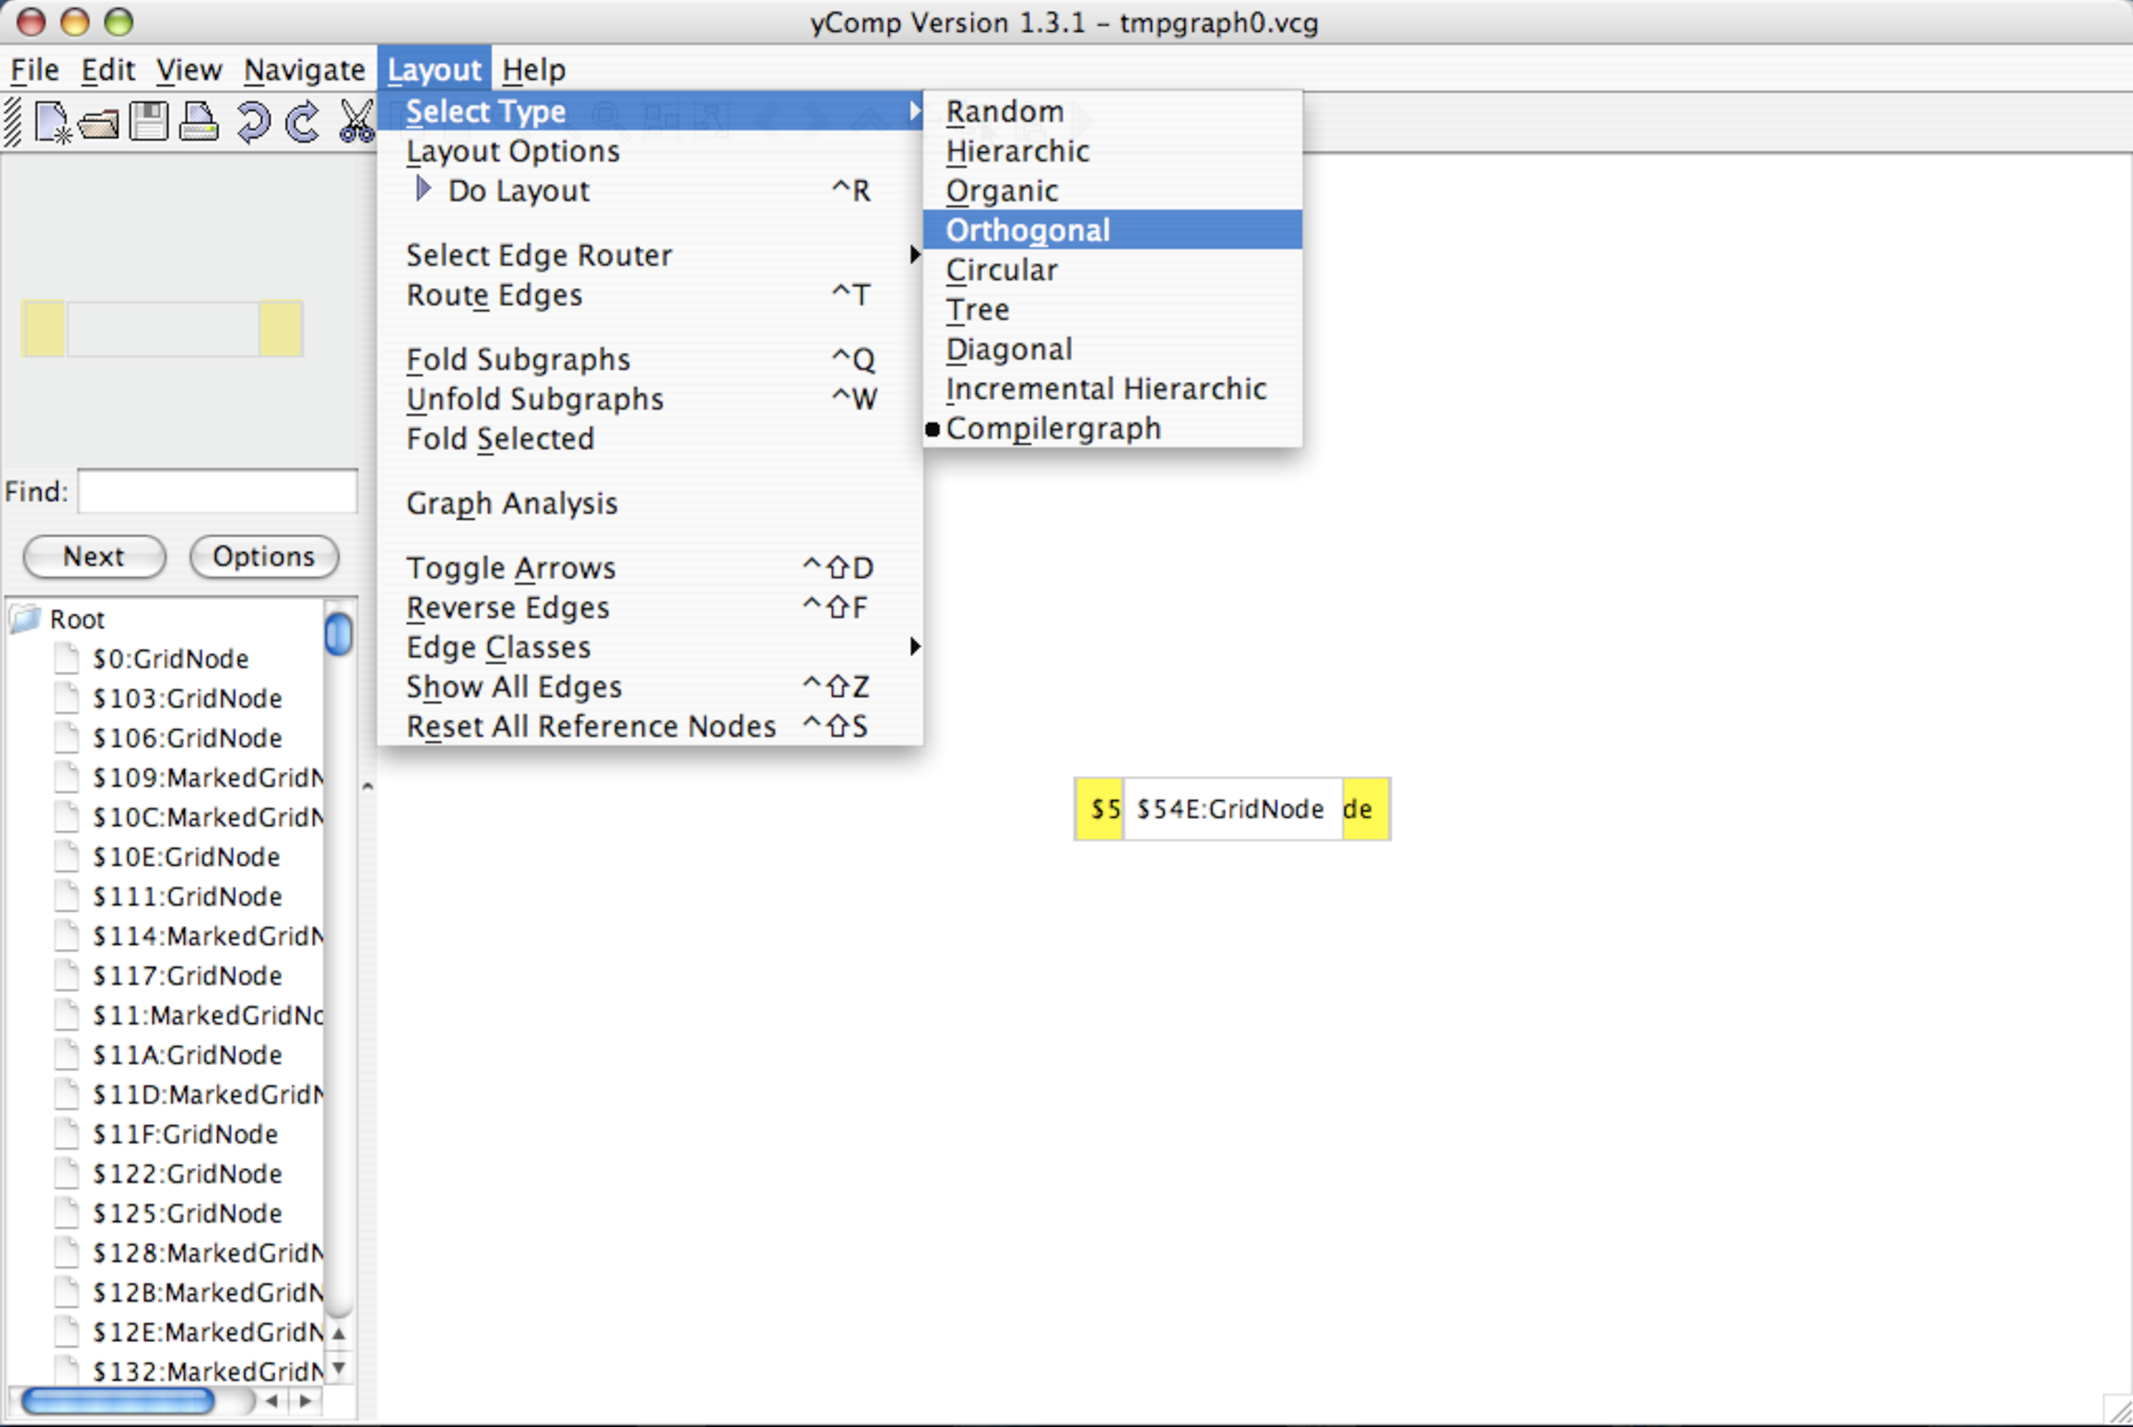
\includegraphics[width=0.45\linewidth]{fig/ycomp1.pdf} 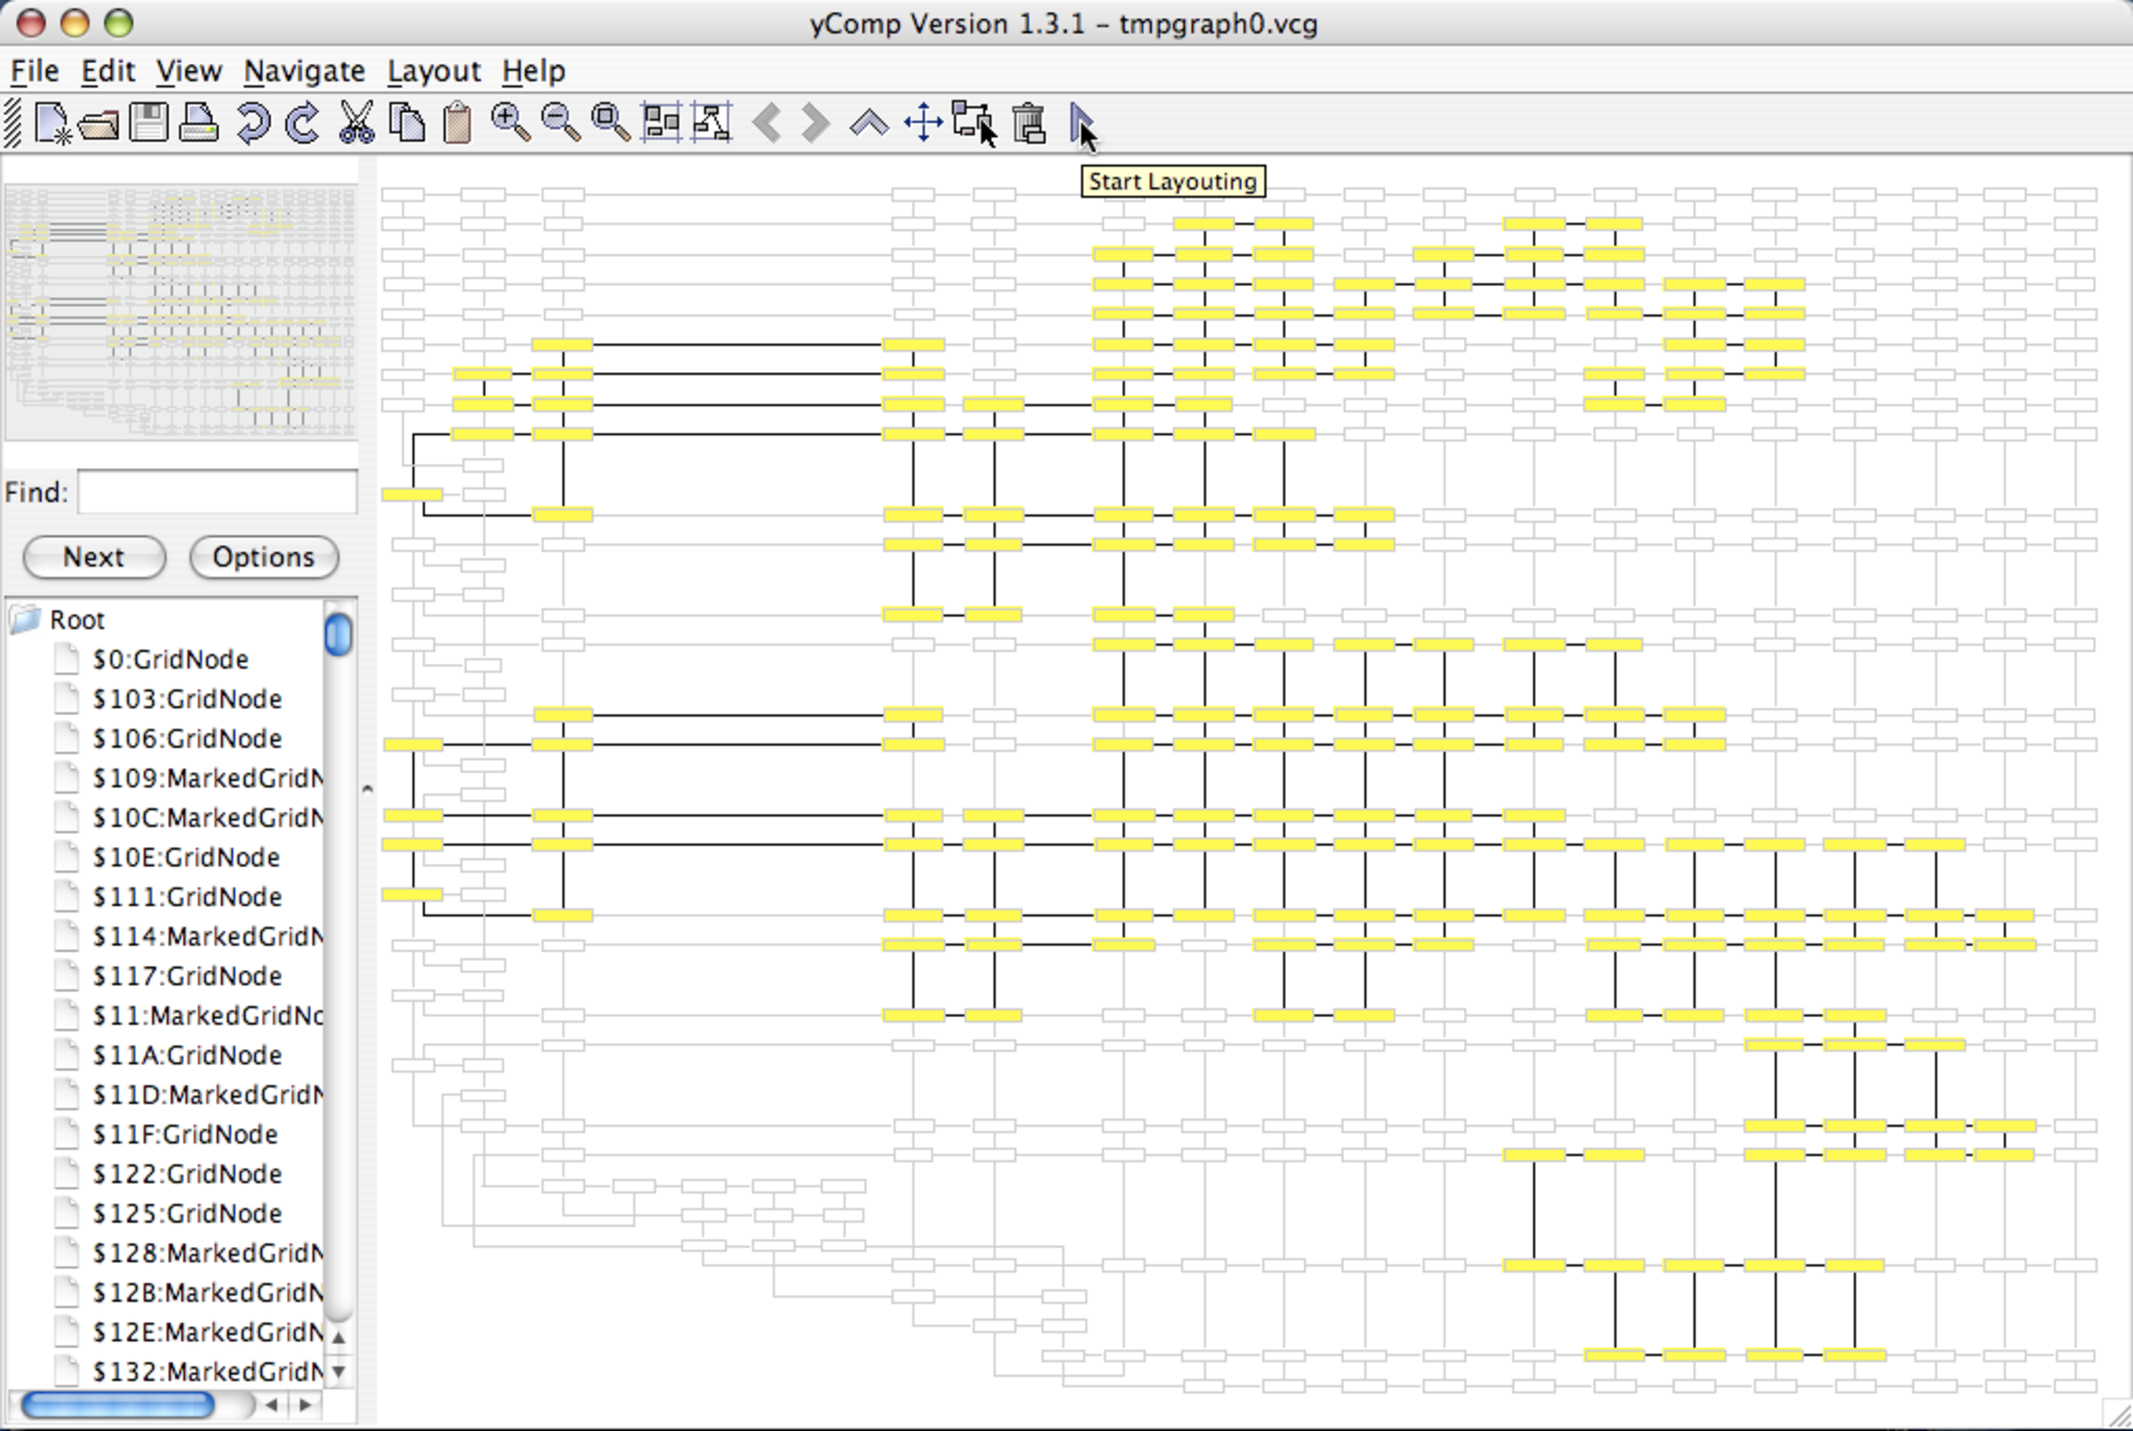
\includegraphics[width=0.45\linewidth]{fig/ycomp2.pdf}
\end{center}
  \item[Requires] Java Runtime Environment 1.5 (or above).
\end{description}




\chapter{Graph Model Language}
\label{chapmodellang}
The key features of \GrG\ graph models from \cite{geiss}:

\begin{description}
\item[Types.] Nodes and edges can have types (classes). This is similar to common programming languages, except \GrG\ types have no concept of methods. 
\item[Attributes.] Nodes and edges can possess attributes. The set of attributes assigned to a node or edge is determined by its type. The attributes themselves are typed, too.
\item[Inheritance.] Types (classes) can be composed by multiple inheritance. \emph{Node} and \emph{Edge} are built-in root types of node and edge types, respectively. Inheritance eases the specification of attributes, because subtypes inherit the attributes of their super types. Note that \GrG\ lacks a concept of overwriting. On a path in the type hierarchy graph from a type up to the built-in root type there must be exactly one declaration for each attribute identifier.
\item[Connection Assertions.] To specify that certain edge types should only connect specific nodes, we include connection assertions. Furthermore the number of outgoing and incoming edges can be constrained.
\end{description}

\begin{figure}[htbf]
\begin{example}\label{ex:model:map}
The following toy example of a model of street maps gives a rough picture of the language:
\begin{grgen}
model Map;

enum resident {village = 500, town = 5000, city = 50000}

node class sight;

node class city {
	size: resident;
}

const node class metropolis extends city {
  river: string;
}  

abstract node class abandoned_city extends city;
node class ghost_town extends abandoned_city;

edge class street;
edge class trail extends street;
edge class highway extends street
    connect metropolis [+] -> metropolis [+]
{
    jam: boolean;
}
\end{grgen}
\end{example}
\end{figure}
In this chapter as well as in the \GrShell\ chapter \ref{chapgrshell} we use excerpts of example~\ref{ex:model:map} (the \texttt{Map} model) for further descriptions.

\section{Building Blocks}
\label{modelbb}

\begin{note}
The following syntax specifications make heavy use of syntax diagrams (also known as rail diagrams). Syntax diagrams provide a visualization of EBNF\footnote{Extended Backus–Naur Form.} grammars. Follow a path along the arrows from left to right through a diagram to get a valid sentence (or sub sentence) of the language. Ellipses are terminals whereas rectangles are non-terminals. For further information on syntax diagrams see \cite{pascal}.
\end{note}
Basic elements of the \GrG\ graph model language are identifiers to denominate types, attributes, and the model itself. The \GrG\ graph model language is case sensitive.\\
\\
\emph{Ident}, \emph{IdentDecl}\\ \nopagebreak
A non-empty character sequence of arbitrary length consisting of letters, digits or underscores. The first character must not be a digit. \emph{Ident} and \emph{IdentDecl} differ in their role: While \emph{IdentDecl} is a \emph{defining} occurrence of an identifier, \emph{Ident} is a \emph{using} occurrence. An \emph{IdentDecl} non-terminal can be annotated. See \ref{annotations} for annotations of declarations.
\begin{note}
  The \GrG\ model language does not distinguish between declarations and definitions. More precisely, every declaration is also a definition. For instance, there are no C-like constructs as the following:
\begin{grgen}
node class t_node;
node class t_node {
}
\end{grgen}
\end{note}
\mbox{ }\\
\emph{NodeType}, \emph{EdgeType}, \emph{EnumType}\\ \nopagebreak
These are (semantic) specializations of Ident to restrict an identifier to be of a specific type.

\section{Type Declarations}
\begin{rail}
  GraphModel: 'model' IdentDecl ';' (() + TypeDeclaration);
\end{rail}
The graph model consists of its name \emph{IdentDecl} and type declarations defining specific node and edge types as well as enums.

\begin{rail}
  TypeDeclaration: EnumDeclaration | ClassDeclaration
\end{rail}
\emph{ClassDeclaration} defines a node or an edge. \emph{EnumDeclaration} defines an enum type for use as attribute of nodes or edges. Types do not need to be declared before they are used.

\begin{rail}
  EnumDeclaration: 'enum' IdentDecl lbrace ((IdentDecl (() | '=' IntExpr)) + ',') rbrace ;
\end{rail}
Defines an enum type.

\begin{example}
\begin{grgen}
enum Color {red, green, blue}
enum Resident {village = 500, town = 5000, city = 50000}
enum AsInC {a = 2, b, c = 1, d, e = Resident::village + c}
\end{grgen}
The semantics is as it is in C \cite{isoc}. So the following holds: $\text{red} = 0$, $\text{green} = 1$, $\text{blue} = 2$, $\texttt{a}=2$, $b=3$, $c=1$, $d=2$, and $e=501$.
\end{example}

\begin{rail}  
  ClassDeclaration: (() | 'abstract') (() | 'const') (NodeClass | EdgeClass);
\end{rail}
Defines a new node type or edge type.\\
The keyword \texttt{abstract} indicates that you cannot instantiate graph elements of this type but rather you have to derive non-abstract types for graph elements. The abstract-property will not be inherited by subclasses.

\begin{example}
We adjust our map model and make \texttt{city} abstract:
\begin{grgen}
abstract node class city {
	size: int;
}
abstract node class abandoned_city extends city;
node class ghost_town extends abandoned_city;
\end{grgen}
You will be able to create nodes of type \texttt{ghost\_town}, but not of type \texttt{city} or \texttt{abandoned\_city}. However, nodes of type \texttt{ghost\_town} are also nodes of type \texttt{abandoned\_city} and of type \texttt{city} and they have the attribute \texttt{size}.
\end{example}
The keyword \texttt{const} indicates that rules may not write to attributes. See also \ref{replacepart}, \texttt{eval}. However, attributes are writable by \LibGr\ and \GrShell\ directly. This property will not be inherited by subclasses. If you want a subclass to have constant attributes, you have to set the \texttt{const} modifier explicitly.

\begin{rail}  
  NodeClass: 'node' 'class' IdentDecl (() | 'extends' (NodeType+',')) \\ 
    (';' | lbrace AttributeDeclarations rbrace);
\end{rail}
Defines a new node type. Node types can inherit from other node types defined within the same file. If the \texttt{extends} clause is omitted, \emph{NodeType} will inherit from the built-in type \texttt{Node}. Optionally nodes can possess attributes.

\begin{rail}    
  EdgeClass: 'edge' 'class' IdentDecl (() | 'extends' (EdgeType+',')) \\
    (() + ConnectAssertions) (';' | lbrace AttributeDeclarations rbrace);
\end{rail}
Defines a new edge type. Edge types can inherit from other edge types defined within the same file. If the \texttt{extends} clause is omitted, \emph{EdgeType} will inherit from the built-in type \texttt{Edge}. Optionally edges can possess attributes. A \emph{connection assertion} specifies that certain edge types should only connect specific nodes and, moreover, the number of outgoing and incoming edges can be constrained.

\begin{rail}  
  ConnectAssertions: 'connect' (NodeConstraint '->' NodeConstraint + ',');
  NodeConstraint: NodeType (() | '[' ('*' | '+' | Number | RangeConstraint) ']') ;
  RangeConstraint: Number ':' ('*' | Number) ;
\end{rail}
A connection assertion is typed as a pair of node types in conjunction with their multiplicities. A corresponding edge may connect a node of the first node type or one of its subtypes (source) with a node of the second node type or one of its subtypes (destination). The multiplicity is a constraint on the out-degree and in-degree of the source and destination node type respectively. \emph{Number} is an \texttt{int} constant as defined in section \ref{expressions}. See \ref{graphcommands}, \texttt{validate}, for an example. Table \ref{multiplicities} describes the multiplicity definitions.
\begin{table}[htbp]
\begin{tabularx}{\linewidth}{|l|X|}\hline
	\texttt{[n:*]} & The number of edges nodes of that type are incident to is unbounded. At least $n$ edges must be incident to nodes of that type.\\ 
	\texttt{[n:m]} & At least $n$ edges must be incident to nodes of that type, but at most $m$ edges may be incident to nodes of that type ($m \geq n$ must hold).\\
	\texttt{[*]} & Abbreviation for \texttt{[0:*]}.\\
	\texttt{[+]} & Abbreviation for \texttt{[1:*]}\\
	\texttt{[n]} & Abbreviation for \texttt{[n:n]}. \\ \hline
\end{tabularx}
\caption{\GrG\ node constraint multiplicities concerning a specific pair of an edge type and a node type.}
\label{multiplicities}
\end{table}

\begin{rail}    
  AttributeDeclarations: (() | IdentDecl ':' AttributeType ';') + ;
  AttributeType: PrimitiveType | EnumType ; 
\end{rail}
Defines a node or edge attribute. Possible types are \texttt{enum} and primitive types. See \ref{builtin} for a list of built-in primitive types.




\chapter{Rule Set Language}\indexmain{rule set language}
\label{chaprulelang}

The \indexed{rule set} language forms the core of \GrG. Rule files refer to zero\footnote{Omitting a graph meta model means that \GrG\ uses a \indexed{default graph model}. The default model consists of the base type \texttt{Node} for vertices and the base type \texttt{Edge} for edges.} or more \indexed{graph model}s and specify a set of rewrite rules. The rule language covers the pattern specification and the replace/modify specification. Attributes of graph elements can be re-evaluated during an application of a rule. The following rewrite rule mentioned in Geiß et al.~\cite{GBGHS:06} gives a rough picture of the language:
%\begin{figure}[tb]
\begin{example}\label{ex:rule:SomeRule}
\begin{grgen}
using SomeModel;

rule SomeRule {
  n1:NodeTypeA;
  n2:NodeTypeA;
  hom(n1, n2);
  n1 --> n2; /*@\label{ex:somerule:graphlet}@*/
  n3:NodeTypeB;
  negative {
    n3 -e1:EdgeTypeA-> n1;
    if {n3.a1 == 42*n2.a1;}
  }
  negative { /*@\label{ex:somerule:secondnac:begin}@*/
    n4:Node\(NodeTypeB);
    n3 -e1:EdgeTypeB-> n4;
    if {typeof(e1) >= EdgeTypeA;}
  } /*@\label{ex:somerule:secondnac:end}@*/
  replace {
    n5:NodeTypeC<n1>;
    n3 -e1:EdgeTypeB-> n5;
    eval {n5.a3 = n3.a1*n1.a2;}
  }  
}
\end{grgen}
\end{example}
%\end{figure}
In this chapter we use excerpts of Example~\ref{ex:rule:SomeRule} (\texttt{SomeRule}) for illustration purposes.
The nested negative which specify a pattern which must not be available in the host graph are described in the following chapter \ref{cha:nestedsub}

\section{Building Blocks}
\label{rulebb}

The \GrG\ rule set language is \indexed{case sensitive}. The language makes use of several identifier specializations in order to denominate all the \GrG\ entities.\\
\\
\emph{Ident}, \emph{IdentDecl}\\ \indexmain{identifier}\nopagebreak
A non-empty character sequence of arbitrary length consisting of letters, digits, or underscores. The first character must not be a digit. \emph{Ident} may be an identifier defined in a graph model (see Section~\ref{modelbb}). \emph{Ident} and \emph{IdentDecl} differ in their role: While \emph{IdentDecl} is a \emph{defining} occurrence of an identifier, \emph{Ident} is a \emph{using} occurrence. An \emph{IdentDecl} non-terminal can be annotated\indexmain{annotation}. See Section~\ref{annotations} for annotations of declarations.
\begin{note}
  As in the \GrG\ model language (see note~\ref{note:modeldecl}) every declaration is also a definition. Using an identifier before defining it is allowed. Every used identifier has to be defined exactly once.
\end{note}
\mbox{ }\\
\emph{ModelIdent}, \emph{TypeIdent}, \emph{NodeType}, \emph{EdgeType}\\
These are (semantic) specializations of \emph{Ident}. \emph{TypeIdent} matches every type identifier, i.e.\ a node type, an edge type, an enumeration type or a primitive type. All the type identifiers are actually type \emph{expressions}\indexmain{type expression}. See Section~\ref{typeexpressions} for the use of type expressions.\\

\subsection{Graphlets}
\label{sct:graphlets}
\begin{rail}
  Graphlet: (GraphletNode (() | Continuation) | Continuation) ';' ;
  Continuation: GraphletEdge (() | (GraphletNode (() | Continuation))) ;
\end{rail}\ixnterm{Graphlet}\ixnterm{Continuation}
A \indexed{graphlet} specifies a connected subgraph. 
\GrG\ provides graphlets as a descriptive notation to define both, patterns\indexmain{pattern graph} to search for as well as the subgraphs that replace or modify matched \indexed{spot}s in a host graph\indexmain{replacement graph}. 
Any graph can be specified piecewise by a set of graphlets. 
In Example~\ref{ex:rule:SomeRule}, line~\ref{ex:somerule:graphlet}, the statement \texttt{n1 --> n2} is the node identifier \texttt{n1} followed by the \indexedsee{continuation}{graphlet} graphlet \texttt{--> n2}.

All the graph elements of a graphlet have \newterm{name}s.
The name is either user-assigned or a unique internal, non-accessible name.
In the second case the graph element is called \newterm{anonymous}.
For illustration purposes we use a \indexed{\texttt{\$<number>}} notation to denote anonymous graph elements in this document.
For example the graphlet \texttt{n1 --> n2} contains an anonymous edge; thus can be understood as \texttt{n1 -\$1:Edge-> n2}.
Names must not be \indexed{redefine}d; once defined, a name is \emph{bound} to a graph element. 
We use the term ``\indexed{binding of names}'' because a name not only denotes a graph element of a graphlet but also denotes the mapping of the abstract graph element of a graphlet to a concrete graph element of a host graph.
So graph elements of different names are pair wise distinct except for homomorphically matched\indexmain{homomorphic matching} graph elements (see Section~\ref{patternpart}).
For instance \texttt{v:NodeType1 -e:EdgeType-> w:NodeType2} selects some node of type \texttt{Node\-Type1} that is connected to a node of type \texttt{NodeType2} by an edge of type \texttt{EdgeType} and binds the names \texttt{v}, \texttt{w}, and \texttt{e}. 
If \texttt{v} and \texttt{w} are not explicitly marked as homomorphic, the graph elements they bind to are distinct.
Binding of names allows for splitting a single graphlet into multiple graphlets as well as defining cyclic structures.
\begin{example}
The following graphlet (\texttt{n1}, \texttt{n2}, and \texttt{n3} are defined somewhere else)
\begin{grgen}
n1 --> n2 --> n3 <-- n1;
\end{grgen}
is equivalent to
\begin{grgen}
n2 --> n3;
n1 --> n2;
n3 <-- n1;
\end{grgen}
and \texttt{n1 --> n3} is equivalent to \texttt{n3 <-- n1}, of course.
\end{example}
The visibility of names is determined by \indexed{scope}s. 
Scopes can be nested. 
Names of surrounding scopes are visible in inner scopes. 
Usually a scope is defined by \texttt{\{} and \texttt{\}}. %In contrast to pure syntactic scoping, the replace/modify part is a direct inner scope of the pattern part.
In Example~\ref{ex:rule:SomeRule}, lines~\ref{ex:somerule:secondnac:begin}~to~\ref{ex:somerule:secondnac:end}, the negative condition uses \texttt{n3} from the surrounding scope and defines \texttt{n4} and \texttt{e1}. 
We may safely reuse the variable name \texttt{e1} in the replace part.

\begin{rail}
GraphletNode: (Ident | 
    '.' |
    (() | IdentDecl) ':' NodeType (() | TypeConstraint | Retyping)) ;   
\end{rail}\ixnterm{GraphletNode}
Specifies a node\indexmain{node (graphlet)} of type \emph{NodeType},
maybe constrained in type with a \emph{TypeConstraint}\indexmain{type constraint} (see Section~\ref{typehandling}, \emph{TypeConstraint}),
maybe retyped with a \emph{Reytping}\indexmain{retype} (see Section~\ref{typehandling}, \emph{Retyping}).
The \texttt{.}\ is an anonymous node of the base type \texttt{Node}; remember that every node type has \texttt{Node} as super type. 
Type constraints are allowed in the pattern part only. 
Retyping is allowed in the replace/modify part only.
\begin{center}
  \begin{tabularx}{\linewidth}{lX}
    \textbf{Graphlet} & \textbf{Meaning}\\ \hline
    \texttt{x:NodeType;} & The name \texttt{x} is bound to a node of type \texttt{NodeType} or one of its subtypes. \\
    \texttt{ :NodeType;} & \texttt{\$1:NodeType} \\
    \texttt{.;} & \texttt{\$1:Node} \\
    \texttt{x;} & The node, \texttt{x} is bound to.
  \end{tabularx}
\end{center} 

\begin{rail}
  GraphletEdge: '-' EdgeRefinement '->'  | '<-' EdgeRefinement '-'  | '<-' EdgeRefinement '->' | '?-' EdgeRefinement '-?' ;
  EdgeRefinement: () | Ident | (() | IdentDecl) ':' EdgeType (() | TypeConstraint | Retyping) ;
\end{rail}\ixnterm{GraphletEdge}\ixnterm{EdgeRefinement}
A \emph{GraphletEdge} specifies an edge\indexmain{edge (graphlet)}. 
Anonymous edges are specified by an empty \emph{EdgeRefinement} clause, i.\,e.\ \texttt{-->}, \texttt{<--}, \texttt{<-->}, \texttt{--}, \texttt{?--?} or \texttt{-:T->}, \texttt{<-:T-}, \dots\ for an edge type \texttt{T}, respectively. 
A non-empty \emph{EdgeRefinement} clause allows for detailed edge type specification. 
Type constraints\indexmain{type constraint} are allowed in the pattern part only (see Section~\ref{typehandling}, \emph{TypeConstraint}).
Retyping is allowed in the replace/modify part only (see Section~\ref{typehandling}, \emph{Retyping}).

The different kind of arrow tips distinguish between \indexed{directed}, \indexed{undirected}, and \indexed{arbitrary} edges (see also Section~\ref{sct:basetypes}).
The arrows \texttt{-->} and \texttt{<--} are used for directed edges with a defined source and target.
The arrow \texttt{--} is used for undirected edges.
The pattern part allows for further arrow tips, namely \texttt{?--?}\ for arbitrary edges and \texttt{<-->} for directed edges with undefined direction.
Note that \texttt{<-->} is \emph{not} equivalent to the \texttt{--> ; <-- ;} statements.
In order to produce a match for the arrow \texttt{<-->}, it is sufficient that one of the statements \texttt{-->}, \texttt{<--} matches.
If an edge type is specified (through the \emph{EdgeRefinement} clause), this type has to correspond to the arrow tips, of course.
\begin{center}
	\begin{tabularx}{\linewidth}{lX}
		\textbf{Graphlet} & \textbf{Meaning}\\ \hline
		\texttt{ -e:EdgeType-> ;} & The name \texttt{e} is bound to an edge of type \texttt{EdgeType} or one of its subtypes. \\
		\texttt{ -:EdgeType-> ;} & \texttt{-\$1:EdgeType-> ;} \\
		\texttt{ --> ;} & \texttt{-\$1:Edge-> ;} \\
		\texttt{ <--> ;} & \texttt{-\$1:Edge-> ;} or  \texttt{<-\$1:Edge- ;}\\
		\texttt{ -- ;} & \texttt{-\$1:UEdge-> ;} \\
		\texttt{ ?--?\ ;} & \texttt{-\$1:AEdge-> ;} \\
		\texttt{ -e-> ;} & The edge, \texttt{e} is bound to.
	\end{tabularx}
\end{center} 
As the above table shows, edges can be defined and used separately, i.e.\ without their incident nodes. Beware of accidentally ``\indexed{redirecting}''\footnote{You cannot directly express the redirection of edges. This a direct consequence of the \indexedsee{SPO}{single-pushout approach}\indexmain{single-pushout approach} approach. Redirection of edges can be ``simulated'' by either deleting and re-inserting an edge, or more indirect by re-typing of nodes.} an edge: 
The graphlets
\begin{grgenlet}
-e:Edge-> .;
x:Node -e-> y:Node;
\end{grgenlet}
are illegal, because the edge \texttt{e} would have two destinations: an anonymous node and \texttt{y}.
However, the graphlets
\begin{grgenlet}
-e-> ;
x:Node -e:Edge-> y:Node;
\end{grgenlet}
are allowed, but the first graphlet \texttt{-e->} is superfluous. In particular this graphlet does not identify or create any ``copies'', neither if the graphlet occurs in the pattern part nor if it occurs in the replace part.
\begin{example}
Some attempts to specify a loop edge:\\
\mbox{ }\\
\begin{tabular}[c]{ll} 
 \textbf{Graphlet} & \textbf{Meaning} \\ \hline
 \texttt{x:Node -e:Edge-> x;} & The edge \texttt{e} is a loop.\\ 
 \texttt{x:Node -e:Edge-> ; -e-> x;} & The edge \texttt{e} is a loop.\\ 
 \texttt{-e:Edge-> x:Node;} & The edge \texttt{e} may or may not be a loop.\\ 
 \texttt{.\ -e:Edge-> .;} & The edge \texttt{e} is certainly not a loop.\\ 
\end{tabular}
\end{example}

\begin{figure}[htbp]
\begin{example}
\label{ex:somegraphlets}
Some graphlets:

\begin{center}
\begin{tabular}[c]{cl}
  & \\
  \begin{tabular}[c]{c}\begin{tikzpicture}
      \tikzstyle{every node}=[circle]
      \node[draw] (n1) at (1,0) {};
      \node[draw] (n2) at (2,1) {};
      \node[draw] (n3) at (1,2) {};
      \node[draw] (n4) at (0,1) {};
    	
      \draw[-latex] (n3) .. controls +(-1,0) .. (n4) {};
      \draw[-latex] (n4) .. controls +(0,-1) .. (n1) {};
      \draw[-latex] (n1) .. controls +(1,0) .. (n2) {};
      \draw[-latex] (n2) .. controls +(0,1) .. (n3) {};
    \end{tikzpicture}\end{tabular} & \begin{tabular}[c]{l} \texttt{x:Node --> .\ --> .\ --> .\ --> x;} \end{tabular}\\
  & \\  
  \begin{tabular}[c]{c}\begin{tikzpicture}
      \tikzstyle{every node}=[circle]
      \node[draw] (n1) at (1,1) {};
      \node[draw] (n2) at (0,0) {};
      \node[draw] (n3) at (0,2) {};
      \node[draw] (n4) at (2,0) {};
      \node[draw] (n5) at (2,2) {};
    	
      \draw[-latex] (n1) -- (n2) {};
      \draw[-latex] (n1) -- (n3) {};
      \draw[-latex] (n1) -- (n4) {};
      \draw[-latex] (n1) -- (n5) {};
    \end{tikzpicture}\end{tabular} & \begin{tabular}[c]{l} \texttt{.\ <-- x:Node --> .;} \\ \texttt{.\ <-- x --> .;} \end{tabular}\\
  & \\
  \begin{tabular}[c]{c}\begin{tikzpicture}
      \tikzstyle{every node}=[circle]
      \node[draw] (n1) at (3,5) {};
      \node[draw] (n2) at (2,4)   {};
      \node[draw] (n3) at (0,2)   {};
      \node[draw] (n4) at (2,0)   {};
      \node[draw] (n5) at (4,2)   {};
      \node[draw] (n6) at (2,5.0)   {};
    	
    	\draw[-latex] (n2) --                                  (n1) node[right,pos=0.6] {$e_1:\text{stem}$};
    	\draw[-latex] (n2) .. controls +(-1,1) and +(0,1) ..   (n3) node[left,midway]  {$e_2$};
      \draw[-latex] (n3) .. controls +(0,-1) and +(-1,0) ..  (n4) node[left,midway]  {$e_3$};
    	\draw[-latex] (n4) .. controls +(1,0)  and +(0,-1) ..  (n5) node[right,midway] {$e_4$};
      \draw[-latex] (n5) .. controls +(0,1)  and +(1,1) ..   (n2) node[right,midway] {$e_5$};
    	\draw[-latex] (n2) .. controls +(-0.3,+0.3) and +(-0.3,-0.3) .. (n6) node[left,midway]   {};
    	\draw[-latex] (n2) .. controls +(+0.3,+0.3) and +(+0.3,-0.3) .. (n6) node[right,midway]  {};
    \end{tikzpicture}\end{tabular} & \begin{tabular}[c]{l} \texttt{.\ <-e1:stem- n1:Node -e2:Edge-> .\ -e3:Edge-> .} \\ \quad\texttt{-e4:Edge-> .\ -e5:Edge-> n1;}\\ \texttt{n1 --> n2:Node;} \\ \texttt{n1 --> n2;} \end{tabular}\\
   & \\
  \begin{tabular}[c]{c}\begin{tikzpicture}
      \tikzstyle{every node}=[circle]
      \node[draw] (n1) at (0,0) {};
      \node[draw] (n2) at (1,0) {};
      \node[draw] (n3) at (2,0) {};
      \node[draw] (n4) at (3,0) {};
      \node[draw] (n5) at (4,0) {};
    	
      \draw[-latex] (n1) -- (n2) {};
      \draw[-latex] (n3) -- (n2) {};
      \draw[-latex] (n4) -- (n3) {};
      \draw[-latex] (n4) -- (n5) {};
    \end{tikzpicture}\end{tabular} & \begin{tabular}[c]{l} \texttt{.\ --> .\ <-- .\ <-- .\ --> .;} \end{tabular} \\
  & \\
  \begin{tabular}[c]{c}\begin{tikzpicture}
      \tikzstyle{every node}=[circle]
      \node (n1) at (0,0) {};
      \node[draw] (n2) at (1,0) {};
      \node[draw] (n3) at (2,0) {};
      \node (n4) at (3,0) {};
    	
      \draw[-latex] (n2) -- (n1) {};
      \draw[-latex] (n3) -- (n2) node[midway,above] {$e$};
      \draw[-latex] (n3) -- (n4) {};
    \end{tikzpicture}\end{tabular} & \begin{tabular}[c]{l} \texttt{-e:Edge->} \\ \texttt{<-- .\ <-e- .\ -->\ ;} \end{tabular}
\end{tabular}\\
\end{center}
\mbox{ }\\
\mbox{ }\\
\mbox{ }\\
And some illegal graphlets:\\
\mbox{}\\
\mbox{}\\
\begin{tabularx}{\linewidth}{cX}
\texttt{.\ -e:Edge-> .; .\ -e-> .;} & Would affect redirecting of edge \texttt{e}. \\
 & \\
 \texttt{x -e:T-> y; x -e-> x;} & Would affect redirecting of edge \texttt{e}. \\
 & \\
 \texttt{<-- --> ;} & There must be at least a node between the edges.
\end{tabularx}
\end{example}
\end{figure}

\begin{note}
	Although both, the pattern part and the replace/modify part use graphlets, there are subtle differences between them. 
	These concern the \emph{TypeConstraint} and \emph{Retyping} clause plus the allowed arrow tips for edges.
\end{note}

\section{Rules and Tests}
\label{ruledecls}
The structure of a \indexed{rule set} file is as follows:
\begin{rail}
  RuleSet: Header ((TestDeclaration | RuleDeclaration | SubpatternDeclaration)+) ;
  Header: ('using' ((ModelIdent)+',') ';')? (('\#include' Filename)*());
\end{rail}\ixkeyw{using}\ixnterm{RuleSet}

A rule set consists of the underlying \indexed{graph model}s and several rewrite rules and tests (subpatterns will be introduced in \ref{sec:subpattern}).
Additionally you may include further rule set files (without \texttt{using} directives, we prefer to suffix them with \textt{.gri} in this case).
In case of multiple graph models, \GrG\ uses the union of these models. In this case beware of conflicting declarations.
There is no built-in conflict resolution mechanism like packages or namespaces for models.
If necessary you can use prefixes as you might do in C.

\begin{rail}
  TestDeclaration: 'test' (() | 'exact' | 'induced') ActionSignature lbrace Pattern rbrace ;
  RuleDeclaration: 'rule' (() | 'exact' | 'induced' | 'dpo') ActionSignature lbrace Pattern Replace rbrace ;
\end{rail}\ixkeyw{test}\ixkeyw{rule}\ixkeyw{exact}\ixkeyw{induced}\ixkeyw{dpo}\ixnterm{TestDeclaration}\ixnterm{RuleDeclaration}
Declares a single \indexed{rewrite rule} such as \texttt{SomeRule}. 
It consists of a pattern part (see Section~\ref{patternpart}) in conjunction with its rewrite/modify part (see Section~\ref{replacepart}). 
A \newterm{test} has no rewrite specification. 
It's intended to check whether (and maybe how many times) a pattern occurs (see example \ref{ex:rulelang:testrule}).
For an explanation of the \texttt{exact}, \texttt{induced}, and \texttt{dpo} pattern modifiers see section \ref{sct:patternmodifier}. 
\begin{example}
\label{ex:rulelang:testrule}
We define a test \texttt{SomeCond}
\begin{grgen}
test SomeCond {
  n:SeldomNodeType;
}
\end{grgen}
and execute in \GrShell:
\begin{grshell}
  grs SomeCond & SomeRule
\end{grshell}
SomeRule will only be executed, if a node of type \texttt{SeldomNodeType} exists. 
For graph rewrite sequences in \GrShell\ see Section~\ref{grsthings}.
\end{example}

\begin{rail}  
  ActionSignature: IdentDecl (() | Parameters) (() | ':' ReturnTypes) ;
\end{rail}\ixnterm{ActionSignature}
The \indexed{signature} sets the name of a rewrite rule to \emph{IdentDecl} and optionally names and types of formal \indexed{parameter}s as well as a list of \indexed{return type}s.
Parameters and return types provide users with the ability to exchange graph elements between rules, similar to parameters of procedural languages.
This way it is possible to specify \emph{where} a rule should be applied.

\begin{rail}
  Parameters: '(' (Parameter * ',') ')' ;
  Parameter: IdentDecl ':' NodeType (InputTypeSpecification)? | '-' IdentDecl ':' EdgeType (InputTypeSpecification)? '->' | 'var' IdentDecl ':' VarType ;
  InputTypeSpecification: '<' (NodeEdgeType | 'null' | NodeEdgeType '+' 'null' | 'null' '+' NodeEdgeType ) '>' ;
\end{rail}\ixnterm{Parameters}

Within a rule, graph element parameters are treated as graph elements of the pattern - just predefined.
But in contrast to pervious versions it is the task of the user to ensure the elements handed in satisfy the interface, i.e. parameters must not be null and must be of the type specified or a subtype of the type specified. 
If you need more flexibility and want to call the rule with parameters not fullfilling the interface you can append an input type specification to the relevant parameters, which consists of the type to accept at the action interface, or null, or both, enclosed in left and right angles. 
If the input type specification type is given, but the more specific pattern element type is not satisfied, matching simply fails.
If null is declared in the input type specification and given at runtime, the element is searched in the host graph.
Don't use null parameters unless you need them, because every null parameter doubles the number of matcher routines which get generated.
Non-graph element parameters must be prefixed by the \texttt{var}-keyword, VarType is one of the attribute types supported by \GrG (\ref{built-in-types}).
Please not that the effect of assigning to a var parameter in \texttt{eval}\ref{eval} is undefined (concerning the parameters as well as the argument).

\begin{figure}[htbp]
\begin{example}
The \indexed{test} \texttt{t} that checks whether node \texttt{n1} is \indexed{adjacent} to \texttt{n2} (connected by an undirected edge or incoming directed edge or outgoing directed edge)
\begin{grgen}
test t(n1:Node<null>, n2:Node<null>) {
  n1 ?--? n2;
}
\end{grgen}
is equivalent to the tests \texttt{t1}-\texttt{t4} which are chosen dependent on what parameters are defined.
\begin{grgen}
test t1(n1:Node, n2:Node) {
  n1 ?--? n2;
}
test t2(n1:Node) {
  n1 ?--? n2:Node;
}
test t3(n2:Node) {
  n1:Node ?--? n2;
}
test t4 {
  n1:Node ?--? n2:Node;
}
\end{grgen}
So if both parameters are not defined, \texttt{t4} is chosen, which succeeds as soon as there are two distinct nodes in the graph connected by some edge.
\end{example}
\end{figure}

\begin{rail}
  ReturnTypes: '(' ((NodeType | EdgeType | VarType) + ',') ')' ;
\end{rail}\ixnterm{ReturnTypes}
The return types specify edge and node types of graph elements that are returned by the replace/modify part. If return types are specified, the \texttt{return} statement is mandatory. Otherwise no \texttt{return} statement must occur. See also Section~\ref{replacepart}, \texttt{return}.

\begin{figure}[htbp]
\begin{example}\label{ex:rule:someruleext}
We extend \texttt{SomeRule} (Example~\ref{ex:rule:SomeRule}) with a user defined node to match and we want it to return the rewritten graph elements \texttt{n5} and \texttt{e1}.
\begin{grgen}
  rule SomeRuleExt(varnode:Node):(Node, EdgeTypeB) {
    n1:NodeTypeA;
    ...
    
    replace {
      varnode;
      ...  
      return(n5, e1);
      eval {
        ...
\end{grgen}
We do not define \texttt{varnode} within the pattern part because this is already covered by the parameter specification itself.
\end{example}
\end{figure}

\section{Pattern Part}\indexmain{pattern}
\label{patternpart}
%\begin{rail}
%  Pattern: (() + ('exact' | 'induced')) 'pattern' lbrace (()+PatternStatement) rbrace ;
%\end{rail}\ixkeyw{pattern}\ixkeyw{induced}\ixnterm{Pattern}
\begin{rail}
  Pattern: (()+PatternStatement) (() | ReturnStatement);
\end{rail}
A \indexed{pattern} consists of zero or more pattern statements and, in case of a test, an optional return statement.
All the pattern statements must be fulfilled by a subgraph of the host graph in order to form a match. 
An \indexed{empty pattern} always produces exactly one (empty) match. 
This is caused by the uniqueness of the total and totally undefined function.
For an explanation of the pattern modifiers \texttt{dpo}, \texttt{induced}, and \texttt{exact} see section~\ref{sct:patternmodifier}.

Names defined for graph elements may be used by other pattern statements as well as by replace/modify statements. 
Like all identifier definitions, such names may be used before their \indexed{declaration}. 
See Section~\ref{rulebb} for a detailed explanation of names and graphlets.
\begin{figure}[htbp]
\begin{note}
\label{note:indeterminism}
The \indexed{application} of a rule is not deterministic\indexmain{non-determinism}\indexmainsee{determinism}{non-determinism} (remember the example of the introduction in Section~\ref{ov:example}); in particular there may be more than one subgraph that matches the pattern. 
Whereas the \GrShell\ selects one of them arbitrarily (without further abilities to control the selection), the underlying \LibGr\indexmain{libGr} provides a mechanism to deal with such ambiguities. 

Also notice that graph rewrite \emph{sequences}\indexmain{graph rewrite sequence} introduce a further variant of non-determinism on rule application level: 
The \indexed{\texttt{\$<op>}} flag marks the operator \texttt{<op>} as commutative, i.e.\ the execution order of its operands (rules) is non-deterministic. 
See chapter~\ref{cha:xgrs} for further information on graph rewrite sequences.
\end{note}
\end{figure}

\begin{rail}  
  PatternStatement: 
    Graphlet ';' |
    'hom' '(' (Ident + ',') ')' ';' |
    ('exact' | 'induced') '(' (Ident+',') ')' |
    'if' lbrace (BooleanExpr ';' +) rbrace |
    NestedPattern |
    SubpatternEntityDeclaration
    ;

\end{rail}\ixkeyw{induced}\ixkeyw{exact}\ixkeyw{hom}\ixkeyw{if}\ixnterm{PatternStatement}
The semantics of the various pattern statements are given below:
\begin{description}
  \item[Graphlet] \indexmain{graphlet}Graphlets specify connected subgraphs. See Section~\ref{rulebb} for a detailed explanation of graphlets.
  \item[Isomorphic/Homomorphic Matching] \indexmain{isomorphic matching}\indexmain{homomorphic matching}The \texttt{hom} operator specifies the nodes or edges that may be matched homomorphically. 
  In contrast to the default isomorphic matching, the specified graph elements \emph{may} be mapped to the same graph element in the host graph. Note that the graph elements must have a common subtype. 
  Several homomorphically matched graph elements will be mapped to a graph element of a common subtype.
  In Example~\ref{ex:rule:SomeRule} nodes \texttt{n1} and \texttt{n2} may be the same node. This is possible because they are of the same type (\texttt{NodeTypeA}).
  Inside a NAC the \texttt{hom} operator may only operate on graph elements that are either defined or used in the NAC.
  Nested \texttt{negative}/\texttt{independent} blocks inherit the \texttt{hom} declarations of their nesting pattern.
  In contrast to previous versions \texttt{hom} delarations are non-transitive, i.e \texttt{hom(a,b)} and \texttt{hom(b,c)} don't cause \texttt{hom(a,c)} unless specified.
  \item[Attribute Conditions] \indexmain{attribute condition}The Java-like attribute conditions (keyword \texttt{if}) in the pattern part allow for further restriction of the applicability of a rule.
  \item[Pattern Modifiers] Additionally to modifiers that apply to a pattern as a whole, you may also specify pattern modifiers for a specific set of nodes. Accordingly the list of identifiers for a pattern modifier must not contain any edge identifier. See section \ref{sct:patternmodifier} for an explanation of the \texttt{exact} and \texttt{induced} modifiers. 
  \item[NestedPattern] will be explained in \ref{nac},\ref{pac},\ref{cardinality},\ref{alternative}.
  \item[SubpatternEntityDeclaration] will be explained in \ref{sec:subpattern}.
\end{description}

Keep in mind that using type constraints or the \texttt{typeof} operator might be helpful. See Section~\ref{typeexpressions} for further information.


\begin{rail}
  ReturnStatement: 'return' '(' ((Ident|Expression)+',') ')' ';' ;
\end{rail}\ixkeyw{return}\ixnterm{ReturnStatement}
\indexmain{return value}Returned graph elements (given by their name) and value entities (given by an expression computing them) must appear in the same order as defined by the return types in the signature (see Section~\ref{ruledecls}, \texttt{ActionSignature}).
Their types must be compatible to the return types specified.

\begin{note}
If you are using a graph at the API level without shell-provided names accessible by the \texttt{nameof}-operator, you may want to number the graph elements for dumping like this:
\begin{grgen}
rule numberNode(var id:int) : (int)
{
  n:NodeWithIntId;
  if { n.id == 0; }
  
  modify {
    eval {
      n.id = id;
    }
    return (id + 1);
  }
}
\end{grgen}
\end{note} 


\section{Replace/Modify Part}\indexmain{replacement graph}
\label{replacepart}
Besides specifying the pattern, a main task of a rule is to specify the transformation of a matched subgraph within the \indexed{host graph}. 
Such a \indexed{transformation specification} defines the transition from the \indexed{left hand side} (LHS) to the \indexed{right hand side} (RHS), i.e.\ which graph elements of a match will be kept, which of them will be deleted and which graph elements have to be newly created.

\subsection{Implicit Definition of the Preservation Morphism\indexmain{preservation morphism} $r$}
\label{rule:morphismr}
In theory the transformation specification is done by defining the preservation morphism $r$.
\begin{figure}[htbp]
	\centering
  \begin{tikzpicture}
    \begin{scope}[minimum size=0.5cm]
      \tikzstyle{every node}=[draw]
      \node (L)     at (0   ,2.5) {$L$};
      \node (R)     at (7   ,2.5) {$R$};
      \node (mL)    at (0   ,0) {};
      \node (mR)    at (7   ,0) {};
      \node[text width=2cm,text badly ragged,minimum size=1cm] (H)     at (0   ,0) {$H$};
      \node[text width=2cm,text badly ragged,minimum size=1cm] (Hs)    at (7   ,0) {$H'$};
    \end{scope}

    \draw[dotted,->] (L) node[above=0.4cm] {Pattern Graph} -> (mL) node[left,midway]  {Match $m$}   node[below=0.6cm] {Host Graph};
    \draw[dotted,->] (R) node[above=0.4cm] {Rewrite Graph} -> (mR)                              node[below=0.6cm] {Result Graph};

    \pgfsetshortenstart{0.5cm}
    \pgfsetshortenend{0.5cm}
    \draw[thick,->]  (L) -> (R)  node[above,midway] {Preservation Morphism $r$} node[below,midway] {Rule};
    \draw[thick,->]  (H) -> (Hs) node[below,midway] {Rule Application};
  \end{tikzpicture}
  \caption{Process of Graph Transformation}
  \label{rule:figrule}
\end{figure}
In \GrG\, the preservation morphism $r$ is defined implicitly by using \indexed{name}s both in pattern \indexed{graphlet}s and replace graphlets.
Remember that to each of the graph elements a name is bound to, either user defined or internally defined. If such a name is used in a replace graphlet, the denoted graph element will be kept. 
Otherwise the graph element will be deleted.
By defining a name in a replace graphlet a corresponding graph element will be newly created.
So in a replace pattern \indexed{anonymous} graph elements will always be created.
Using a name multiple times has the same effect as a single using occurrence.
In case of a conflict between \indexed{deletion} and \indexed{preservation}, deletion is prioritized. 
If an incident node of an edge gets deleted, the edge will be deleted as well (in compliance to the SPO\indexmain{single-pushout approach} semantics).

\begin{table}[htbp]
\centering
\begin{tabularx}{\linewidth}{lllX}
  \textbf{Pattern (LHS)} & \textbf{Replace (RHS)} & \textbf{$r: L \longrightarrow R$} & \textbf{Meaning} \\ \hline 
  \texttt{x:T;} & \texttt{x;}                 & $r:\lhs.x \mapsto \rhs.x$ & Preservation \\
  \texttt{x:T;} & \texttt{}                   & $\lhs.x \notin \deF(r)$    & Deletion \\
  \texttt{} & \texttt{x:T;}                   & $\rhs.x \notin \ran(r)$    & Creation \\
  \texttt{x:T;} & \texttt{x:T;}               & --- & Illegal, redefinition of \texttt{x} \\
  \texttt{-e:T-> ;} & \texttt{-e-> x:Node;}    & --- & Illegal, redirection of  \texttt{e} \\
  \texttt{x:N -e:E-> y:N;} & \texttt{x -e-> ;} & $r:\{\lhs.x\} \mapsto \{\rhs.x\}$ & Deletion of \texttt{y}. Hence del\-etion of \texttt{e}. \\
\end{tabularx}
\caption{Definition of the preservation morphism $r$}
\label{rule:impldefinition}
\end{table}



\subsection{Specification Modes for Graph Transformation}
For the task of rewriting, \GrG\ provides two different modes: A \emph{replace mode} and a \emph{modify mode}.
\begin{description}
  \item[Replace mode] \indexmain{replace mode}The semantics of this mode is to delete every graph element of the pattern that is not used (occur) in the replace part, keep every graph element that is used, and create every additionally defined graph elements. ``Using'' means that the name of a graph element occurs in a replace graphlet. Attribute calculations are no using occurrences.\\
  In Example~\ref{ex:rule:someruleext} the nodes \texttt{varnode} and \texttt{n3} will be kept. The node \texttt{n1} is replaced by the node \texttt{n5} preserving \texttt{n1}'s edges. The anonymous edge instance between \texttt{n1} and \texttt{n2} only occurs in the pattern and therefore gets deleted.\\
See Section~\ref{rule:morphismr} for a detailed explanation of the transformation semantics. 
  \item[Modify mode] The \indexed{modify mode} can be regarded as a replace part in replace mode, where every pattern graph element is added (occurs) before the first replace statement. 
In particular all the \indexed{anonymous} graph elements are kept. 
Additionally this mode supports the \texttt{delete} operator that deletes every element given as an argument. 
Deletion takes place after all other rewrite operations. Multiple deletion of the same graph element is allowed (but pointless) as well as deletion of just created elements (pointless, too).
\begin{figure}[htbp]
\begin{example}
How might Example~\ref{ex:rule:someruleext} look in modify mode? 
We have to denominate the anonymous edge between \texttt{n1} and \texttt{n2} in order to delete it. 
The node \texttt{varnode} should be kept and does not need to appear in the modify part. 
So we have
\begin{grgen}
rule SomeRuleExtModify(varnode: Node): (Node, EdgeTypeB)  {
  ...
  n1 -e0:Edge-> n2;
  ...
  modify {
    n5:NodeTypeC<n1>;
    n3 -e1:EdgeTypeB-> n5;
    delete(e0);
    eval {
      ...
\end{grgen}
\end{example}
\end{figure}
\end{description}

\subsection{Syntax}

\begin{rail}
  Replace: ('replace' | 'modify') lbrace (()+ReplaceStatement) (() | ReturnStatement) \\
  (()+ExecStatement) rbrace ;
\end{rail}\ixkeyw{replace}\ixkeyw{modify}\ixnterm{Replace}
Selects whether the replace mode or the modify mode is used. Several replace statements describe the transformation from the pattern subgraph to the destination subgraph.

\begin{rail}  
  ReplaceStatement:
    Graphlet ';' |
    'delete' '(' (Ident + ',') ')' ';' |
    'eval' lbrace (Assignment ';' +) rbrace |
    SubpatternRewriteApplication
    ;
\end{rail}\ixkeyw{delete}\ixkeyw{eval}
The semantics of the various replace statements are given below:
\begin{description}
  \item[Graphlet] \indexmain{graphlet}Analogous to a pattern graphlet; a specification of a connected subgraph. Its graph elements are either kept because they are elements of the pattern or added otherwise. Names defined in the pattern part must not be redefined in the replace graphlet. See Section~\ref{rulebb} for a detailed explanation of graphlets. 
  \item[Deletion] \indexmain{deletion}The \texttt{delete} operator is only available in the modify mode. It deletes the specified pattern graph elements. Multiple occurrences of \texttt{delete} statements are allowed. Deletion statements are executed after all other replace statements. Multiple deletion of the same graph element is allowed (but pointless) as well as deletion of just created elements (pointless, too).
  \item[Attribute Evaluation] \indexmain{attribute evaluation}\indexmainsee{evaluation}{attribute evaluation}\indexmainsee{re-evaluation}{attribute evaluation}If a rule is applied, then the attributes of matched and inserted graph elements will be recalculated according to the \texttt{eval} statements.
  \item[SubpatternRewriteApplication] will be explained in \ref{sec:subrule}.
\end{description} 

\begin{rail}    
   Assignment: NodeOrEdge '.' Ident '=' Expression | NodeOrEdge '.' 'visited' ('[' FlagNumber ']')? '=' BoolExpr;
\end{rail}\indexmain{attribute evaluation}\ixnterm{Assignment}
Several evaluation parts are allowed within the replace part. 
Multiple evaluation statements will be internally concatenated, preserving their order.
Evaluation statements have \indexedsee{imperative}{attribute evaluation} semantics.
In particular, \GrG\ does not care about data dependencies.
Evaluation takes place before any graph element gets deleted and after all the new elements have been created.
You may read (and write, although this is pointless) attributes of graph elements to be deleted.
Assignment is carried out using \indexmain{value semantics}, even for entities of \verb#set<K># and \verb#map<K,V># or \texttt{string} type.
The only exception is the type \texttt{object}, there \indexmain{reference semantics} is used.
The \texttt{visited} flag assignment sets the \texttt{boolean} status of the \indexed{visited flag} of the given number for the given graph element.
If no flag number is given, the default number for the first visited flag of 0 is used.
Make sure to allocate\ref{allocvisitflag}/\ref{apiallocvisitflag} visited flags before you try to use them 
(and deallocate them afterwards, as they are a sparse resource stored in some excess bits of the graph elements, or in some dictionary if the needed number of flags exceeds the number of available bits per graph element.)

\begin{example}
\begin{grgen}
...
modify {
  ...
  eval { y.i = 40; }
  eval { y.j = 0;  }
  x:IJNode;
  y:IJNode;
  delete(x);
  eval {
    x.i = 1; 
    y.j = x.i;
    x.i = x.i + 1;
    y.i = y.i + x.i;
  }
}
\end{grgen}
This toy example yields $\texttt{y.i} = 42$, $\texttt{y.j} = 1$.
\end{example}

\section{Rule and Pattern Modifiers}\indexmain{modifier} 
\label{sct:patternmodifier}
By default \GrG\ performs rewriting according to \indexmain{SPO} semantics as explained in section \ref{rule:morphismr}.
This behaviour can be changed with \newterm{rule / pattern modifiers}.
Such modifiers add certain conditions to the applicability of a pattern.
The idea is to match only parts of the host graph that look more or less exactly like the pattern.
The level of ``exactness'' depends on the choosen modifier.
A modifier in front of the \texttt{pattern}-keyword is equivalent to one modifier-statement inside the pattern containing all the specified nodes (including anonymous nodes).
Table \ref{tbl:rules:modifiers} lists the modifiers with their semantics.
Example \ref{ex:rules:modifiers} explains the modifiers by small toy-graphs.
\begin{note}
    Internally all the modifier-annotated rules are resolved into equivalent rules in standard SPO semantics.
    The semantics of the modifiers is mostly implemented by NACs.
    In particular you might want to use such modifiers in order to avoid writing a bunch of NACs yourself.
    The number of internally created NACs is bounded by $\mathcal{O}(n)$ for \texttt{exact} and \texttt{dpo} and by $\mathcal{O}(n^2)$ for \texttt{induced} respectively, where $n$ is the number of specified nodes.
\end{note} 
\begin{table}[htbp]
    \begin{tabularx}{\linewidth}{l|X}
        \bf Modifier & \bf Meaning \\\hline
        \texttt{exact} & Switches to the most restricitive mode. An exactly-matched node is matched, if all its incident edges in the host graph are specified in the pattern.\\
        \texttt{induced} & Switches to the induced-mode, where nodes contained in the same induced statement require their induced subgraph within the host graph to be specified, in order to be matched. In particular this means that in general \texttt{induced(a,b,c)} differs from \texttt{induced(a,b); induced(b,c)}.\\
        \texttt{dpo} & Switches to DPO semantics. This modifier affects only nodes that are to be deleted during the rewrite. DPO says---roughly spoken---that implicit deletions must not occur by all means. Accordingly nodes going to be deleted due to the rewrite part have to be specified exactly (\texttt{exact} semantics) in order to be matched. Furthermore if you specify two pattern graph elements to be homomorphically matched but only one of them is subject to deletion during rewrite, those pattern graph elements will never actually be matched to the same host graph element. In contrast to \texttt{exact} and \texttt{induced} this modifier applies neither to a pattern as such nor to a single statement but only to an entire rule. See Corradini et al.\cite{dpoapproach} for a DPO reference.\\
    \end{tabularx}    
    \caption{Semantics of rule and pattern modifiers}
    \label{tbl:rules:modifiers}
\end{table}

\begin{figure}[htbp]
\begin{example}
    \label{ex:rules:modifiers}
    \begin{center}
        \begin{tabularx}{\linewidth}{llX}
            \bf Host Graph & \bf Pattern / Rule & \bf Effect \\\hline 
            & & \\
            \begin{tabular}[c]{@{}l}\begin{tikzpicture}
                \tikzstyle{every node}=[circle]
                \node[draw] (n1) at (0,0) {};
                \node[draw] (n2) at (2,0) {};
    	
                \draw[-latex] (n1) .. controls +(+1,+0.5) .. (n2) {};
                \draw[-latex] (n1) .. controls +(+1,-0.5) .. (n2) {};
            \end{tikzpicture}\end{tabular} & 
                \begin{tabular}[c]{@{}l}\texttt{\{ .\ --> .; \}}\end{tabular} & 
                Produces no match for \texttt{exact} nor \texttt{induced}\\
            & & \\
            \begin{tabular}[c]{@{}l}\begin{tikzpicture}
                \tikzstyle{every node}=[circle]
                \node[draw] (n1) at (0,0) {};
                \node[draw] (n2) at (2,0) {};
                \node[draw] (n3) at (1,-1) {};
    	
                \draw[-latex] (n1) -- (n2) {};
                \draw[-latex] (n1) -- (n3) {};
                \draw[-latex] (n3) -- (n2) {};
            \end{tikzpicture}\end{tabular} & 
                \begin{tabular}[c]{@{}l}\texttt{\{ x:node --> y:node; \}}\end{tabular} & 
                Produces three matches for \texttt{induced(x,y)} but no match for \texttt{exact(x,y)}\\
            & & \\
            \begin{tabular}[c]{@{}l}\begin{tikzpicture}
                \tikzstyle{every node}=[circle]
                \node[draw] (n1) at (0,0) {};
    	
                \draw[-latex] (n1) .. controls +(+1,+0.5) and +(0,-1) .. (n1) {};
            \end{tikzpicture}\end{tabular} & 
                \begin{tabular}[c]{@{}l}\texttt{\{ x:node; induced(x); \}}\end{tabular} & 
                Produces no match\\    
            & & \\
            \begin{tabular}[c]{@{}l}\begin{tikzpicture}
                \tikzstyle{every node}=[circle]
                \node[draw] (n1) at (0,0) {};
                \node[draw] (n2) at (1,0) {};
                \node[draw] (n3) at (2,0) {};
                \node[draw] (n4) at (1,-1) {};
    	c
                \draw[-latex] (n1) -- (n2) {};
                \draw[-latex] (n2) -- (n3) {};
                \draw[-latex] (n2) -- (n4) node[midway,right] {$e$};
            \end{tikzpicture}\end{tabular} & 
                \begin{tabular}[c]{@{}l}\texttt{pattern\{ --> x:node --> ; \}}\\\texttt{modify\{ delete(x); \}}\end{tabular} & 
                Produces no match in DPO-mode because of edge \texttt{e}\\    
        \end{tabularx}
    \end{center}
\end{example}
\end{figure}


\section{Static Type Constraint}
Node/edge declaration with type constraint.

\begin{rail}
  TypeConstraint: backslash '(' (TypeExpr + '+')  ')' ; 
\end{rail}\ixnterm{TypeConstraint}
A \indexed{type constraint} is used to exclude parts of the \indexed{type hierarchy}. The operator \texttt{+} is used to create a union of its operand types. So the following pattern statements are identical:\\
\begin{center}
\begin{tabular}[c]{|ll|ll|}\hline
\begin{tabular}{l}\texttt{x:T \char"5C\ (T1 + $\cdots$ + T$n$);}\\\end{tabular} &&& 
  \begin{tabular}{l}\texttt{x:T;} \\ \texttt{if \{!(\emph{typeof}(x) >= T1) \&\& $\cdots$} \\ \texttt{\ \ \ \ \&\& !(\emph{typeof}(x) >= T$n$)\}}\\\end{tabular} \\\hline
\end{tabular}
\end{center}

\begin{example}
\begin{tabularx}{\linewidth}{cX}
  \begin{tikzpicture}[baseline=(T.base)] \tt
    \begin{scope}[minimum size=0.5cm]
      \tikzstyle{every node}=[draw]
      \node (T)     at (1   ,4) {\texttt{T}};
      \node (T1)     at (1   ,3) {\texttt{T1}};
      \node (T2)     at (0   ,2) {\texttt{T2}};
      \node (T4)     at (0   ,1) {\texttt{T4}};
      \node (T3)     at (2   ,2) {\texttt{T3}};
    \end{scope}
    \draw[thick,-open triangle 45]  (T1) -> (T)  ;
    \draw[thick,-open triangle 45]  (T2) -> (T1)  ;
    \draw[thick,-open triangle 45]  (T3) -> (T1)  ;
    \draw[thick,-open triangle 45]  (T4) -> (T2)  ;
  \end{tikzpicture} &
  \parbox{\linewidth}{The type constraint \texttt{T\char"5C (T2+T3)} applied to the type hierarchy on the left side yields only the types \texttt{T} and \texttt{T1} as valid.}
\end{tabularx}
\end{example}


\section{Exact Dynamic Type}

\begin{rail}
  Type: TypeIdent | 'typeof' '(' NodeOrEdge ')' ;
\end{rail}\ixkeyw{typeof}\ixnterm{TypeExpr}
The type of a graph element may be given by a type identifier,
or a typeof denoting the exact dynamic type of a matched graph element.
The element declaration \texttt{el:typeof(x)} introduces a graph element of the type the host graph element \texttt{x} is actually bound to.
\begin{example}
The following rule will add a reverse edge to a one-way street.
\begin{grgen}
rule oneway {
    a:Node -x:street-> y:Node;
    negative {
        y -:typeof(x)-> a;
    }
    replace {
        a -x-> y;
        y -:typeof(x)-> a;
    }
}
\end{grgen}
Remember that we have several subtypes of \texttt{street}. By the aid of the \texttt{typeof} operator, the reverse edge will be automatically typed correctly (the same type as the one-way edge). This behavior is not possible without the \texttt{typeof} operator.
\end{example}


\section{Retyping} \label{retyping}
In addition to graph rewriting, \GrG allows graph relabeling\cite{Relabelling}, too; we prefer to call it retyping. 
Nodes as well as edges may be retyped to a different type; attributes common to the initial and final type are kept.
The target type does not need to be a subtype or supertype of the original type.
Retyping is useful for rewriting a node but keeping its incident edges; without it you'd need to remember and restore those.
Syntacically it is specified by giving the original node enclosed in left and right angles.
\begin{rail}
  Retyping: '<' Ident '>';
\end{rail}\ixnterm{IdentDecl}

\begin{table}[htbp]
\centering
\begin{tabularx}{\linewidth}{lllX}
  \textbf{Pattern (LHS)} & \textbf{Replace (RHS)} & \textbf{$r: L \longrightarrow R$} & \textbf{Meaning} \\ \hline 
  \texttt{x:N1;} & \texttt{y:N2<x>;}          & $r:\lhs.x \mapsto \rhs.x$ & Preserve \texttt{x}, then retype \texttt{x} from \texttt{N1} to \texttt{N2} and bind name \texttt{y} to retyped version of \texttt{x}.\\
  \texttt{e:E1;} & \texttt{f:E2<e>;}          & $r:\lhs.e \mapsto \rhs.e$ & Preserve \texttt{e}, then retype \texttt{e} from \texttt{E1} to \texttt{E2} and bind name \texttt{f} to the retyped version of \texttt{e}.\\
\end{tabularx}
\caption{Retyping of preserved nodes and edges}
\label{rule:retyping_graphlets}
\end{table}

\indexmain{retyping}Retyping enables us to keep all adjacent nodes and all attributes stemming from common super types of a graph element while changing its type (table~\ref{rule:retyping_graphlets} shows how retyping can be expressed both for nodes and edges).
Retyping differs from a \indexedsee{type cast}{retyping}: During replacement both of the graph elements are alive.
  Specifically both of them are available for evaluation, a respective evaluation could, e.g., look like this:
  \begin{grgenlet}
eval {
  y.b = ( 2*x.i == 42 );
  f.a = e.a;
}
  \end{grgenlet}
Furthermore the source and destination types need \emph{not} to be on a path in the directed \indexed{type hierarchy} graph, rather their relation can be arbitrary.
However, if source and destination type have one ore more common super types, then the respective attribute values are adopted by the retyped version of the respective node (or edge).
The edge specification as well as \emph{ReplaceNode} supports retyping. 
In Example~\ref{ex:rule:SomeRule} node \texttt{n5} is a retyped node stemming from node \texttt{n1}.
Note, that---conceptually---the retyping is performed \emph{after} the SPO conform rewrite.

\begin{example}
The following rule will promote the matched city \texttt{x} from a \texttt{City} to a \texttt{Metropolis} keeping all its incident edges/streets, 
with exception of the matched street \texttt{y}, which will get promoted from \texttt{Street} to \texttt{Highway}, keeping all its adjacent nodes/cities.
todo: tut das?
\begin{grgen}
rule oneway {
    x:City -y:Street->;
    replace {
		x_rt:Metropolies<x> -y_rt:Highway<y>->;
    }
}
\end{grgen}
\end{example}


\section{Annotations}\indexmain{annotation}
\label{annotations}

Identifier \indexed{definition}s can be annotated by \indexedsee{pragma}{annotation}s. Annotations are key-value pairs.
\begin{rail}
  IdentDecl: Ident (() | '[' (Ident '=' Constant + ',') ']');
\end{rail}\ixnterm{IdentDecl}
Although you can use any key-value pairs between the brackets, only the identifier \ixkeyw{prio} has an effect so far.
\begin{table}[htbp]
\begin{tabularx}{\linewidth}{|lllX|} \hline
  \textbf{Key} & \textbf{Value Type} & \textbf{Applies to} & \textbf{Meaning} \\ \hline
  \texttt{prio} & int & node, edge & Changes the ranking of a graph element for \indexed{search plan}s. The default is \texttt{prio}=1000. Graph elements with high values are likely to appear prior to graph elements with low values in search plans.\\ \hline
\end{tabularx}
\caption{Annotations}
\label{tabannotations}
\end{table}
\begin{example}
We search the pattern \texttt{v:NodeTypeA -e:EdgeType-> w:NodeTypeB}. We have a host graph with about 100 nodes of \texttt{NodeTypeA}, 1,000 nodes of \texttt{NodeTypeB} and 10,000 edges of \texttt{EdgeType}. Furthermore we know that between each pair of \texttt{NodeTypeA} and \texttt{NodeTypeB} there exists at most one edge of \texttt{EdgeType}. \GrG\ can use this information to improve the initial search plan if we adjust the pattern like \texttt{v[prio=10000]:NodeTypeA -e[prio=5000]:EdgeType-> w:NodeTypeB}.
\end{example}


\section{Imperative Statements}\indexmain{imperative statements} 
\label{sct:imperative}

\begin{rail}  
  ExecStatement: 'emit' '(' StringExpr ')' ';' |
    'exec' '(' RewriteSequence ')' ';'
\end{rail}\ixkeyw{emit}\ixkeyw{exec}\ixnterm{ExecStatement}
The statements \texttt{emit} and \texttt{exec} enhance the declarative rewrite part by imperative clauses.
That means, these statements are executed in the same order as they appear within the rule.
The execution statements take place after all the rewrite operations are done, i.e.\ they operate on the modified host graph.
However, \emph{attribute} values of deleted graph elements are still available for reading.
The \texttt{eval} statements are executed before the execution statements, i.e.\ the execution statements work on the recalculated attributes.
\begin{description}
  \item[XGRS Execution] The \texttt{exec} statement executes a graph rewrite sequence, which is a composition of graph rewrite rules. See chapter \ref{cha:xgrs} for a description of graph rewrite sequences.
  \item[Text Output] The \texttt{emit} statement prints a string to the currently associated output stream (default is \texttt{stdout}). See section \ref{expressions} for a description of string expressions.
  With subpatterns used in the pattern, there are \texttt{emitpre} and \texttt{emitpost} statements available.
  The \texttt{emitpre} is executed before emitting is taking place in the subpatterns. 
  The \texttt{emitpost} is executed after emitting in the used subpatterns, is is a synonym for \texttt{emit}. 
\end{description}

\begin{figure}[htbp]
\begin{example}
	The following example works on a hypothetical network flow.
	We don't define all the rules nor the graph meta model.
	It's just about the look and feel of the \texttt{exec} and \texttt{emit} statements
	\begin{grgen}
rule AddRedundancy {
  s: SourceNode;
  t: DestinationNode;	
  modify {
    emit ("Source node is " + s.name + ". Destination node is " + t.name + ".");
    exec ( (x:SourceNode) = DuplicateNode(s) & ConnectNeighbors(s, x)* );
    exec ( [DuplicateCriticalEdge] );
    exec ( MaxCapacityIncidentEdge(t)* );
    emit ("Redundancy added");
  }
}  
	\end{grgen}
\end{example}
\end{figure}


\chapter{GrShell Language}\indexmain{GrShell}
\label{chapgrshell}
\GrShell\ is a \indexedsee{shell}{GrShell} application built on top of \LibGr\indexmain{libGr}. 
It belongs to \GrG's standard equipment. 
\GrShell\ is capable of creating, manipulating, and dumping graphs as well as performing and debugging graph rewriting.
The \GrShell\ provides a line oriented scripting language. 
\GrShell\ scripts are structured by simple statements separated by line breaks.

%rewrite stuff to be command based instead of splitting commands over several sections?

\section{Building Blocks}

\GrShell\ is \indexed{case sensitive}. 
A line may be empty, may contain a shell command, or may contain a comment. 
A \indexed{comment} starts with a \indexed{\texttt{\#}} and is terminated by end-of-line or end-of-file. 
The following items are required for representing text, numbers, and rule parameters.\\
\\
\emph{Text}\\
May be one of the following:
\begin{itemize}
  \item A non-empty character sequence consisting of letters, digits, and underscores. The first character must not be a digit.
  \item Arbitrary text enclosed by double quotes (\texttt{""}).
  \item Arbitrary text enclosed by single quotes (\texttt{''}).
\end{itemize}
\mbox{ }\\
\emph{Number}\\
Is an \texttt{int} or \texttt{float} constant in decimal notation (see also Section~\ref{sec:builtintypes}).

\begin{rail} 
 Parameters : Text + ',' ;
 SpacedParameters: Text + ; 
\end{rail}\ixnterm{Parameters}\ixnterm{SpacedParameters}

In order to describe the commands more precisely, the following (semantic) specializations of \emph{Text} are defined:
\begin{description}
  \item[Filename]A fully qualified file name without spaces (e.g.\ \texttt{/Users/Bob/amazing\textunderscore file.txt}) or a single quoted or double quoted fully qualified file name that may contain spaces (\texttt{"/Users/Bob/amazing file.txt"}).
  \item[Variable] Identifier of a (graph global) variable that contains a graph element or a value. \indexmainsee{GrShell variable}{graph global variable}
  \item[NodeType, EdgeType] Identifier of a node type resp.\ edge type defined in the model of the current graph.
  \item[AttributeName] Identifier of an attribute.
  \item[Graph] Identifies a graph by its name.
  \item[Action] Identifies a rule by its name.
  \item[Color] One of the following \indexed{color} identifiers: \texttt{Black}, \texttt{Blue}, \texttt{Green}, \texttt{Cyan}, \texttt{Red}, \texttt{Purple}, \texttt{Brown}, \texttt{Grey}, \texttt{LightGrey}, \texttt{LightBlue}, \texttt{LightGreen}, \texttt{LightCyan}, \texttt{LightRed}, \texttt{LightPurple}, \texttt{Yel\-low}, \texttt{White}, \texttt{DarkBlue}, \texttt{DarkRed}, \texttt{DarkGreen}, \texttt{DarkYellow}, \texttt{DarkMagenta}, \texttt{DarkCyan}, \texttt{Gold}, \texttt{Lilac}, \texttt{Turquoise}, \texttt{Aquamarine}, \texttt{Khaki}, \texttt{Pink}, \texttt{Orange}, \texttt{Orchid}. These are the same color identifiers as in \indexed{VCG}/\yComp\ files (for a VCG definition see~\cite{vcg}).
\end{description}
\makeatletter
\begin{rail}
  GraphElement: Text | ('@' '(' Text ')')
\end{rail}\indexmain{\texttt{"@}}\ixnterm{GraphElement}
\makeatother
The elements of a graph (nodes and edges) can be accessed both by their (graph global) \indexed{variable}\indexmain{graph global variable} identifier and by their \newterm{persistent name} specified through a constructor (see Section~\ref{mani}).
The specializations \emph{Node} and \emph{Edge} of \emph{GraphElement} require the corresponding graph element to be a node or an edge respectively.
\begin{example}
\label{persistentex} 
We insert a node, \indexed{anonymous}ly and with a \indexed{constructor} (see also Section~\ref{mani}):
\begin{grshell}
> new graph "../lib/lgsp-TuringModel.dll" G
New graph "G" of model "Turing" created.
  
# insert an anonymous node... 
# it will get a persistent pseudo name
> new :State  
New node "$0" of type "State" has been created.
> delete node @("$0")
  
# and now with constructor
> new v:State($=start) 
new node "start" of type "State" has been created.
# Now we have a node named "start" and a variable v assigned to "start"
\end{grshell}
\end{example}
\begin{note}
Persistent names will be saved (\texttt{save graph\dots}, see Section~\ref{outputcmds}) and exported, 
and, if you visualize a graph (\texttt{dump graph\dots}, see Section~\ref{outputcmds}), 
graph elements will be \indexed{label}ed with their persistent names.
Persistent names have to be unique for a graph (the graph they belong to).
\end{note}

\begin{rail}
  Variable '=' ( GraphElement | Variable | Literal )
\end{rail}
Assigns the variable or persistent name \emph{GraphElement} or literal to \emph{Variable}.
If \emph{Variable} has not been defined yet, it will be defined implicitly.
As usual for scripting languages, variables have neither static types nor declarations.
The variables known to \GrShell\ are the graph global variables (see \ref{cha:xgrs} for the distinction between graph global and sequence local variables).

\begin{rail} 
'show' 'var' Variable 
\end{rail}\ixkeyw{show}\ixkeyw{var}
Prints the content of the specified variable.


\section{\GrShell\ Commands}
This section describes the \GrShell\ commands\ixnterm{Command}. Commands are assembled from basic elements. 
As stated before commands are terminated by line breaks. Alternatively commands can be terminated by the \indexed{\texttt{;;}} symbol.
Like an operating system shell, the \GrShell\ allows you to span a single command over $n$ lines by terminating the first $n-1$ lines with a \indexed{backslash}.  
\begin{rail}
  Script: ((Command ('<line break>' | ';;'))+) '<end of file>' ;
\end{rail}\ixnterm{Script}


\subsection{Common Commands}
\label{commcommands}
\begin{rail}
  'help' (Command)?
\end{rail}\ixkeyw{help}
Displays an information message describing all the supported commands. 
A command \texttt{Command} displayed with \texttt{...} has further help available, which can be displayed with \texttt{help Command}.

\begin{rail}
  'quit' | 'exit'
\end{rail}\ixkeyw{quit}\ixkeyw{exit}
Quits \GrShell. If \GrShell\ is opened in debug mode, a currently active graph viewer (such as \yComp) will be closed as well.

\begin{rail}
  'include' Filename
\end{rail}\ixkeyw{include}
Executes the \GrShell\ script\indexmain{graph rewrite script} \emph{Filename}.
A \GrShell\ script is just a plain text file containing \GrShell\ commands.
They are treated as they would be entered interactively, except for parser error
If a parser error occurs, execution of the script will stop immediately.

\begin{rail}
  'echo' Text
\end{rail}\ixkeyw{echo}
Prints \emph{Text} onto the \GrShell\ command prompt.

\begin{rail}
  Variable '=' 'askfor' Type
\end{rail}\ixkeyw{askfor}
The \texttt{askfor} command interactively asks the user for a value of the specified type.
The entered value is type checked against the expected type, and assigned to the given variable in case it matches.
If the type is a value type, the user is prompted to enter a value literal with the keyboard.
If the type is a graph element type, the user is prompted to enter the graph element by double clicking in yComp.
Note that in this case the debug mode must have been enabled before.

\begin{example}
\begin{grshelllet}
x = askfor int
\end{grshelllet}
asks the user to enter an integer value; pressing 4 then 2 then enter will do fine.
\begin{grshelllet}
x = askfor Node
\end{grshelllet}
asks the user to select a graph element in yComp; double clicking any node will do fine. 
\end{example}

\begin{rail}
  '!' CommandLine
\end{rail}\indexmain{\texttt{"!}}
\emph{CommandLine}\indexmain{command line} is an arbitrary text, the operating system attempts to execute.
\begin{example}
On a Linux machine you might execute
\begin{grshell}
!sh -c "ls | grep stuff"
\end{grshell}
\end{example}

\begin{rail}
'silence' ('on'|'off')
\end{rail}\ixkeyw{silence}\ixkeyw{on}\ixkeyw{off}
Switches the new node / edge created / deleted messages on(default) or off.
Switching them off allows for much faster execution of scripts containing a lot of creation commands.

\begin{rail}
'randomseed' (Number | 'time')
\end{rail}\ixkeyw{randomseed}\ixkeyw{time}
Sets the random seed to the given number for reproducible results when using the \$-operator-prefix or the random-match-selector, whereas time sets the random seed to the current time in ms.

\begin{rail}
'redirect' 'emit' Filename
\end{rail}\ixkeyw{redirect}\ixkeyw{emit}
Redirects the output of the emit-statements in the rules from stdout to the given file.

\begin{rail}
'redirect' 'emit' '-'
\end{rail}\ixkeyw{redirect}\ixkeyw{emit}
Redirects the output of the emit-statements in the rules to stdout (again).


\subsection{Graph Commands}
\label{graphcommands}

\begin{rail}
  'new' 'graph' Filename Text 
\end{rail}\ixkeyw{new}\ixkeyw{graph}
Creates a new graph with the model specified in \emph{Filename}\indexmain{graph model}.
Its name is set to \emph{Text}. 
The model file can be either source code (e.g.\ \texttt{turing\textunderscore machineModel.cs}) or a .NET assembly (e.g.\ \texttt{lgsp-turing\textunderscore machineModel.dll}).
It's also possible to specify a rule set file as \emph{Filename}. 
In this case the necessary assemblies will be created on the fly.

\begin{rail}
  'open' 'graph' Filename Text
\end{rail}\ixkeyw{open}\ixkeyw{graph}
Opens the graph \emph{Text} stored in the backend. 
However, the \emph{LGSPBackend} doesn't support \indexed{persistent graph}s, and as the \emph{LGSPBackend} is the only backend available at the moment, this command is currently useless.
You may achieve persistence by using import/export or save/include instead.

\begin{rail}
  'show' 'graphs'
\end{rail}\ixkeyw{show}\ixkeyw{graph}
Displays a list of currently available graphs.

\begin{rail}
  'select' 'graph' Graph
\end{rail}\ixkeyw{select}\ixkeyw{graph}
Selects the current \indexed{working graph}.
This graph acts as \emph{\indexed{host graph}} for graph rewrite sequences (see also Sections~\ref{ov:whatsallabout} and~\ref{grsthings}).
Though you can define multiple graphs, only one graph can be the active ``working graph''.

\begin{rail}
  'clear' 'graph' (() | Graph)
\end{rail}\ixkeyw{clear}\ixkeyw{graph}
Deletes all graph elements of the current working graph resp.\ the graph \emph{Graph}.

\begin{rail}
  'delete' 'graph' Graph
\end{rail}\ixkeyw{delete}\ixkeyw{graph}
Deletes the graph \emph{Graph} from the backend storage.


\subsection{Validation Commands}

\GrG\ offers two different graph validation mechanisms, the first checks against the connection assertions specified in the model, the second checks against an arbitrary graph rewrite sequence containing arbitrary tests and rules.

\begin{rail}
  'validate' ('exitonfailure')? ('strict')?
\end{rail}\ixkeyw{validate}\ixkeyw{exitonfailure}\ixkeyw{strict}
Validates\indexmain{validate} if the current working graph fulfills the \indexed{connection assertion}s specified in the corresponding graph model.
The \emph{strict} mode additionally requires all the edges available in the instance graph to be specified in the model in order to be ``valid''.
Otherwise edges between nodes without specified constraints are ignored.

\begin{rail}
  'validate' ('exitonfailure')? 'xgrs' GRS
\end{rail}\ixkeyw{validate}\ixkeyw{exitonfailure}\ixkeyw{xgrs}
Validates\indexmain{validate} if the current working graph satisfies the \indexed{graph rewrite sequence} given.
Before the graph rewrite sequence is executed, the instance graph gets cloned;
the sequence operates on the clone, allowing you to change the graph as you want to, without influence on the host graph.
Validation fails iff the xgrs fails.
This gives a rather costly but extremely flexible and powerful mechanism to specify graph constraints.
The GrShell is exited with an error code if \texttt{exitonfailure} is specified and the validation fails.

\begin{example}
We reuse a simplified version of the road map model from Chapter~\ref{chapmodellang}:
\begin{grgen} 
model Map;

node class city;
node class metropolis;

edge class street;
edge class highway
      connect metropolis [+] -> metropolis [+];
\end{grgen}
The node constraint on \emph{highway} requires all the metropolises to be connected by highways. Now have a look at the following graph:
\begin{center}
  \fbox{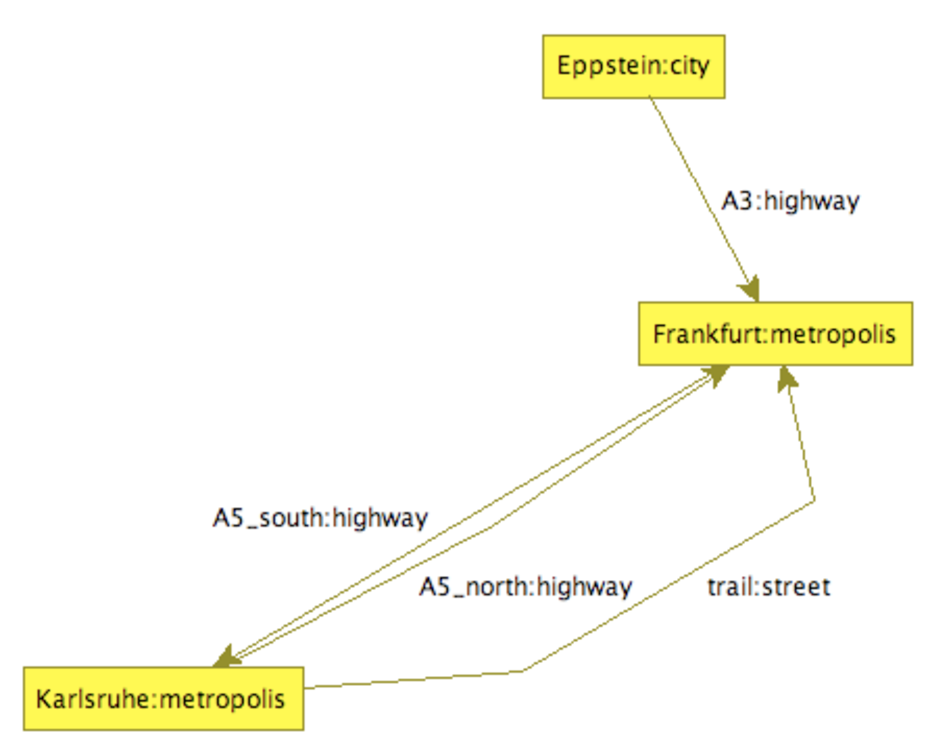
\includegraphics[width=8.5cm]{fig/map}}
\end{center}

This graph is valid but not strict valid.
\begin{grshell} 
> validate
The graph is valid.
> validate strict
The graph is NOT valid:
  CAE: city "Eppstein" -- highway "A3" --> metropolis "Frankfurt" not specified
  CAE: metropolis "Karlsruhe" -- street "trail" --> metropolis "Frankfurt" not specified
>
\end{grshell}
\end{example}


\pagebreak

\subsection{Graph Input and Output Commands}
\label{outputcmds}

\begin{rail}
  'save' 'graph' Filename
\end{rail}\ixkeyw{save}\ixkeyw{graph}
Dumps\indexmain{dumping graph} the current graph as \GrShell\ script\indexmain{graph rewrite script} into \emph{Filename}.
The created script includes
\begin{itemize}
  \item selecting the backend
  \item creating a new graph with all nodes and edges (including their persistent names)
  \item restoring the (graph global) variables
  \item restoring the visualisation styles
\end{itemize}
but not necessarily using the same commands you typed in during construction. 
Such a script can be loaded and executed by the \texttt{include} command (see Section~\ref{commcommands}).

\begin{rail}
  'export' Filename ('.grs' | '.grsi') ('.gz')? ('withvariables')?
\end{rail}\ixkeyw{export}\ixkeyw{withvariables}\indexmain{export}
Exports an instance graph in GRS (.grs/.grsi) format, which is a reduced \GrShell\ script
(it can get imported and exported on API level\ref{sub:imexport} without using the \GrShell).
It contains the \texttt{new graph} command, followed by \texttt{new node} commands, followed by \texttt{new edge} commands.
If the \texttt{.gz} suffix is given the graph is saved zipped.
If \texttt{withvariables} is specified, the (graph global) variables are exported, too.
The export is only complete with the model of the graph given in the \texttt{.gm} file.
Exporting fails if the graph model contains attributes of \texttt{object}-type.
The \texttt{save} command is for saving about a \GrShell\ session including graph global variables and visualization commands, 
the goal of the \texttt{export} command is basic graph rewrite system interoperability.
The persistent names are saved in contrast to the following format GXL.

\begin{rail}
  'export' Filename '.gxl' ('.gz')?
\end{rail}\ixkeyw{export}\indexmain{import}
Exports an instance graph and a graph model in GXL format \cite{GXL,GXL2}, 
which is somewhat of a standard format for graphs of graph rewrite systems, 
but suffers from the well-known XML problems -- it is barely human-readable and bloated.
Exporting fails if the graph model contains attributes of \texttt{set<S>}-,\texttt{map<S,T>}-, or \texttt{object}-type.
If the \texttt{.gz} suffix is given the graph is saved zipped.

\begin{rail}
  'import' Filename ('.grs' | '.grsi' ) ('.gz')?
\end{rail}\ixkeyw{import}
Imports the specified graph instance in GRS (.grs/.grsi) format (the \emph{reduced} \GrShell\ script,
a saved graph can only be imported by \texttt{include} (but an exported graph can be imported by \texttt{include}, too)).
The referenced graph model must be available as \texttt{.gm}-file.
If the \texttt{.gz} suffix is given the graph is expected to be zipped.

\begin{rail}
  'import' Filename '.gxl' ('.gz')? (ModelOverride)?
\end{rail}\ixkeyw{import}
Imports the specified graph instance and model in GXL format.
If a model override of the form \texttt{Filename.gm} is specified, the given model will be used instead of the model in the GXL file.
The \texttt{.gxl}-graph must be compatible to the \texttt{.gm}-model.
If the \texttt{.gz} suffix is given the graph is expected to be zipped.

\begin{note}\label{shellgxlimport}
Normally you are not only interested in importing a GXL graph (and viewing it), but you want to execute actions on it.
The problem is that the actions are model dependent.
So, in order to apply actions, you must use a model override, which works this way:
\begin{enumerate}
\item \texttt{new graph "YourName.grg"}\\
This creates the model library lgsp-YourNameModel.dll
and the actions library lgsp-YourNameActions.dll
(which depends on the model library generated from the \texttt{"using YourName;"}).
\item \texttt{import InstanceGraphOnly.gxl YourName.gm}\\
This imports the instance graph from the .gxl but uses the model specified
in YourName.gm (it must fit to the model in the .gxl in order to work).
\item \texttt{select actions lgsp-YourNameActions.dll}\\
This loads the actions from the actions library in addition to the already
loaded model and instance graph (cf. \ref{grsthings}).
\item Now you are ready to use the actions.
\end{enumerate}
\end{note}

\begin{note}\label{shellecoreexport}
Further formats available for import are \texttt{.ecore} plus \texttt{.xmi}.
These are formats common to the model transformation community which are not directly geared towards graphs, so they can't be imported directly.
Instead during the import process an intermediate \texttt{.gm} is written which is equivalent to the \texttt{.ecore} given -- you may inspect it to see how the content gets mapped
(the importer maps classes to GrGen node classes, their attributes
to corresponding GrGen attributes, and their references to GrGen
edge classes; inheritance is transferred one-to-one, and enumerations are
mapped to GrGen enums; class names are prefixed by the names of the
packages they are contained in to prevent name clashes).
After this metamodel transformation the instance graph XMI adhering to the Ecore model thus adhering to the just
generated equivalent GrGen graph model gets imported.
Furthermore you can give specify a \texttt{.grg} containing the rules to apply (using further rule and model files).
The importer was added for a GraBaTs challenge and is available as-is -- it may or may not work for you, 
if you need more it's on you to improve it. An export is not available -- we coded the export we needed with emit statements.
\begin{rail}
  'import' ((Filename '.ecore')+( )) Filename '.xmi' (Filename '.grg')?
\end{rail}\ixkeyw{import}
\end{note}

\begin{rail}
  'import' 'add' FileSpec 'withvariables'
\end{rail}\ixkeyw{import}\ixkeyw{add}
Imports the graph in the specified file and adds it to the current graph
(instead of overwriting the old graph with the new graph).
The \texttt{FileSpec} is of the same format as the file specification in the other two imports.
The \texttt{withvariables} argument only yields an effect if the file to import contains variable specifications (the content of old variables of the same name is overwritten).


\subsection{Graph Manipulation Commands}
\label{mani}
Graph manipulation commands alter existing graphs; they allow to create and delete graph elements and change attributes. 
These are tasks which should be carried by the rules of the rule language -- the commands are mainly used as elementary instructions in graph input and output.

\begin{rail}
  'new' (() | Text) (() | ':' NodeType (() | Constructor))
\end{rail}\ixkeyw{new}
Creates a new node within the current graph.
Optionally a variable \emph{Text} is assigned to the new node.
If \emph{NodeType} is supplied, the new node will be of type \emph{NodeType} and attributes can be initialized by a constructor.
Otherwise the node will be of the base node class type \emph{Node}.
\begin{note}
The \GrShell\ can reassign \indexed{variable}s. 
This is in contrast to the rule language (Chapter~\ref{chaprulelang}), where we use \emph{names}\indexmain{name}\indexmain{expression variable}\indexmainsee{expression variable}{name}.
\end{note}

\begin{rail}
  'new' Node (('-' EdgeEntityConstructor '->') | ('-' EdgeEntityConstructor '-')) Node ;
EdgeEntityConstructor:
  (()|Text) (() | ':' EdgeType (() | Constructor)) ;
\end{rail}\ixkeyw{new}
Creates a new edge within the current graph between the specified nodes,
directed from the first to the second \emph{Node} in the case of \texttt{-->},
or undirected in the case of \texttt{--}.
Optionally a variable \emph{Text} is assigned to the new edge.
If \emph{EdgeType} is supplied, the new edge will be of type \emph{EdgeType} and attributes can be initialized by a constructor.
Otherwise the edge will be of the base edge class type \texttt{Edge} for \texttt{-->} or \texttt{UEdge} for \texttt{--}.

\begin{rail}
  Constructor : '(' (() | (dollar '=' Text (() | ',' Attributes) | Attributes)) ')';
  Attributes : (AttributeName '=' AttributeValue) + (',');
  AttributeValue :  PrimitiveAttributeValue | SetConstr | MapConstr ;
  PrimitiveAttributeValue : EnumLit | Number | DoubleNum | FloatNum | QuotedText | BoolLit | NullLit ;
  SetConstr: 'set' '<' Type '>' lbrace ( Expression*',' ) rbrace ;
  MapConstr: 'map' '<' Type ',' Type '>' \\ lbrace ( (Expression '->' Expression)*',' ) rbrace ;
\end{rail}\indexmain{\texttt{\$}}\ixnterm{Constructor}\ixnterm{Attributes}\ixnterm{AttributeValue}\ixnterm{PrimitiveAttributeValue}\ixnterm{SetConstr}\ixnterm{MapConst}
A \indexed{constructor} is used to initialize a new graph element (see \texttt{new \dots} below).
A comma separated list of \indexed{attribute} declarations is supplied to the constructor.
Available attribute names are specified by the graph model of the current working graph.
All the undeclared attributes will be initialized with \indexed{default value}s, depending on their type 
(\texttt{int} $\leftarrow$ \texttt{0}; \texttt{boolean} $\leftarrow$ \texttt{false}; \texttt{float} $\leftarrow$ \texttt{0.0f}; \texttt{double} $\leftarrow$ \texttt{0.0}; \texttt{string} $\leftarrow$ \texttt{""}; \texttt{set<T>} $\leftarrow$ \texttt{set<T>\{\}}; \texttt{map<S,T>} $\leftarrow$ \texttt{map<S,T>\{\}}; \texttt{enum} $\leftarrow$ unspecified;).\\
The \texttt{\$} is a special attribute name: a unique identifier of the new graph element.
This identifier is also called \newterm{persistent name} (see Example~\ref{persistentex}).
This name can be specified by a constructor only.

\begin{rail}
  'delete' 'node' Node
\end{rail}\ixkeyw{delete}\ixkeyw{node}
Deletes the node \emph{Node} from the current graph.
Incident edges will be deleted as well.

\begin{rail}
  'delete' 'edge' Edge
\end{rail}\ixkeyw{delete}\ixkeyw{edge}
Deletes the edge \emph{Edge} from the current graph.

\begin{rail}
  GraphElement '.' AttributeName '=' (Text | Number) ;
\end{rail}
Set the \indexed{attribute} \emph{AttributeName} of the graph element \emph{GraphElement} to the value of \emph{Text} or \emph{Number}.

  
\subsection{Graph and Model Query Commands}

\begin{rail}
  'show' (() | 'num') ('nodes' (() | (() | 'only') NodeType) | 'edges' (() | (() | 'only') EdgeType))
\end{rail}\ixkeyw{show}\ixkeyw{num}\ixkeyw{nodes}\ixkeyw{edges}\ixkeyw{only}
Gets the \indexed{persistent name}s and the types of all the nodes/edges of the current graph. 
If a node type or edge type is supplied, only elements compatible to this type are considered. 
The \texttt{only} keyword excludes subtypes. Nodes/edges without persistent names are shown with a pseudo-name.
If the command is specified with \texttt{num}, only the number of nodes/edges will be displayed.

\begin{rail}
  'show' ('node' | 'edge') 'types'
\end{rail}\ixkeyw{show}\ixkeyw{node}\ixkeyw{edge}\ixkeyw{types}
Gets the node/edge types of the current graph model.

\begin{rail}
'show' ('node' ('super' | 'sub') 'types' NodeType | 'edge' ('super' | 'sub') 'types' EdgeType)
\end{rail}\ixkeyw{show}\ixkeyw{node}\ixkeyw{edge}\ixkeyw{super}\ixkeyw{sub}\ixkeyw{types}\indexmain{inheritance}
Gets the inherited/descendant types of \emph{NodeType}/\emph{EdgeType}.

\begin{rail}
  'show' ('node' 'attributes' (() | (() | 'only') NodeType) | 'edge' 'attributes' (() | (() | 'only') EdgeType))
\end{rail}\ixkeyw{show}\ixkeyw{node}\ixkeyw{edge}\ixkeyw{only}\ixkeyw{attributes}
Gets the available node/edge \indexed{attribute} types.
If \emph{NodeType}/\emph{EdgeType} is supplied, only attributes defined in \emph{NodeType}/\emph{EdgeType} are diplayed.
The \texttt{only} keyword excludes inherited attributes.\\
\begin{note}
The \texttt{show nodes/edges attributes\dots} command covers types and \emph{inherited} types.
This is in contrast to the other \texttt{show\dots} commands where types and \emph{sub}types are specified or the direction in the type hierarchy is specified explicitly, respectively.
\end{note}

\begin{rail}
 'show' ('node' Node | 'edge' Edge)
\end{rail}\ixkeyw{show}\ixkeyw{node}\ixkeyw{edge}
Gets the attribute types and values of a specific graph element.

\begin{rail}
  'show' GraphElement '.' AttributeName
\end{rail}\ixkeyw{show}
Displays the value of the specified attribute.

\begin{rail}
  'node' 'type' Node 'is' Node | 'edge' 'type' Edge 'is' Edge
\end{rail}\ixkeyw{node}\ixkeyw{edge}\ixkeyw{type}\ixkeyw{is}
Gets the information whether the first element is \indexed{type-compatible}\indexmainsee{compatible types}{type-compatible} to the second element.


\subsection{Graph Visualization Commands}\label{sub:visual}\indexmain{visualization}\indexmainsee{layout}{visualization}\indexmainsee{visualization}{group node}

\begin{rail}
  'show' 'graph' ExecutableName (() | Text)
\end{rail}\ixkeyw{show}\ixkeyw{graph}
Dumps the current graph in \indexed{VCG} format into a temporary file.
The temporary VCG file will be passed to the program \emph{ExecutableName} as first parameter;
further parameters, such as program options, can be specified by \emph{Text}.
If you use \yComp\footnote{See Section~\ref{tools:ycomp}.}\indexmain{yComp} as executable (\texttt{show graph ycomp}), this may look like
\begin{center}
  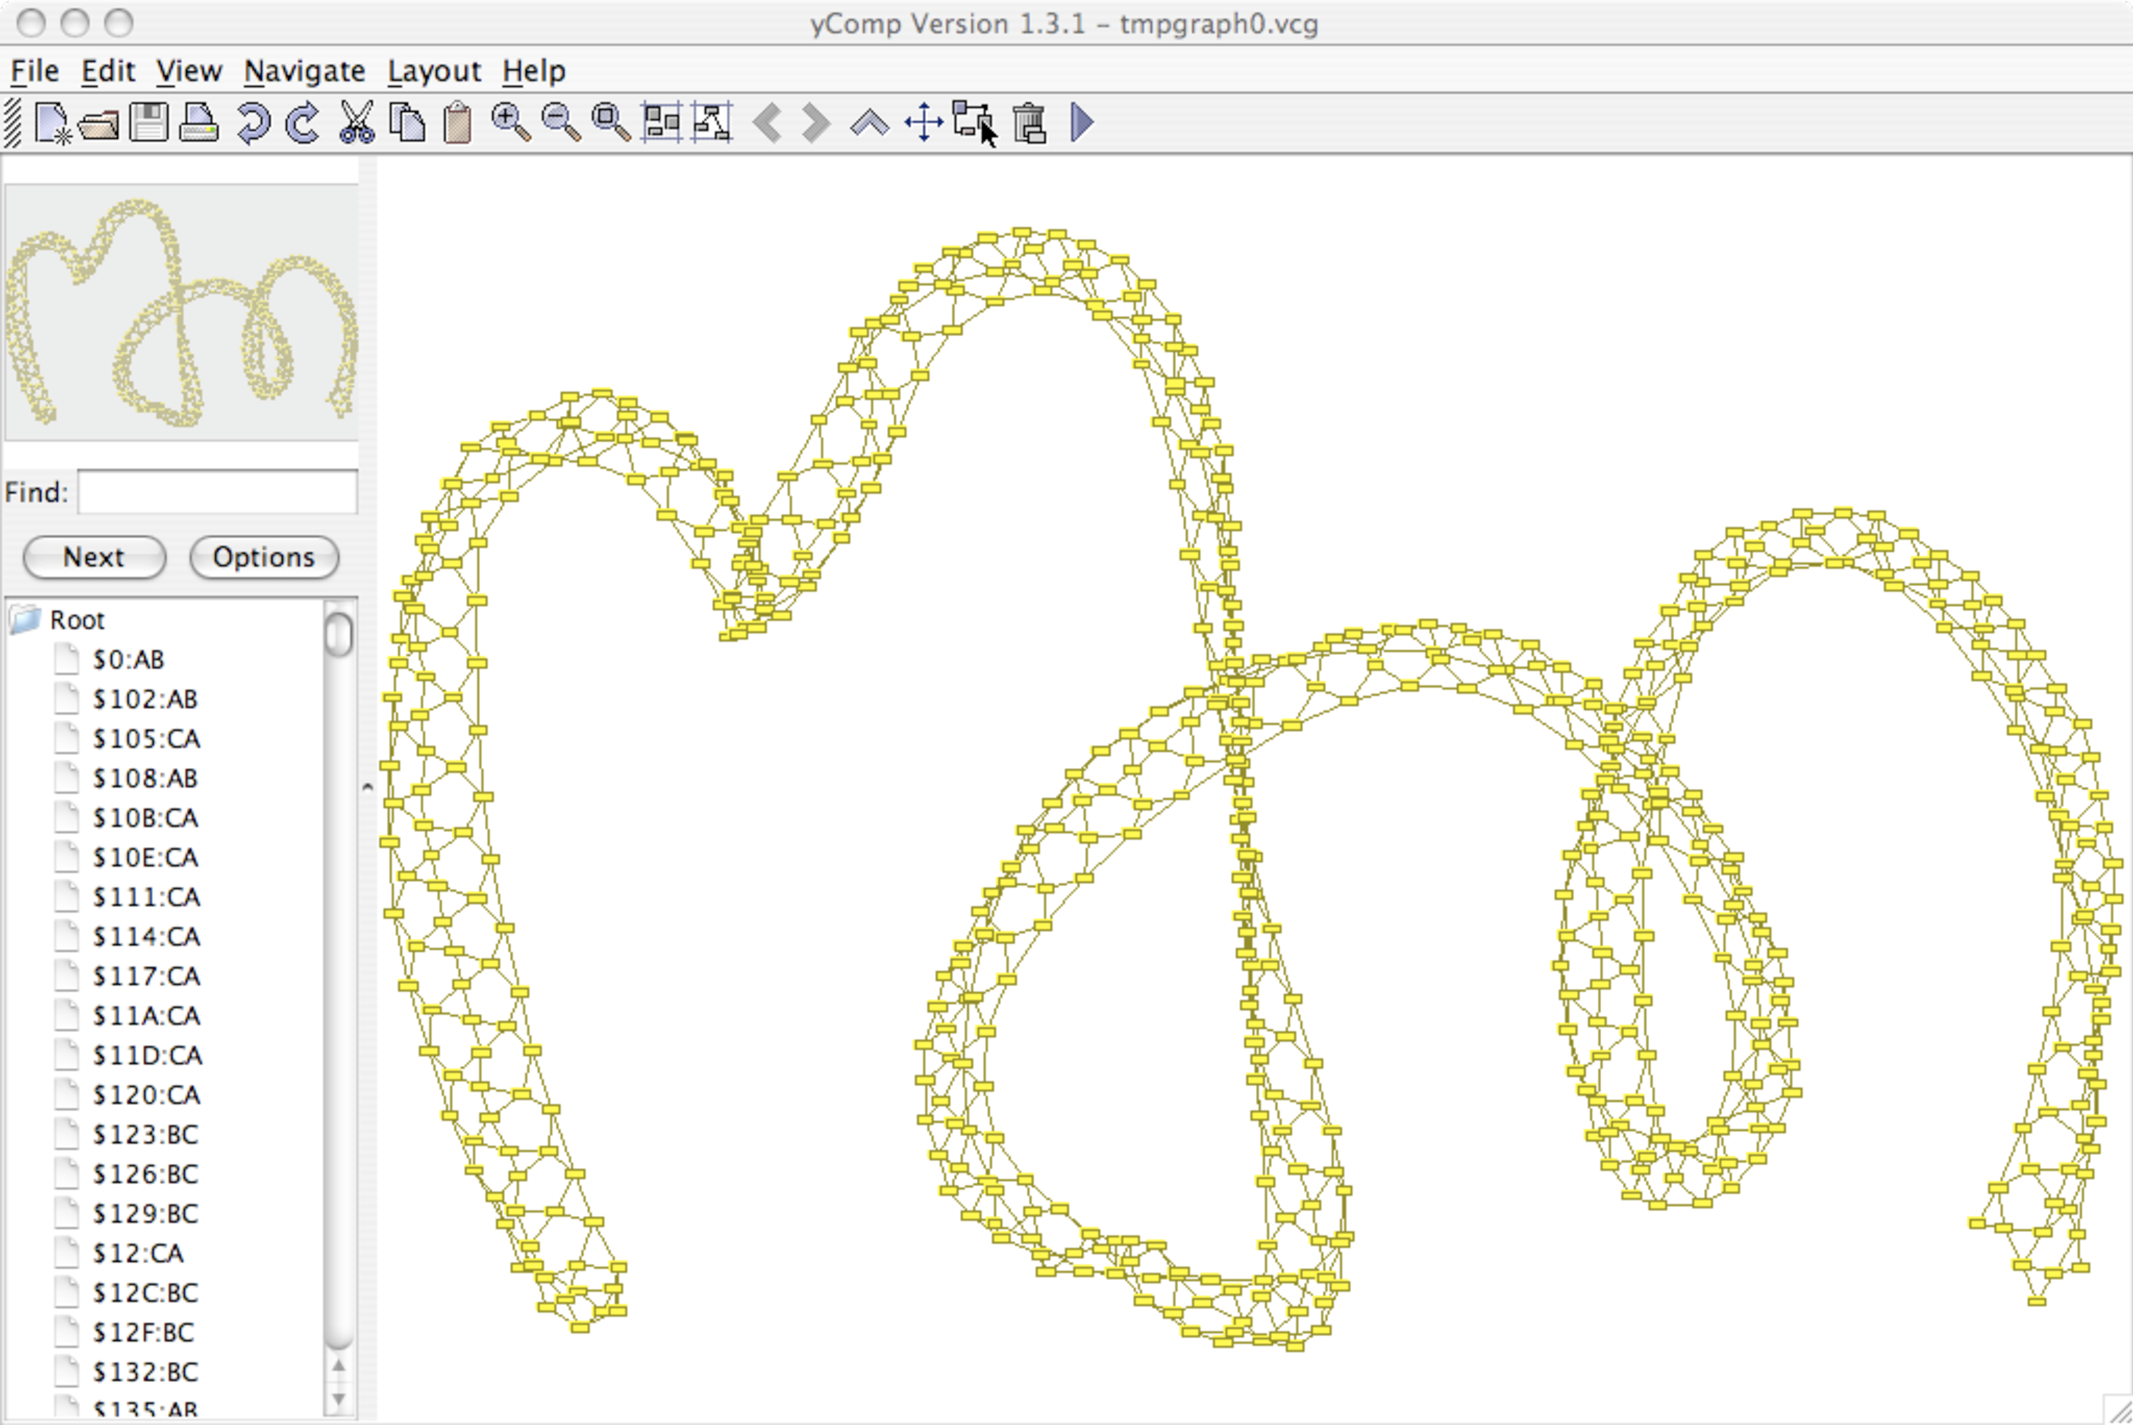
\includegraphics[width=0.75\linewidth]{fig/showgraph}
\end{center}  
The temporary file will be deleted, when the application \emph{Filename} is terminated if \GrShell\ is still running at this time.

\begin{rail}
  'dump' 'graph' Filename
\end{rail}\ixkeyw{dump}\ixkeyw{graph}
Dumps the current graph in \indexed{VCG} format into the file \emph{Filename}.\\

The following commands control the style of the VCG output. This affects \texttt{dump graph}, \texttt{show graph}, and \texttt{enable debug}. 
\begin{rail}
  'dump' 'set' 'node' (() | 'only') NodeType \\ (('color' | 'textcolor' | 'bordercolor') Color | 'shape' Text | 'labels' ('on' | 'off' | Text)) ;
\end{rail}\ixkeyw{dump}\ixkeyw{set}\ixkeyw{node}\ixkeyw{only}\ixkeyw{color}\ixkeyw{textcolor}\ixkeyw{bordercolor}\ixkeyw{shape}\ixkeyw{labels}\ixkeyw{on}\ixkeyw{off}
Sets the \indexed{color}, text color, border color, the shape or the label of the nodes of type \emph{NodeType} and all of its subtypes.
The keyword \texttt{only} excludes the subtypes. The available colors are specified at the begin of this chapter. 
The following shapes are supported: \texttt{box}, \texttt{triangle}, \texttt{circle}, \texttt{ellipse}, \texttt{rhomb}, \texttt{hexagon}, \texttt{trapeze}, \texttt{uptrapeze}, \texttt{lparallelogram}, \texttt{rparallelogram}.
Those are shape names of \yComp\ (for a VCG definition see~\cite{vcg}).
The default labeling is set to \texttt{on} with \texttt{Name:Type}, it can be overwritten by an specified label string (e.g. the source code line originating the node in a program graph) or switched off.

\begin{rail}
  'dump' 'set' 'edge' (() | 'only') EdgeType \\ (('color' | 'textcolor') Color | 'labels' ('on' | 'off' | Text));
\end{rail}\ixkeyw{dump}\ixkeyw{set}\ixkeyw{edge}\ixkeyw{only}\ixkeyw{color}\ixkeyw{textcolor}\ixkeyw{labels}\ixkeyw{on}\ixkeyw{off}
Sets the color, text color or label of the edges of type \emph{EdgeType} and all of its subtypes.
The keyword \texttt{only} excludes the subtypes. The available colors are specified at the begin of this chapter.
The default labeling is set to \texttt{on} with \texttt{Name:Type}, it can be overwritten by an specified label string or switched off.

\begin{rail}
  'dump' 'add' (('node' ('only')? NodeType)|('edge' ('only')? EdgeType)) 'exclude' ;
\end{rail}\ixkeyw{dump}\ixkeyw{add}\ixkeyw{node}\ixkeyw{edge}\ixkeyw{only}\ixkeyw{exclude}
Excludes nodes/edges of type \emph{NodeType}/\emph{EdgeType} and all of its subtypes from output, for a node it also excludes its incident edges.
The keyword \texttt{only} excludes the subtypes from exlusion, i.e.\ subtypes of \emph{NodeType}/\emph{EdgeType} are dumped.

\begin{rail}
  'dump' 'add' 'node' ('only')? NodeType 'group' (GroupConstraints)? ;
GroupConstraints:
  'by' ('hidden')? GroupMode (IncAdjTypeConstraints)? ;
IncAdjTypeConstraints:
  ('only')? EdgeType ('with' ('only')? NodeType)? ;
\end{rail}\ixkeyw{dump}\ixkeyw{add}\ixkeyw{node}\ixkeyw{only}\ixkeyw{group}\ixkeyw{by}\ixkeyw{hidden}\ixkeyw{with}\ixnterm{GroupConstraints}\ixnterm{IncAdjTypeConstraints}
Declares \emph{NodeType} and subtypes of \emph{NodeType} as \indexed{group node}\indexmainsee{hierarchic}{group node} type.
All the differently typed nodes that point to a node of type \emph{NodeType} 
(i.e.\ there is a directed edge between such nodes) will be grouped and visibly enclosed by the \emph{NodeType}-node.
\texttt{GroupMode} is one of \texttt{no},\texttt{incoming},\texttt{outgoing},\texttt{any}; \texttt{hidden} causes hiding of the edges by which grouping happens.
The \texttt{EdgeType} constrains the type of the edges which cause grouping, the \texttt{with} clause additionally constrains the type of the adjacent node; 
\texttt{only} excludes subtypes.

\begin{note}
Only apply group commands on a graph if they indeed lead to a containment tree of groups.
If the group commands would lead to a directed acyclic or even cyclic containment graph, the results are undefined.
You may get duplicate edges (and nodes); the implementation is free to choose indeterministically between the possible nestings -- it may even grow an arm and stab you in your back.
(A conflict resultion heuristic used is to give the earlier executed \texttt{add group} command priority. 
But this mechanism is incomplete -- you'd better refine your groups or change the model in that case.
Using a model separating edges denoting direct containment from cross-linking edges by type is normally the better design, even disregarding visual node nesting.)
\end{note}

The following example shows \emph{metropolis} ungrouped and grouped:
\begin{center}
  \fbox{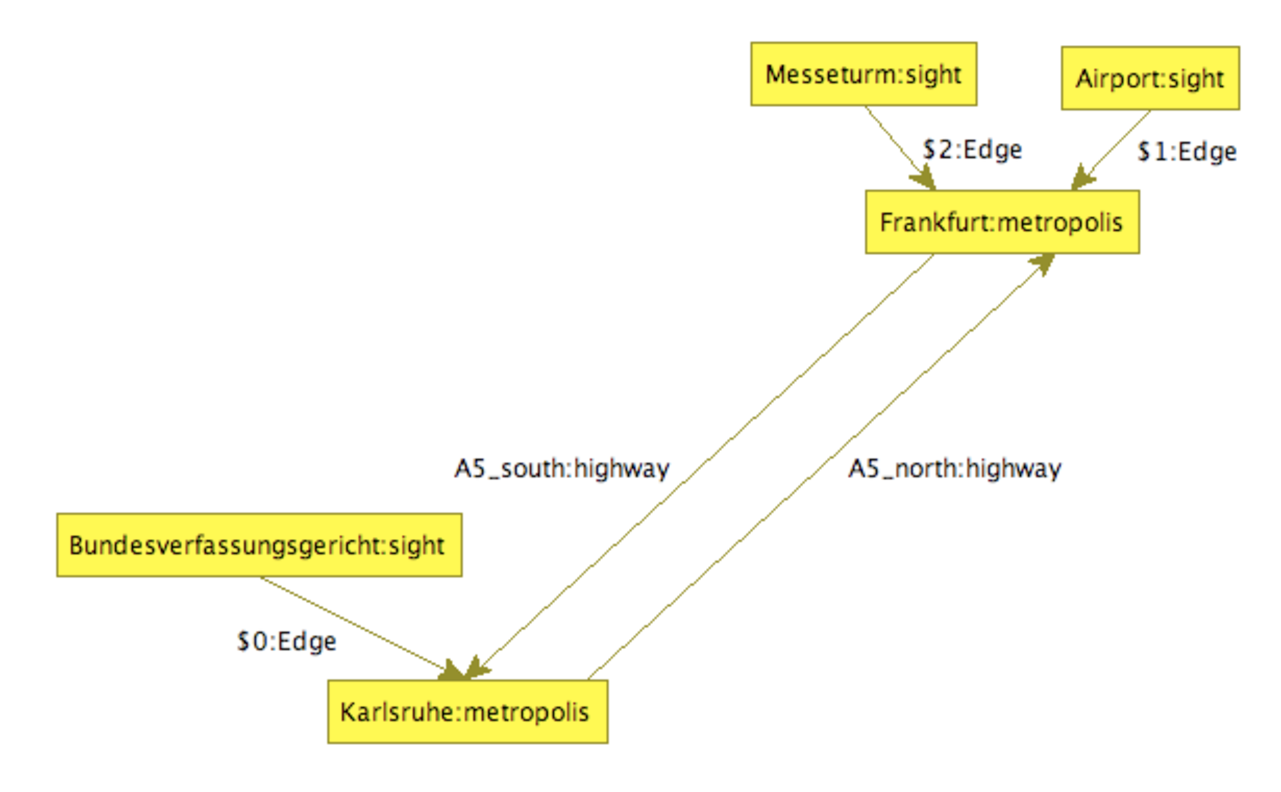
\includegraphics[width=0.45\linewidth]{fig/group2-1}}  \hfill \fbox{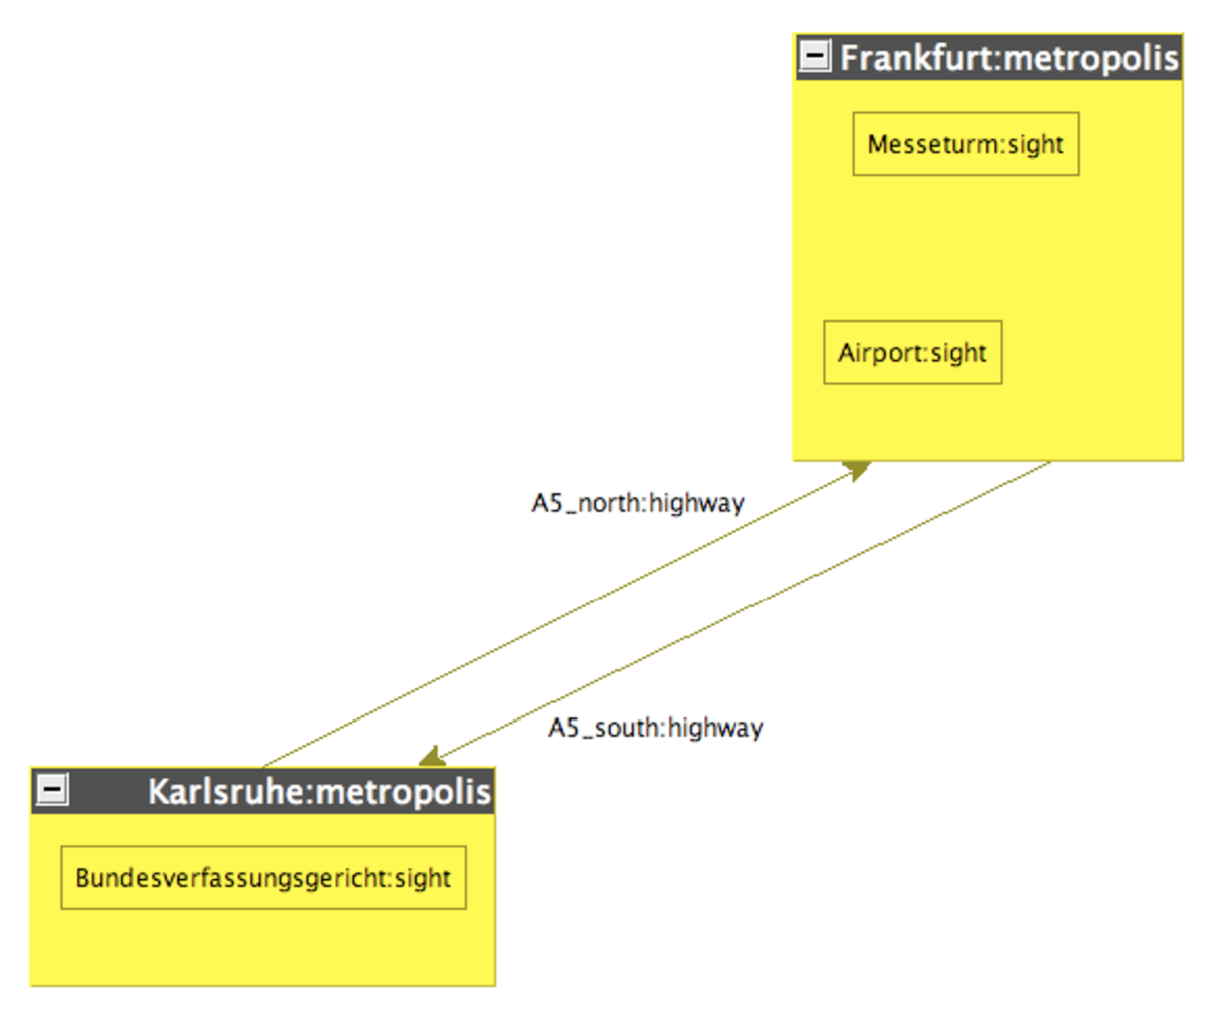
\includegraphics[width=0.45\linewidth]{fig/group2-2}}\\
  {\small right side: dumped with \texttt{dump add node metropolis group}}
\end{center}

\begin{rail}
  'dump' 'add' (() | 'only') ('node' NodeType | 'edge' EdgeType) \\ ('infotag' | 'shortinfotag') AttributeName
\end{rail}\ixkeyw{dump}\ixkeyw{add}\ixkeyw{only}\ixkeyw{node}\ixkeyw{edge}\ixkeyw{infotag}\ixkeyw{shortinfotag}
Declares the \indexed{attribute} \emph{AttributeName} to be an ``\indexed{info tag}'' or ``\indexed{short info tag}''.
Info tags are displayed like additional node/edge \indexed{label}s, in format \texttt{Name=Value}, or \texttt{Value} only for short info tags. 
The keyword \texttt{only} excludes the subtypes of \emph{NodeType} resp.\ \emph{EdgeType}. 
In the following example \emph{river} and \emph{jam} are info tags:
\begin{center}
  \fbox{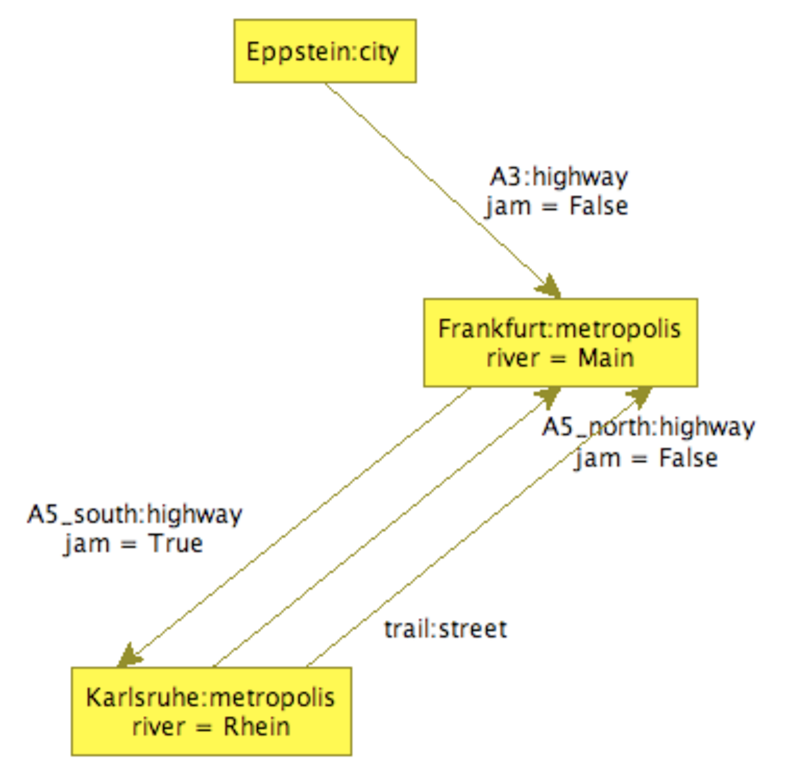
\includegraphics[width=0.5\linewidth]{fig/infotag}}
\end{center}

\begin{rail}
  'dump' 'reset'
\end{rail}\ixkeyw{dump}\ixkeyw{reset}
Resets all style options (\texttt{dump set}\dots) and (\texttt{dump add}\dots) to their default values.


\begin{note}\label{note:visual}
Small graphs allow for fast visual understanding, but with an increasing number of nodes and edges they quickly loose this property.
The group commands are of outstanding importance to keep readability with increasing graph sizes
(e.g. for program graphs it allows to lump together expressions of a method inside the method node and attributes of the class inside the class node).
Additional helpers in keeping the graph readable are: 
the capability to exclude elements from dumping (the less hay in the stack the easier to find the needle),
the different colors and shapes to quickly find the elements of interest,
as well as the labels/infotags/shortinfotags to display the most important information directly. 
Choose the layout algorithm and the options delivering the best results for your needs, organic and hierarchic or compiler graph 
(an extension of hierarchic with automatic edge cutting -- marking cut edges by fat dots, showing the edge only on mouse over and allowing to jump to the other end on a mouse click)
should be tried first.
\end{note}

The following example shows several of the layout options employed to considerably increase the readability of a program graph (as given in \texttt{examples/JavaProgramGraphs-GraBaTs08}):
\begin{center}
  \fbox{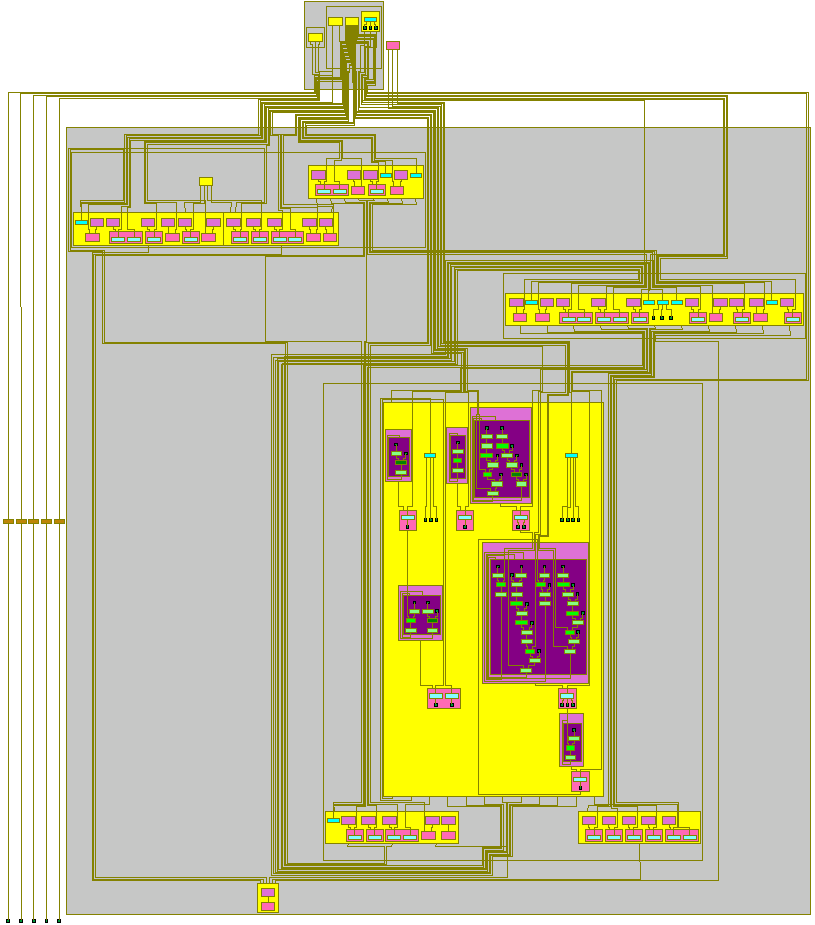
\includegraphics[width=0.45\linewidth]{fig/screen-overview}}  \hfill \fbox{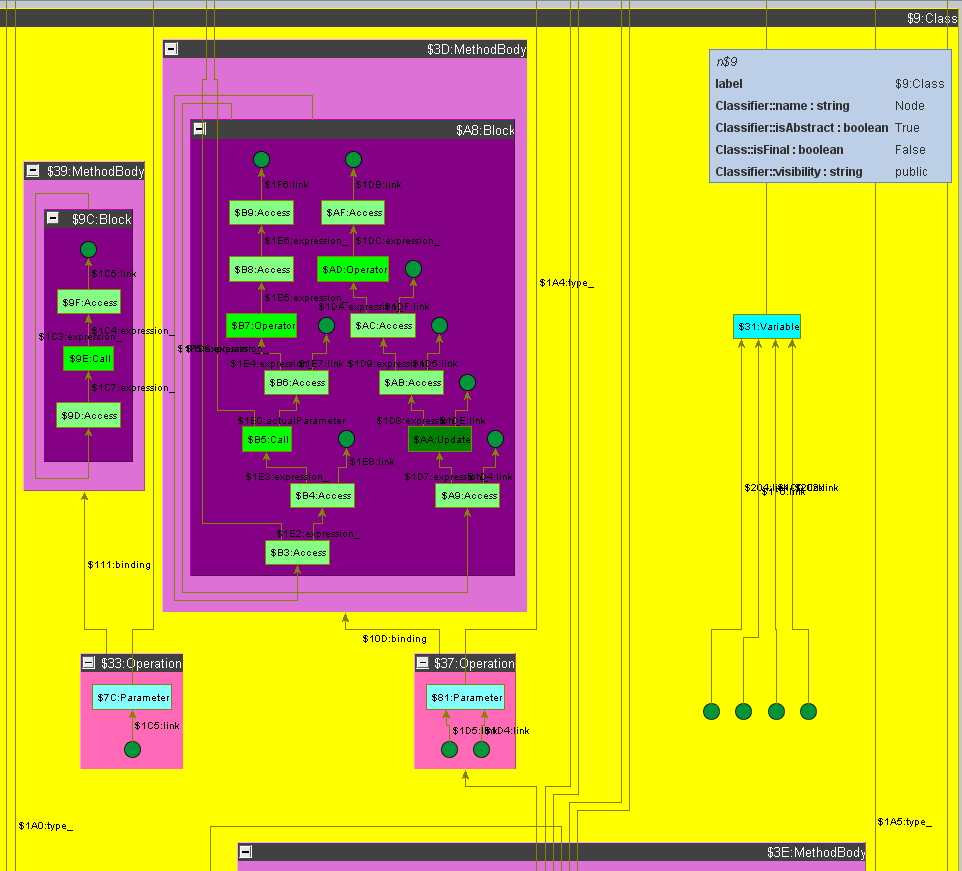
\includegraphics[width=0.45\linewidth]{fig/screen-detail}}\\
  {\small Overview of the initial program graph and some details of the ``Node'' class}
\end{center}


\subsection{Action Commands (XGRS)}\indexmain{action command}\indexmainsee{action}{graph rewrite sequence}
\label{grsthings}
An \emph{action} denotes a graph rewrite rule.

\begin{rail}
  'select' 'actions' Filename
\end{rail}\ixkeyw{select}\ixkeyw{actions}
Selects a \indexed{rule set}.
\emph{Filename} can either be a .NET assembly (e.g.\ ``rules.dll'') or a source file (``rules.cs'').
Only one rule set can be loaded simultaneously.

\begin{rail}
  'show' 'actions'
\end{rail}\ixkeyw{show}\ixkeyw{actions}
Lists all the rules of the loaded rule set, their parameters, and their return values.
Rules can return a set of graph elements.

\begin{rail}
  'custom' 'actions' (() | SpacedParameters)
\end{rail}\ixkeyw{custom}\ixkeyw{actions}
Executes an action specific to the current \indexed{backend}. 
If \emph{SpacedParameters} is omitted, a list of available commands will be displayed (for the LGSPBackend see Section~\ref{custom}).

\makeatletter
\begin{rail}
  GraphRewriteSequence: 'xgrs' SimpleRewriteSequence ;
\end{rail}\ixkeyw{xgrs}\indexmain{graph rewrite sequence}\indexmainsee{GRS}{graph rewrite sequence}\ixnterm{GraphRewriteSequence}
This executes the graph rewrite sequence \emph{SimpleRewriteSequence}.
See Chapter~\ref{cha:xgrs} for graph rewrite sequences.
Additionally to the variable assignment in rule-embedded graph rewrite sequences, you are also able to assign \emph{persistent names} to parameters via  \texttt{Variable = \@(Text)}.

Graph elements returned by rules can be assigned to variables\indexmain{variable} using \texttt{(Para\-meters) = \emph{Action}}\indexmain{parameter}. 
The desired variable identifiers have to be listed in \emph{Parameters}. 
Graph elements required by rules must be provided using \texttt{Action (Para\-meters)}, where \emph{Parameters} is a list of variable identifiers. 
For \indexed{undefined variables} see Section~\ref{ruledecls}, \emph{Parameters}.

% don't explain set/map commands, as they will be replaced by graph rewrite sequence terms
% they are given in the changelog, so if someone needs them now they are there
% but not fully officially documented, so that they can be dropped as soon as the sequences are extended


\section{Graphical Debugger}
\label{sct:debugger}
The \GrShell\ together with \yComp\ build \GrG's graphical debugger.

\subsection{Debugging Related Commands}

\begin{rail}
  'debug' ( 'enable' | 'disable' )
\end{rail}\ixkeyw{debug}\ixkeyw{enable}\ixkeyw{disable}
Enables and disables the \indexed{debug mode}.
The debug mode shows the current working graph in a \yComp\ window.
All changes to the working graph are tracked by \yComp\ immediately.  

\begin{rail}
  'debug' 'set' 'layout' ( (Text)? | 'option' Name String ) ;
\end{rail}\ixkeyw{debug}\ixkeyw{set}\ixkeyw{layout}\ixkeyw{option}
Sets the default graph \indexed{layout algorithm} to \emph{Text}.
If \emph{Text} is omitted, a list of available layout algorithms is displayed.
See Section~\ref{tools:ycomp} on \yComp\ layouters.
The \texttt{option} version allows to specify layout options by name value pairs.
The available layout options can be listed by the following command.

\begin{rail}
  'debug' 'get' 'layout' 'options';
\end{rail}\ixkeyw{debug}\ixkeyw{get}\ixkeyw{layout}\ixkeyw{options}
Prints a list of the available layout options of the layout algorithm.

\begin{rail}
  'debug' 'layout';
\end{rail}\ixkeyw{debug}\ixkeyw{layout}
Forces re-layout of the graph shown in yComp (same as pressing the play button within yComp).

\begin{rail}
  GraphRewriteSequence: 'debug' 'xgrs' SimpleRewriteSequence ;
\end{rail}\ixkeyw{debug}\ixkeyw{xgrs}\indexmain{graph rewrite sequence}\indexmainsee{GRS}{graph rewrite sequence}\ixnterm{GraphRewriteSequence}
This executes the graph rewrite sequence \emph{SimpleRewriteSequence} in the debugger\indexmain{debugger}.
Same as \texttt{xgrs SimpleRewriteSequence} in the previous section, but allows tracing the rewriting process step-by-step. 


\subsection{Using the Debugger}

The debugging process follows of a series of debug situations,
which result from a user selection of the underlying execution situations along the steps of interest.
During each debugging step the debugger\indexmain{debugger} -- which is a part of the \GrShell~-- 
prints the debugged sequence with the currently focused/active rule highlighted yellow.
What will be shown from executing this rule depends on the commands chosen by the user;
and on the fact whether the focused rule matches or not.
An active rule which is already known to match is highlighted green.
The rule which matched lastly is shown on dark green background,
the rule which failed lastly is shown on dark red background.
During execution \yComp\footnote{Make sure, that the path to your \texttt{\indexed{yComp.jar}} package is set correctly in the \texttt{ycomp} shell script within \GrG's \texttt{/bin} directory.}\indexmain{yComp}
will display the changes to the graph from every single step. 
Besides deciding on what is shown from the execution of the current rule, 
the user determines with the debug commands where to continue the execution
(the rule focused next; but again this depends on success/failure of the currently active rule).
Remember that the \texttt{\%} modifier before a rule works as a break point in a graph rewrite sequence, halting execution and focusing the rule once it is reached.
The debug commands are given in Table~\ref{tabdebug}.
A run is shown in the following example \ref{ex:debug}.
\begin{table}[htbp]
  \begin{tabularx}{\linewidth}{|lX|} \hline
  \texttt{s}(tep) & Execute the current rewrite rule (match, and rewrite in case it matched; the resulting graph is shown).\\
  \texttt{d}(etailed step) & Execute the current rewrite rule in a three-step procedure: matching - highlighting the found match, rewriting - highlighting the changing elements, and doing the rewrite showing the resulting graph. In addtion, afterwards the execution of subrules from embedded xgrs (\texttt{exec}) is shown step by step. \\
  (step) \texttt{o}(ut) & Continue execution until the end of the current loop. If the execution is not in a loop at this moment, the complete sequence will be executed.\\
  (step) \texttt{u}(p) & Ascend one level up within the \indexed{Kantorowitsch tree} of the current rewrite sequence (i.e. rule; see Example~\ref{ex:debug}).\\
  \texttt{n}(ext) & Go to the next rewrite rule which matches, make it current.\\
  (toggle) \texttt{b}(reakpoint) & Toggle a breakpoint at a rewrite rule, or a variable predicate, or a true or false.\\
  \texttt{r}(un) & Continue execution (until the end or a breakpoint).\\
  \texttt{a}(bort) & Cancel the execution immediately.\\ \hline 
  \end{tabularx}
  \caption{\GrShell\ debug commands}
  \label{tabdebug}
\end{table}
%\begin{figure}[htbp]
%  \centering
%  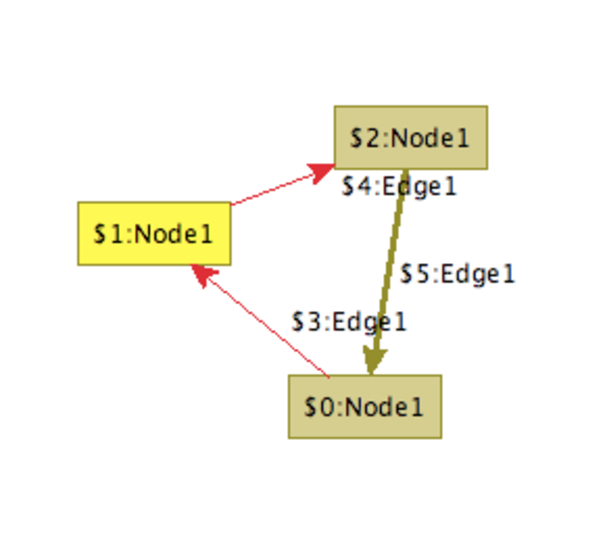
\includegraphics[width=0.25\linewidth]{fig/debug1}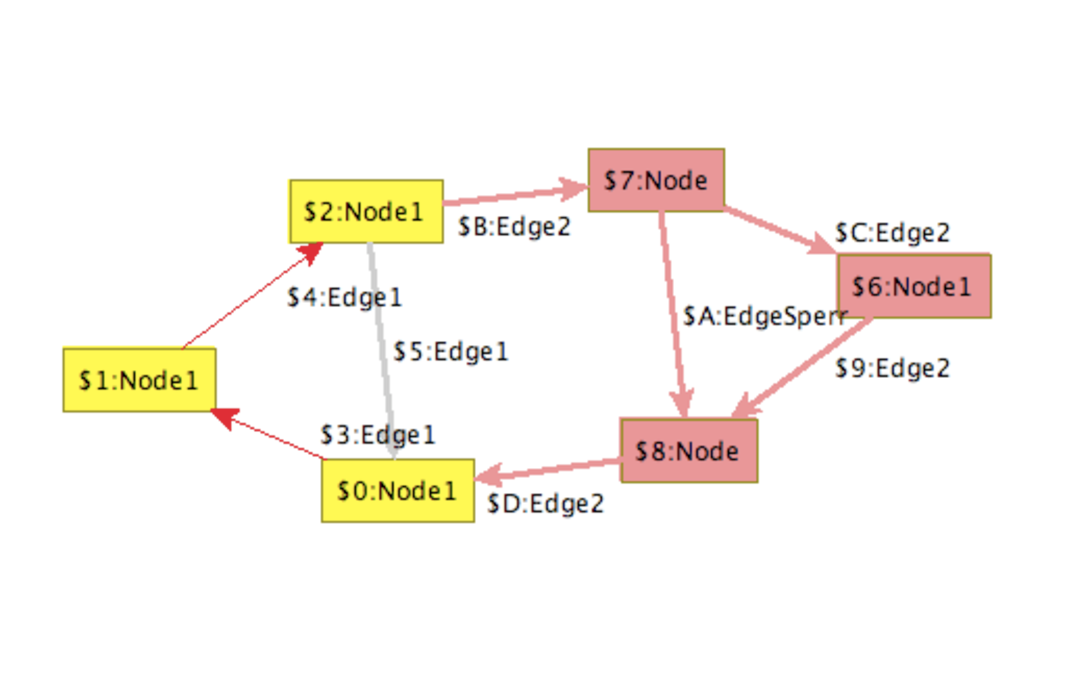
\includegraphics[width=0.4\linewidth]{fig/debug2}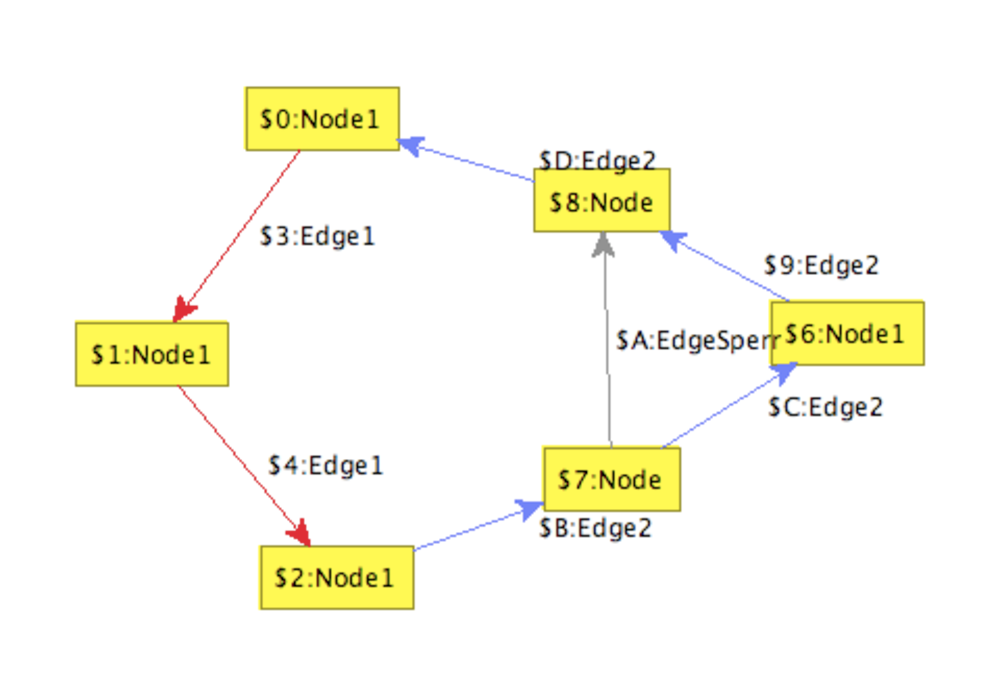
\includegraphics[width=0.4\linewidth]{fig/debug3}
%  \caption{Delayed step rule application.}
%  \label{figdebug}
%\end{figure}

\begin{figure}[htbp]
\begin{example}\label{ex:debug}  
We demonstrate the debug commands with a slightly adjusted script for the Koch snowflake from \GrG's examples (see also Section~\ref{fractals}). The graph rewriting sequence is
\begin{grshell}
debug xgrs (makeFlake1* & (beautify & doNothing)* & makeFlake2* & beautify*)[1]
\end{grshell}
\yComp\ will be opened with an initial graph (resulting from \texttt{grs init}):
\begin{center}
  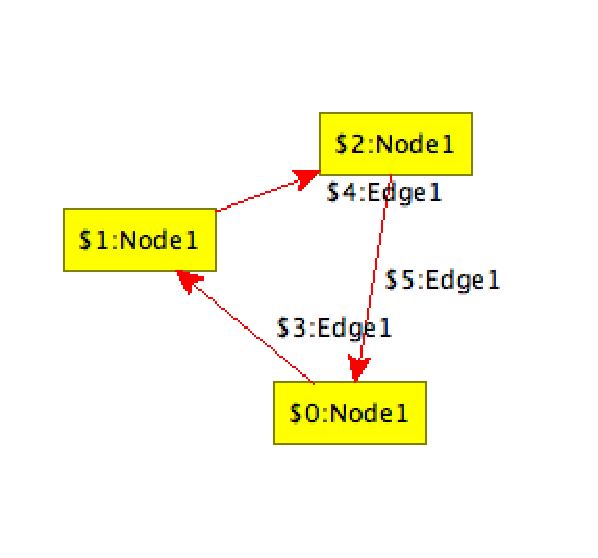
\includegraphics[width=0.3\linewidth]{fig/debug0tra}
\end{center}
We type \texttt{d}(etailed step) to apply \texttt{makeFlake1} step by step resulting in the following graphs:
\begin{center}
  \parbox{0.2\linewidth}{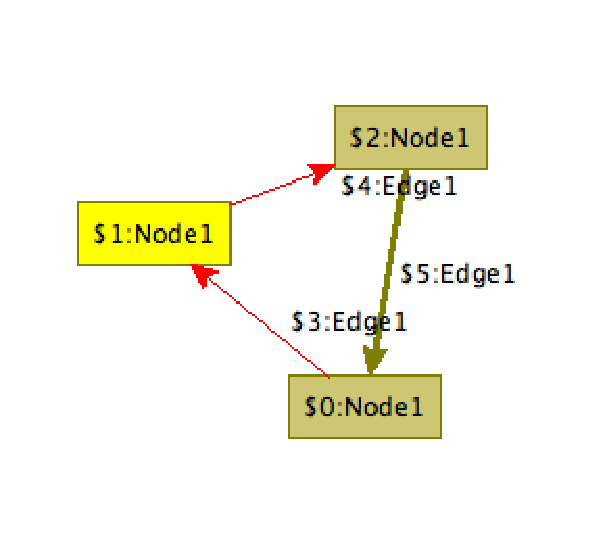
\includegraphics[width=\linewidth]{fig/debug1tra}}\parbox{0.375\linewidth}{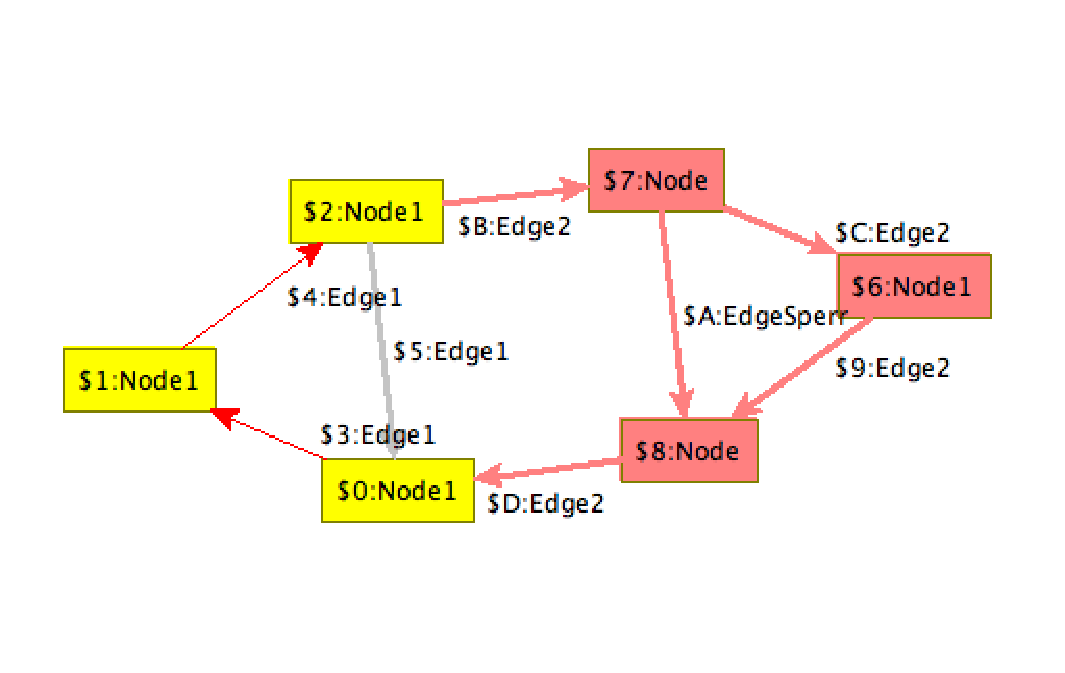
\includegraphics[width=\linewidth]{fig/debug2tra}}\parbox{0.375\linewidth}{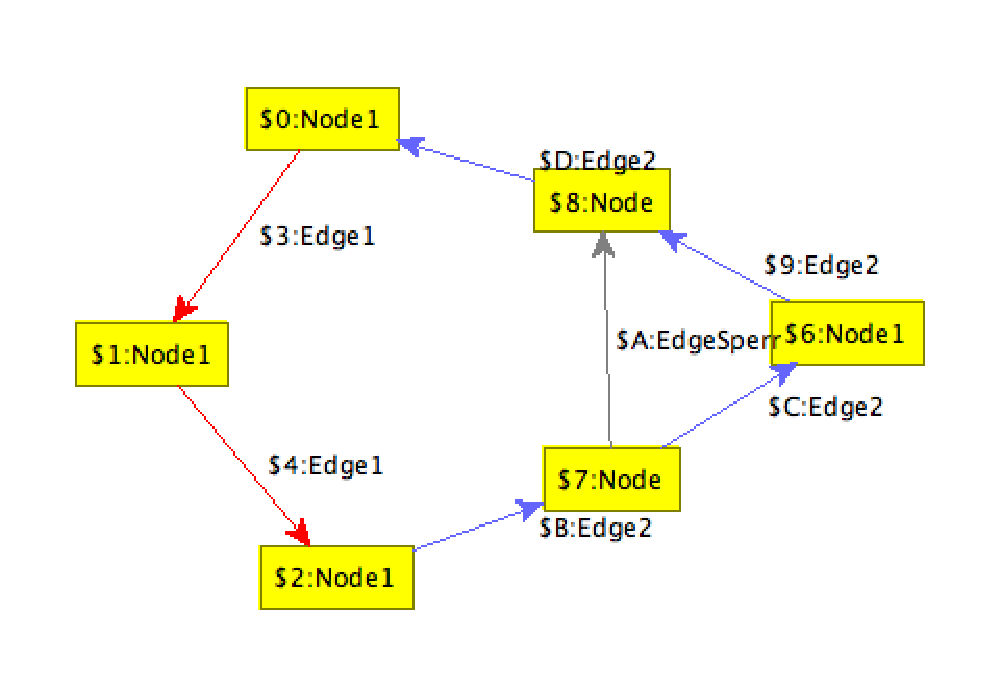
\includegraphics[width=\linewidth]{fig/debug3tra}}
\end{center}
The following table shows the ``break points'' of further debug commands, entered one after another:
\begin{center}
  \begin{tabular}{|l|l|} \hline
    \textbf{Command} & \textbf{Active rule} \\ \hline
    \texttt{s} & \texttt{makeFlake1} \\
    \texttt{o} & \texttt{beautify} \\
    \texttt{s} & \texttt{doNothing} \\
    \texttt{s} & \texttt{beautify} \\ 
    \texttt{u} & \texttt{beautify} \\ 
    \texttt{o} & \texttt{makeFlake2} \\
    \texttt{r} & --- \\ \hline
  \end{tabular}
\end{center}
\end{example}   
\end{figure}


\section{Backend Commands}
\label{backend}

\GrG\ is built to support multiple backends implementing the model and action interfaces of libGr.
This is roughly comparable to the different storage engines MySQL offers.
Currently only one backend is available, the libGr search plan backend, or short LGSPBackend.

\subsection{Backend selection and custom commands}

\begin{rail}
  'select' 'backend' Filename ( ( ) | ':' Parameters )
\end{rail}\ixkeyw{select}\ixkeyw{backend}
Selects a \indexed{backend} that handles graph and rule representation.
\emph{Filename} has to be a .NET assembly (e.g.\ \texttt{lgspBackend.dll}\indexmain{LGSPBackend}).
Comma-separated \indexed{parameter}s can be supplied optionally; if so, the backend must support these parameters.
By default the LGSPBackend is used.

\begin{rail}
  'show' 'backend'
\end{rail}\nopagebreak\ixkeyw{show}\ixkeyw{backend}
List all the parameters supported by the currently selected backend.
The parameters can be provided to the \texttt{select backend} command.

\begin{rail}
  'custom' 'graph' ( ( ) | SpacedParameters )
\end{rail}\ixkeyw{custom}\ixkeyw{graph}
Executes a command specific to the current backend.
If \emph{SpacedParameters} is omitted, a list of available commands will be displayed (for the LGSP backend see Sections~\ref{custom}).


\subsection{LGSPBackend Custom Commands}
\label{custom}

The \indexed{LGSPBackend} supports the following custom commands:

\begin{rail}
  'custom' 'graph' ('analyzegraph' | 'analyze') 
\end{rail}\ixkeyw{custom}\ixkeyw{graph}\ixkeyw{analyze}\ixkeyw{analyzegraph}
Analyzes\indexmain{analyzing graph} the current working graph.
The analysis data provides vital information for efficient \indexed{search plan}s.
Analysis data is available as long as \GrShell\ is running, i.e.\ when the working graph changes, the analysis data is still available but maybe obsolete.

\begin{rail}
  'custom' 'graph' 'setmaxmatches' Number
\end{rail}\ixkeyw{custom}\ixkeyw{graph}\ixkeyw{setmaxmatches}
Sets the maximum amount of possible pattern matches to \emph{Number}.
This command affects the expression \texttt{[\emph{Rule}]}.
If \emph{Number} is less or equal to zero, the constraint is reset.

\begin{rail}
  'custom' 'graph' 'optimizereuse' BoolLit
\end{rail}\ixkeyw{custom}\ixkeyw{graph}\ixkeyw{optimizereuse}
If set to false it prevents deleted elements from getting reused in a rewrite (i.e. it disables a performance optimization).
If set to true, new elements may not be discriminable anymore from already deleted elements using object equality, hash maps, etc.
					
\begin{rail}
  'custom' 'actions' 'gensearchplan' (Action+)
\end{rail}\ixkeyw{custom}\ixkeyw{actions}\ixkeyw{gensearchplan}
Creates a search plan (and executable code from it) for each rewrite rule \emph{Action} using the data from analyzing the graph (\texttt{custom graph analyze}).
Otherwise a \indexed{default search plan} is used. 
Analyzing and search plan/code generation themselves take some time, but they can lead to massively faster pattern matching, thus overall execution times
(the less uniform the type distribution and edge wiring between the nodes is, the higher are the improvements to be expected).
During the analysis phase the host graph must be in a shape ``similar'' to its shape when the main amount of work is done
(there may be some trial-and-error steps at different time points needed to get the overall most efficient search plan.)
A search plan is available as long as the current rule set remains loaded. 
Specify multiple rewrite rules instead of using multiple commands for each rule to improve the search plan generation performance.

\begin{rail}
  'custom' 'actions' 'dumpsourcecode' BoolLit
\end{rail}\ixkeyw{custom}\ixkeyw{actions}\ixkeyw{dumpsourcecode}
If set to true, C\# files will be dumped for the newly generated searchplans (similar to the \texttt{-keep} option of the generator).



\chapter{Examples}
\label{anexample}

%%%%%%%%%%%%%%%%%%%%%%%%%%%%%%%%%%%%%%%%%%%%%%%%%%%%%%%%%%%%%%%%%%%%%%%%%%%%%%%%%%%%%%%%%%%%%%%%
\section{Fractals}\indexmain{example}
\label{fractals}
The \GrG\ package ships with samples for fractal generation. We will construct the \indexed{Sierpinski triangle} and the \indexed{Koch snowflake}. They are created by consecutive rule applications starting with the initial host graphs
\begin{center}
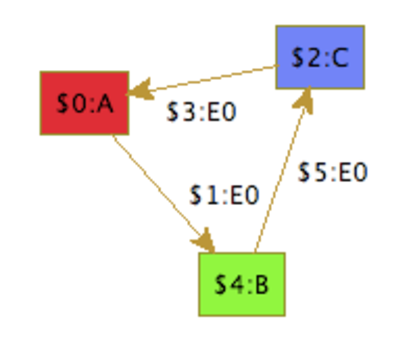
\includegraphics[width=4cm]{fig/startsir}\quad\quad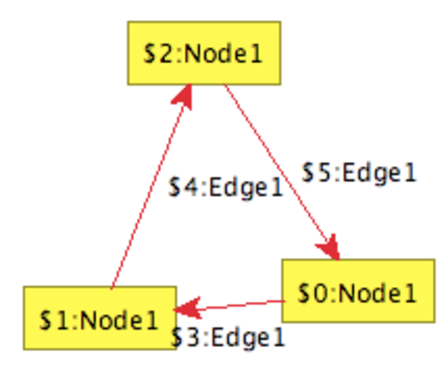
\includegraphics[width=4cm]{fig/startkoch}
\end{center}
for the Sierpinski triangle resp.\ the Koch snowflake. 
First of all we have to compile the model and rule set files. So execute in \GrG's \texttt{bin} directory
\begin{verbatim}
GrGen.exe ..\specs\sierpinski.grg
GrGen.exe ..\specs\snowflake.grg
\end{verbatim}
or
\begin{verbatim}
mono GrGen.exe ../specs/sierpinski.grg
mono GrGen.exe ../specs/snowflake.grg
\end{verbatim}
respectively. If you are on a Unix-like system you have to adjust the path separators of the \GrShell\ scripts. Just edit the first three lines of \texttt{/test/Sierpinski.grs} and \texttt{/test/Snowflake.grs}. And as we have the file \texttt{Sierpinski.grs} already opened, we can increase the number of iterations to get even more beautiful graphs\footnote{Be careful: The running time increases exponentially in the number of iterations.}. Just follow the comments. Be careful when increasing the number of iterations of Koch's snowflake---\yComp's \indexed{layout algorithm} might need some time and attempts to layout it nicely.
We execute the Sierpinski script by
\begin{verbatim}
GrShell.exe ..\test\Sierpinski.grs
\end{verbatim}
or
\begin{verbatim}
mono GrShell.exe ../test/Sierpinski.grs
\end{verbatim}
respectively. Because both of the scripts are using the debug mode, we complete execution by typing \texttt{r}(un). See Section~\ref{grsthings} for further information. The resulting graphs should look like Figures~\ref{figsierp} and~\ref{figsnowflake}.
\begin{figure}[htbp]
  \centering
  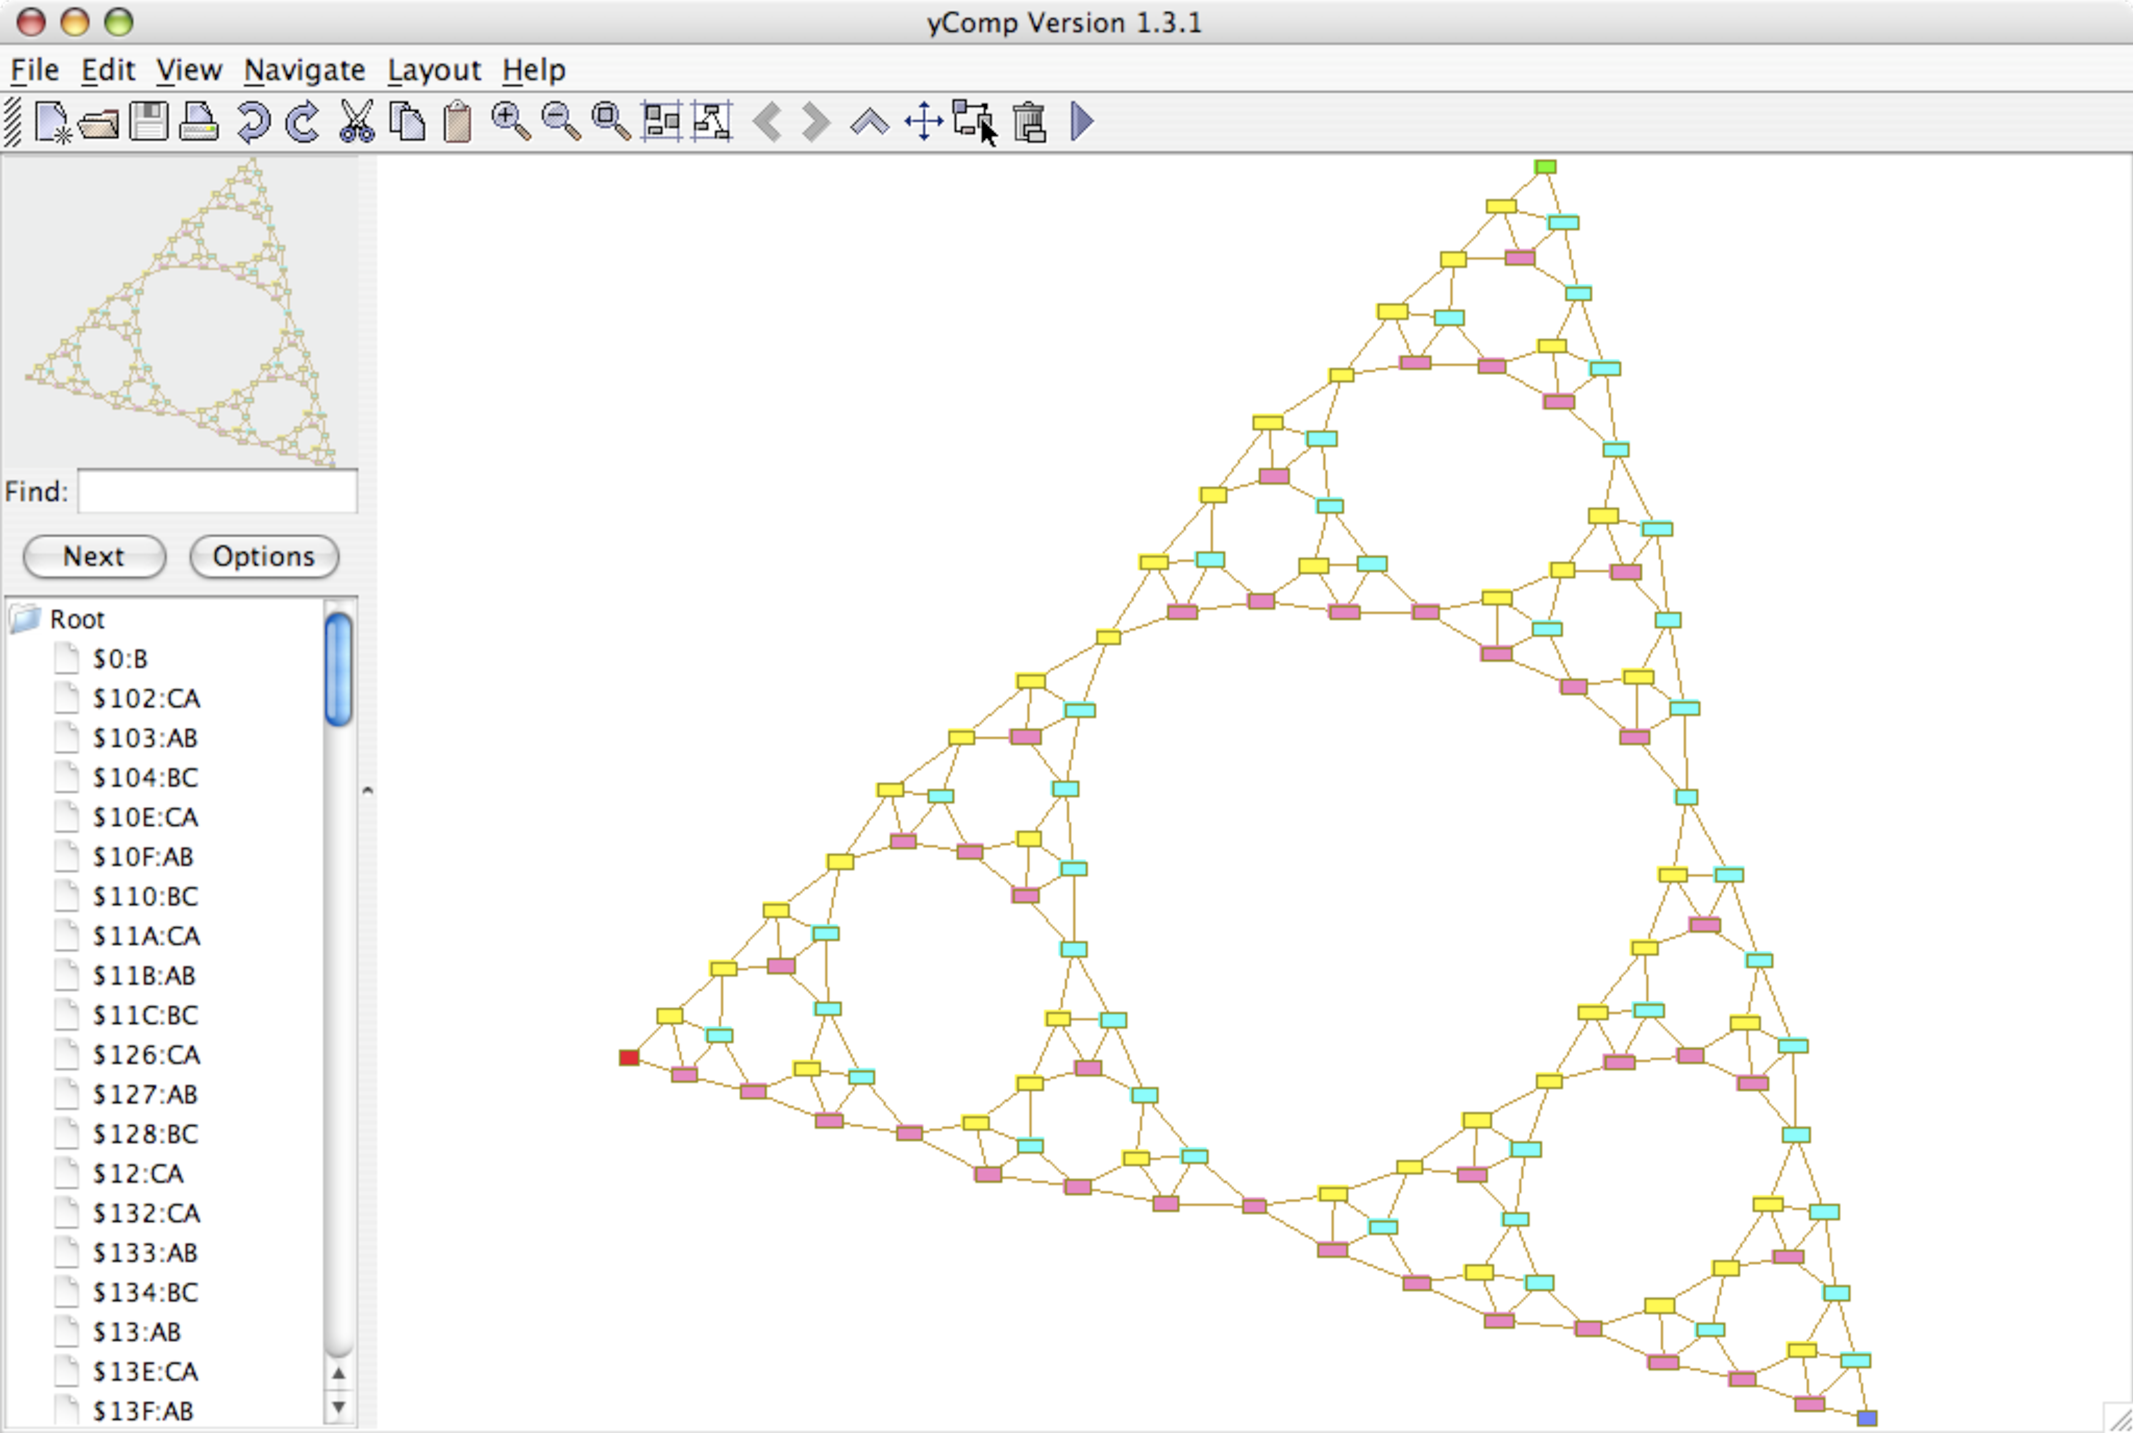
\includegraphics[width=\textwidth]{fig/sierpinski}
  \caption{Sierpinski triangle}
  \label{figsierp}
\end{figure}
\begin{figure}[htbp]
  \centering
  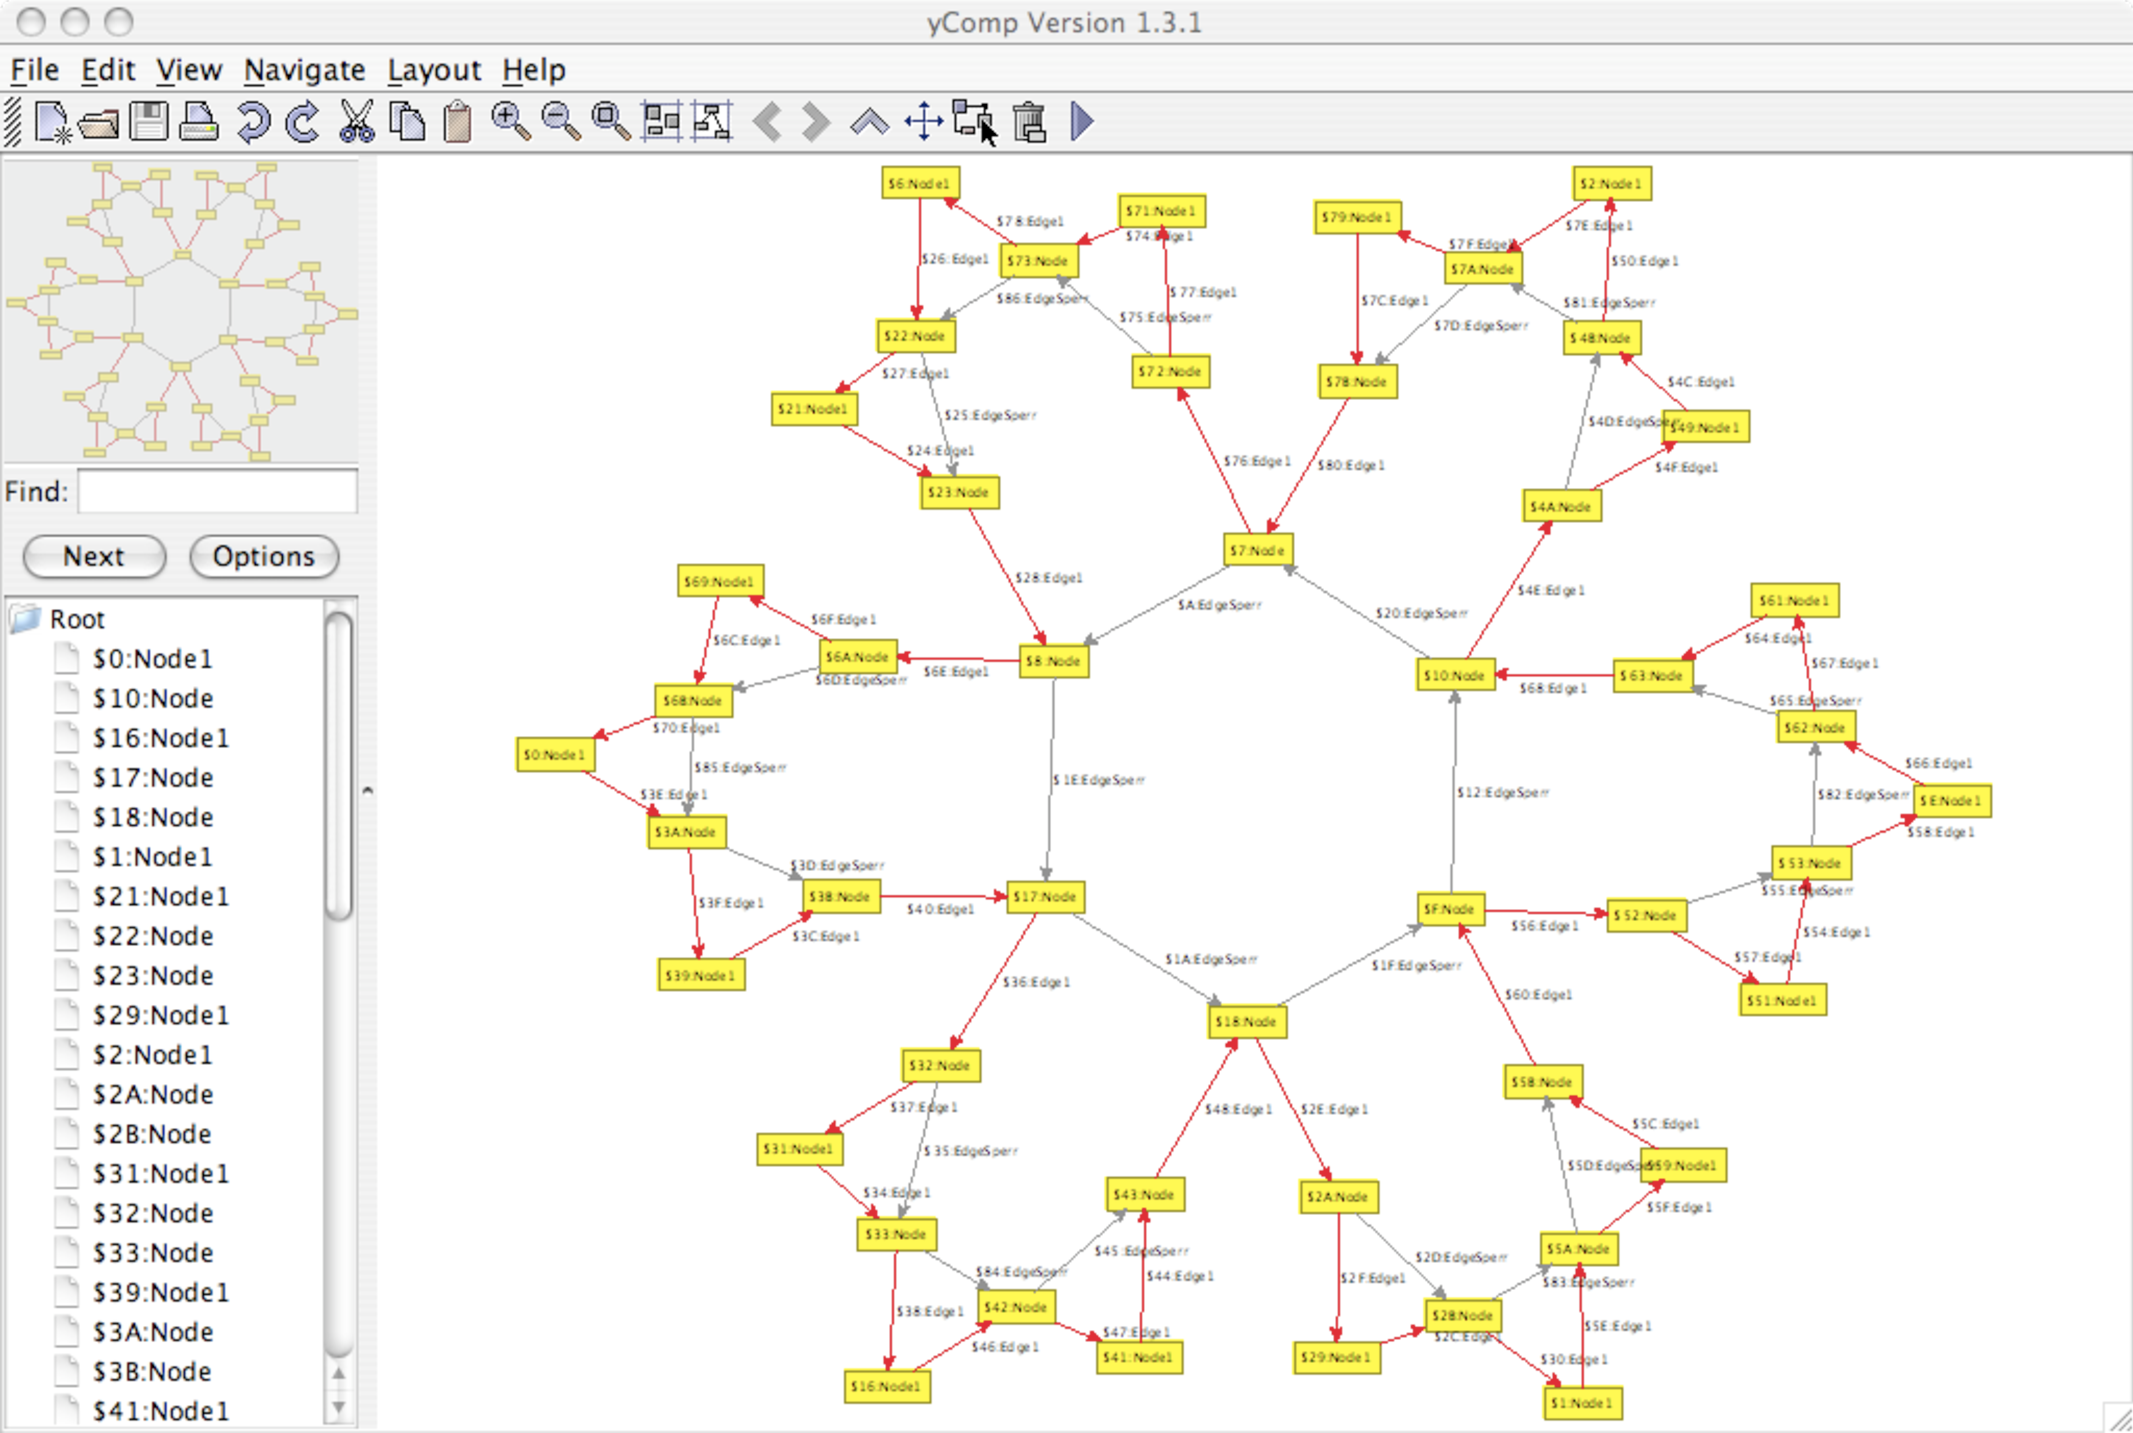
\includegraphics[width=\textwidth]{fig/snowflake}
  \caption{Koch snowflake}
  \label{figsnowflake}
\end{figure}
\vfill\pagebreak


%%%%%%%%%%%%%%%%%%%%%%%%%%%%%%%%%%%%%%%%%%%%%%%%%%%%%%%%%%%%%%%%%%%%%%%%%%%%%%%%%%%%%%%%%%%%%%%%
\section{Busy Beaver}\indexmain{example}
We want \GrG\ to work as hard as a \indexed{busy beaver}~\cite{Kro:07,Dew:84}. Our busy beaver is a Turing machine that has got five states plus a ``halt''-state; it writes 1,471 bars onto the tape and terminates~\cite{MB:00}. So first of all we design a Turing machine as graph model. Besides, this example shows that \GrG\ is \indexed{Turing complete}.

We use the graph model and the rewrite rules to define a general Turing machine. Our approach is to basically draw the machine as a graph. The busy beaver logic is implemented by rule applications in \GrShell.

%-----------------------------------------------------------------------------------------------
\subsection{Graph Model}
The tape will be a chain of \texttt{TapePosition} nodes connected by right edges. A cell value is modeled by a reflexive \texttt{value} edge, attached to a \texttt{TapePosition} node. The leftmost and the rightmost cells (\texttt{TapePosition}) do not have an incoming and outgoing edge respectively. Therefore we have the node constraint $[0:1]$.
\begin{grgen}[firstnumber=last]
node class TapePosition; 
edge class right
  connect TapePosition[0:1] --> TapePosition[0:1];
  
edge class value
  connect TapePosition[1] --> TapePosition[1];  
edge class zero  extends value;
edge class one   extends value;
edge class empty extends value;

\end{grgen}
Furthermore we need states and transitions. 
The machine's current configuration is modeled with a \texttt{RWHead} edge pointing to a \texttt{TapePosition} node. 
\texttt{State} nodes are connected with \texttt{WriteValue} nodes via \texttt{value} edges, a \texttt{moveLeft}/\texttt{moveRight}/\texttt{dontMove} edge leads from a \texttt{WriteValue} node to the next state (cf.~the picture on page \pageref{fig:bbstart}).
\begin{grgen}[firstnumber=last]
node class State;

edge class RWHead;

node class WriteValue;
node class WriteZero extends WriteValue;
node class WriteOne extends WriteValue;
node class WriteEmpty extends WriteValue; 

edge class moveLeft;
edge class moveRight;
edge class dontMove;
\end{grgen}

%-----------------------------------------------------------------------------------------------
\subsection{Rule Set}
Now the rule set: We begin the rule set file \texttt{Turing.grg} with
\begin{grgen}[firstnumber=1] 
using TuringModel;

\end{grgen}
We need rewrite rules for the following steps of the Turing machine:
\begin{enumerate}
  \item Read the value of the current tape cell and select an outgoing edge of the current state.
  \item Write a new value into the current cell, according to the sub type of the \texttt{WriteValue} node.
  \item Move the read-write-head along the tape and select a new state as current state. 
\end{enumerate}
As you can see a transition of the Turing machine is split into two graph rewrite steps: Writing the new value onto the tape and performing the state transition. We need eleven rules: Three rules for each step (for ``zero'', ``one'', and ``empty'') and two rules for extending the tape to the left and the right, respectively.
\begin{grgen}[firstnumber=last] 
rule readZeroRule {
	s:State -h:RWHead-> tp:TapePosition -:zero-> tp;
	s -:zero-> wv:WriteValue;
	modify {
		delete(h);
		wv -:RWHead-> tp;
	}
}      

\end{grgen}
We take the current state \texttt{s} and the current cell \texttt{tp} which is implicitly given by the unique \texttt{RWHead} edge and check whether the cell value is zero. Furthermore we check if the state has a transition for zero. The replacement part deletes the \texttt{RWHead} edge between \texttt{s} and \texttt{tp} and adds it between \texttt{wv} and \texttt{tp}. The remaining rules are analogous:
\begin{grgen}[firstnumber=last] 
rule readOneRule {
	s:State -h:RWHead-> tp:TapePosition -:one-> tp;
	s -:one-> wv:WriteValue;
	modify {
		delete(h);
		wv -:RWHead-> tp;
	}
}

rule readEmptyRule {
	s:State -h:RWHead-> tp:TapePosition -:empty-> tp;
	s -:empty-> wv:WriteValue;
	modify {
		delete(h);
		wv -:RWHead-> tp;
	}
}

rule writeZeroRule {
	wv:WriteZero -rw:RWHead-> tp:TapePosition -:value-> tp;
	replace {
		wv -rw-> tp -:zero-> tp;
	}	
}

rule writeOneRule {
	wv:WriteOne -rw:RWHead-> tp:TapePosition -:value-> tp;
	replace {
		wv -rw-> tp -:one-> tp;
	}	
}

rule writeEmptyRule {
	wv:WriteEmpty -rw:RWHead-> tp:TapePosition -:value-> tp;
	replace {
		wv -rw-> tp -:empty-> tp;
	}	
}

rule moveLeftRule {
	wv:WriteValue -:moveLeft-> s:State;
	wv -h:RWHead-> tp:TapePosition <-r:right- ltp:TapePosition;
	modify {
		delete(h);
		s -:RWHead-> ltp;
	}
}

rule moveRightRule {
	wv:WriteValue -:moveRight-> s:State;
	wv -h:RWHead-> tp:TapePosition -r:right-> rtp:TapePosition;
	modify {
		delete(h);
		s -:RWHead-> rtp;
	}
}

rule dontMoveRule {
	wv:WriteValue -:dontMove-> s:State;
	wv -h:RWHead-> tp:TapePosition;
	modify {
		delete(h);
		s -:RWHead-> tp;
	}
}

rule ensureMoveLeftValidRule {
	wv:WriteValue -:moveLeft-> :State;
	wv -:RWHead-> tp:TapePosition;
	negative {
		tp <-:right-;
	}
	modify {
		tp <-:right- ltp:TapePosition -:empty-> ltp;
	}
}

rule ensureMoveRightValidRule {
	wv:WriteValue -:moveRight-> :State;
	wv -:RWHead-> tp:TapePosition;
	negative {
		tp -:right->;
	}
	modify {
		tp -:right-> rtp:TapePosition -:empty-> rtp;
	}
}
\end{grgen}
Have a look at the negative conditions within the \texttt{ensureMove\dots} rules. They ensure that the current cell is indeed at the end of the tape: An edge to a right/left neighboring cell must not exist. Now don't forget to compile your model and the rule set with \texttt{GrGen.exe} (see Section~\ref{fractals}).

%-----------------------------------------------------------------------------------------------
\subsection{Rule Execution with \GrShell}

Finally we construct the busy beaver and let it work with \GrShell. The following script starts with building the Turing machine that is modeling the six states with their transitions in our Turing machine model:
\begin{grshell}[firstnumber=1] 
select backend "../bin/lgspBackend.dll"
new graph "../lib/lgsp-TuringModel.dll" "Busy Beaver"
select actions "../lib/lgsp-TuringActions.dll"

# Initialize tape
new tp:TapePosition($="Startposition")
new tp -:empty-> tp

# States
new sA:State($="A")
new sB:State($="B")
new sC:State($="C")
new sD:State($="D")
new sE:State($="E")
new sH:State($ = "Halt")

new sA -:RWHead-> tp

# Transitions: three lines per state and input symbol for
#   - updating cell value
#   - moving read-write-head
# respectively

new sA_0: WriteOne
new sA -:empty-> sA_0
new sA_0 -:moveLeft-> sB

new sA_1: WriteOne
new sA -:one-> sA_1
new sA_1 -:moveLeft-> sD

new sB_0: WriteOne
new sB -:empty-> sB_0
new sB_0 -:moveRight-> sC

new sB_1: WriteEmpty
new sB -:one-> sB_1
new sB_1 -:moveRight-> sE

new sC_0: WriteEmpty
new sC -:empty-> sC_0
new sC_0 -:moveLeft-> sA

new sC_1: WriteEmpty
new sC -:one-> sC_1
new sC_1 -:moveRight-> sB

new sD_0: WriteOne
new sD -:empty-> sD_0
new sD_0 -:moveLeft->sE

new sD_1: WriteOne
new sD -:one-> sD_1
new sD_1 -:moveLeft-> sH

new sE_0: WriteOne
new sE -:empty-> sE_0
new sE_0 -:moveRight-> sC

new sE_1: WriteOne
new sE -:one-> sE_1
new sE_1 -:moveLeft-> sC

\end{grshell}
\quad\\Our busy beaver looks like this:\label{fig:bbstart}
\begin{center}
  \fbox{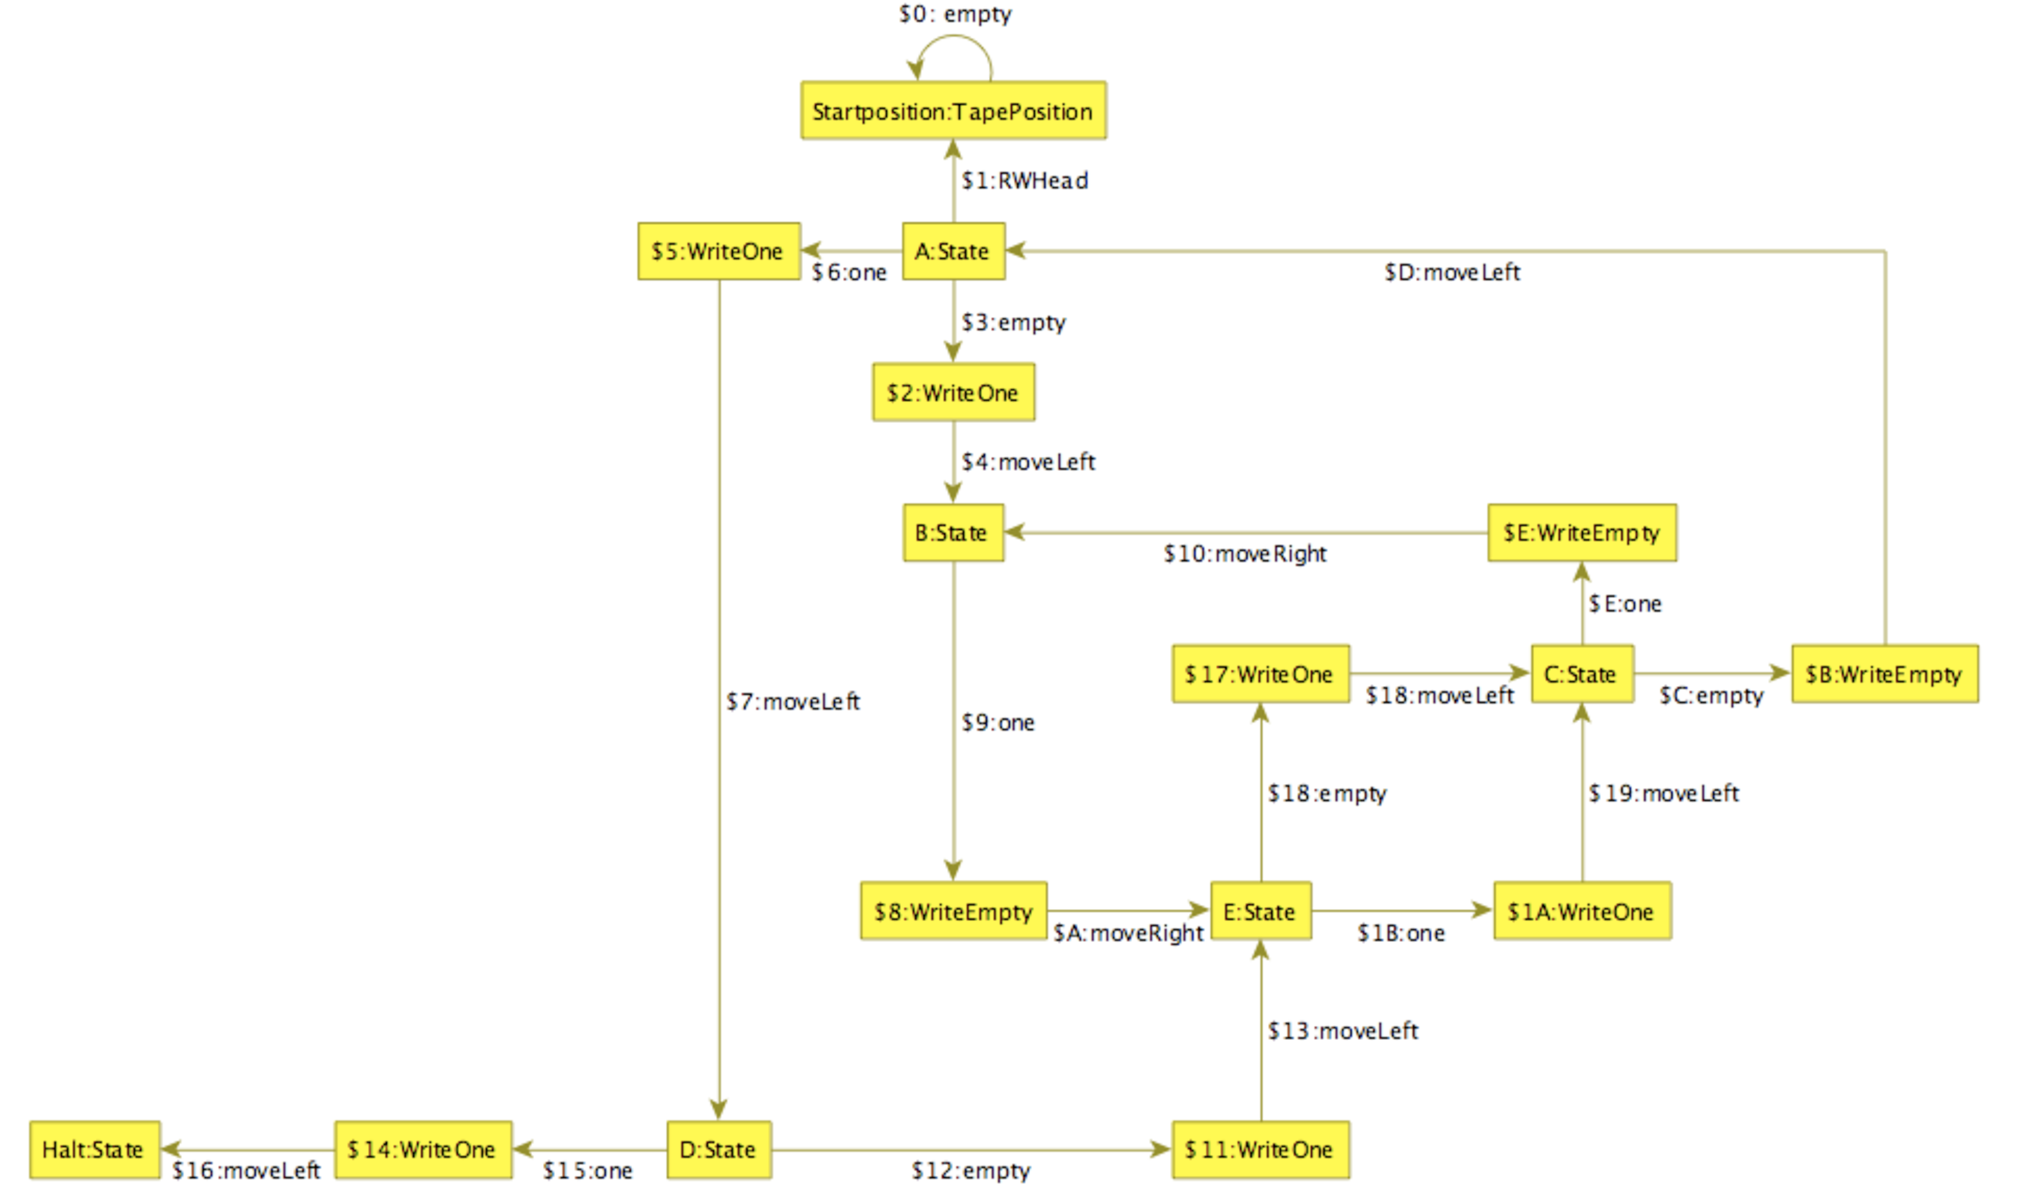
\includegraphics[width=\linewidth-2\fboxsep-2\fboxrule]{fig/bbstart}}
\end{center}

We have an initial host graph now. The graph rewrite sequence is quite straight forward and generic to the Turing graph model. Note that for each state the ``\texttt{\dots Empty\dots} | \texttt{\dots One\dots}'' selection is unambiguous.
%\pagebreak %HACK
\begin{grshell}[firstnumber=last]
  xgrs ((readOneRule | readEmptyRule) & (writeOneRule | writeEmptyRule) & (ensureMoveLeftValidRule | ensureMoveRightValidRule) & (moveLeftRule | moveRightRule))[32]

\end{grshell}
\quad\\We interrupt the machine after 32 iterations and look at the result so far:
\begin{center}
  \fbox{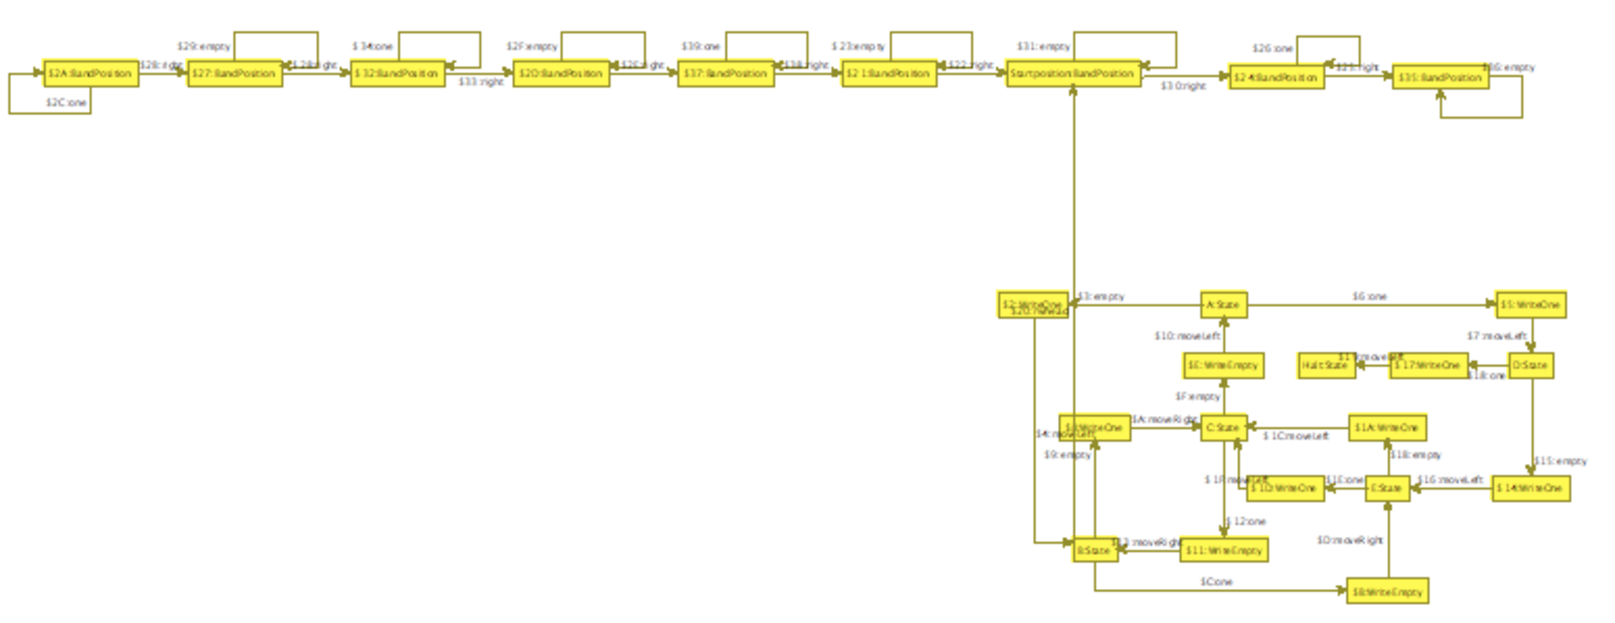
\includegraphics[width=\linewidth-2\fboxsep-2\fboxrule]{fig/bbmiddle}}
\end{center}
In order to improve the performance we generate better \indexed{search plan}s. This is a crucial step for execution time: With the initial search plans the beaver runs for 1 minute and 30 seconds. With improved search plans after the first 32 steps he takes about 8.5 seconds\footnote{On a Pentium 4, 3.2Ghz, with 2GiB RAM.}.
\begin{grshell}[firstnumber=last]
custom graph analyze_graph
custom actions gen_searchplan readOneRule readEmptyRule writeOneRule writeEmptyRule ensureMoveLeftValidRule ensureMoveRightValidRule moveLeftRule moveRightRule

\end{grshell}

Let the beaver run:
\begin{grshell}[firstnumber=last]
  xgrs ((readOneRule | readEmptyRule) & (writeOneRule | writeEmptyRule) & (ensureMoveLeftValidRule | ensureMoveRightValidRule) & (moveLeftRule | moveRightRule))*
\end{grshell}




\thebibliography{99}
\bibitem{geiss} R. Geiß et al.: \emph{\GrG: A Fast SPO-Based Graph Rewriting Tool} in Graph Transformations, number 4178 in LNCS, pages 383-397, Springer, 2006
\bibitem{kroll} M. Kroll: \emph{Portierung des C-Anteils des Graphersetzungssystems \GrG\ nach C\# mit Erweiterungen}, Studienarbeit, Fakultät für Informatik, Universität Karlsruhe, 2007
\bibitem{hack} S. Hack: \emph{Graphersetzung für Optimierung in der Codeerzeugung} Diplomarbeit, Fakultät für Informatik, Universität Karlsruhe, 2003
\bibitem{grund} D. Grund: \emph{Negative Anwendungsbedingungen für den Graphersetzer \GrG} Studienarbeit, Fakultät für Informatik, Universität Karlsruhe, 2004 
\bibitem{adam} A. Szalkowski: \emph{Negative Anwendungsbedingungen für das suchprogrammbasierte Backend von GrGen} Studienarbeit, Fakultät für Informatik, Universität Karlsruhe, 2005
\bibitem{batz} G. Batz: \emph{Graphersetzung für eine Zwischendarstellung im Übersetzerbau} Diplomarbeit, Fakultät für Informatik, Universität Karlsruhe, 2005
\bibitem{pascal} K. Jensen, N. Wirth: \emph{Pascal User Manual and Report} Springer, $^41991$
\bibitem{bb} A. Dewdney: \emph{A computer trap for the Busy Beaver, the hardest-working machine} Scientific American, 251(2), pages 10-12, 16, 17, August 1984
\bibitem{beaver} H. Marxen, J. Buntrock: \emph{Old list of record TMs.}\\ http://www.drb.insel.de/~heiner/BB/index.html. Version: August 2000

\end{document}
